% Plain-language review document (explaneat plain-language review), v5.
\documentclass[a4paper,10pt]{article}
\usepackage[margin=1.8cm]{geometry}
\usepackage{amsmath}
\usepackage{amssymb}
\usepackage{booktabs}
\usepackage{tabularx}
\usepackage{graphicx}
\usepackage[table,usenames,dvipsnames]{xcolor}
\usepackage{tikz}
\usetikzlibrary{arrows.meta,fit,backgrounds,positioning,calc}
\usetikzlibrary{shapes.geometric}
\usepackage{longtable}
\usepackage{pdflscape}
\usepackage{float}
\usepackage[font=small,labelfont=bf]{caption}
\usepackage{array}
\usepackage[unicode=true,hidelinks]{hyperref}
\setcounter{tocdepth}{3}
\setcounter{secnumdepth}{3}
% Review markers, copied from dissertation.tex (7 Nov 2026) for standalone builds.
\newif\ifreviewmarks
\reviewmarkstrue
\newcommand{\reviewrule}{\noindent{\color{BrickRed}\rule{\linewidth}{0.8pt}}}
\newenvironment{drafted}[1][]{%
  \ifreviewmarks\par\addvspace{\medskipamount}\reviewrule\par\nopagebreak
  \noindent{\color{BrickRed}\sffamily\footnotesize\textbf{Thesis Draft}\quad #1\hfill review}\par\nopagebreak\smallskip\fi}{%
  \ifreviewmarks\par\smallskip\noindent{\color{BrickRed}\sffamily\footnotesize end of thesis draft}\par\nopagebreak\reviewrule\par\medskip\fi}
\newcommand{\figreview}[1]{\ifreviewmarks\par\smallskip{\color{NavyBlue}\sffamily\footnotesize\textbf{Figure note:} #1}\par\fi}
\begin{document}
\begin{center}{\Large\bfseries Plain-language explanation: churn100-s7-c1\par}\vspace{2mm}{\small AI-assisted drafts for review. Nothing here has been verified by a person.\par}\end{center}
\noindent\textbf{How to read this.} Explanations are built up but read down: the summary first, then each part from the whole model down, in plain words, each sentence followed by the claims it rests on (C01, C02, \ldots; every cited claim was computed on the model and checked). Numbers are changes in predicted risk for a typical patient. The technical record (original hypotheses, formulas, evidence tables with the test check, ranges and n) is at the end. The text describes what the model does, not the world; whether it is plausible is for the reviewer to judge.
\par\medskip\noindent\textbf{What changed in v5e (figures).} v5e: every diagram is a numbered figure with a caption (list of figures after the contents) and the text refers to it; the whole-network figure has its own landscape page, scaled to the page, with a short caption and its description in the text; an input used by several parts is drawn under each of them (same input, repeated for readability, dotted outline); and an appendix figure shows the trained network before any explanation (no parts, no splits).
\par\medskip\noindent\textbf{What changed in v5c (tables and diagrams).} v5c: the evidence tables are landscape, compact and shaded by row, with the header repeated on every page (longtable and pdflscape, used in this review PDF only; the thesis preamble has neither). In the diagrams each input is drawn once, in a shared row along the bottom (the explanation's split copies of an input are listed in the technical detail instead), every cluster has one output rectangle with its plain name, the inputs that feed the output directly meet in a drawn 'sum', and a one-line legend explains the edges.
\par\medskip\noindent\textbf{What changed in v5b (diagrams).} v5b uses one grouping everywhere, the annotation hierarchy: the summary's diagram is the same picture as the whole model's section, and a part that is itself a weighted sum (blood pressure with cholesterol) is a part of its own, described as one that adds up, so the text counts three parts throughout; the lint checks every 'N parts' against the hierarchy. A full-structure diagram follows the summary: every node and connection, nested by part, with the inputs that feed the output directly in their own cluster and the unused input columns listed. Each section from the top down adds its own region of that diagram, with stubs for connections from or to other parts; each connection is drawn in exactly one section. The gate's text now says that it lowers the risk for the patients it acts on, and that more vessels and higher cholesterol take that lowering away; its vessel statements are one per group.
\par\medskip\noindent\textbf{What changed in v5 (read down).} v5 reads the explanation down. The summary (one line, a diagram, one paragraph per block) is as in v4, except that the paragraph on what adds up is split into protective items, risk-raising items and rare results, and an input that also feeds a part is quoted with its direct contribution only (the rest is in that part's paragraph). Then the document walks the annotation hierarchy from the whole model down: for each part a plain hypothesis (what it does for the prediction), plain evidence (what was checked and what it showed; for a part made of others, what they are and how they combine), a diagram one level down and where to read on. The original hypotheses, closed forms and evidence tables are in 'Technical detail' at the end. Statements about structure (what a part is made of, a copy of another part, a formula that reproduces it) are now claims of their own, checked on the graph and the data.
\par\medskip\noindent\textbf{v4.} v4 follows the structure of the explanation. The summary opens with one line and a diagram at the same grouping, then gives one paragraph per top-level block of the annotation hierarchy: one for everything that adds up independently (the inputs that feed the model score directly, and parts that are a weighted sum), and one for each part that combines its inputs in another way: what it combines, how, and for whom. 'Parts in detail' follows the hierarchy below that, with a diagram one level down for each part that contains others. The prose no longer says 'clearly', 'slightly', 'consistently' or 'on the training data only': the numbers carry it, and the test check, the ranges and n stay in the evidence tables. Only genuinely small groups are marked, with their n. The lint rejects the confidence words and checks the block structure.
\tableofcontents
\listoffigures
\clearpage
\begin{drafted}[plain-language layer: churn100-s7-c1]
\section{churn100-s7-c1}
\noindent{\small Genome \texttt{32d24e98-266e-450c-88c8-5bdc1abbf5dd}, explanation \texttt{b370983e-3d7d-40c8-8b8f-f37c41a96cc1}. Split: train primary (n=4000), test as a check (n=1000). Claims: 119, verified 109, not supported 10.\par}
\noindent{\small\textcolor{BrickRed}{AI-assisted draft for review (unverified)}\par}\smallskip
\noindent{\footnotesize Reference (typical) customer: the typical customer: the median training customer for every number and the most common training category for every category (not a real customer). account length: 100; area code: area code 415; international plan: no international plan; number customer service calls: 1 calls; number vmail messages: 0 messages; state: West Virginia; total day calls: 100 calls; total day charge: 30.69 US dollars; total day minutes: 180 minutes; total eve calls: 100 calls; total eve charge: 17.12 US dollars; total eve minutes: 201 minutes; total intl calls: 4 calls; total intl charge: 2.78 US dollars; total intl minutes: 10 minutes; total night calls: 100 calls; total night charge: 9.02 US dollars; total night minutes: 200 minutes; voice mail plan: no voice-mail plan. Predicted chance that a customer leaves: 1\%.\par}
\subsection{Summary}
\noindent For a typical customer (in West Virginia, area code 415, no international or voice-mail plan, 1 call to customer service and median usage) the model predicts a chance of leaving of about 1\%; it adds up five parts: usage and service calls, the international plan, fixed-weight inputs, a voice-mail and South Dakota adjustment and state adjustments.\,{\scriptsize\textcolor{NavyBlue}{[C047]}} Figure~\ref{fig:churn100s7c1:summary} shows the model at this level: one box per paragraph below.
\par\medskip\noindent\fbox{\begin{minipage}{0.96\linewidth}\small\textbf{How to read the diagrams.} Edge colour is the sign of that one connection: blue positive, red negative; thicker is a larger weight. The outline and arrow on an input (and on a part's output box) is its overall effect on the final prediction, read from the verified claims: orange and up arrow raises it, teal and down arrow lowers it, grey and double arrow depends (it goes both ways, or differs between levels). A negative connection into a part that itself raises the prediction means that input lowers the prediction; through a hinge the overall effect can only be read from the claims, not from the edges. Up arrow means towards churn; down arrow, away from it. A double outline marks an input (or a part's output) that acts at a fixed rate everywhere: it adds the same amount to the score per unit, so it is explained by its rate alone (see 'Linear factors'); a dashed double outline, at a fixed rate on the observed data. The normal outline is an input whose effect switches on and off somewhere. For example, a voice-mail plan has a negative connection into 'Usage and service calls', a part that raises the predicted chance that a customer leaves, so a voice-mail plan lowers it.\end{minipage}}\par\medskip
\begin{figure}[H]\centering
\resizebox{!}{\ifdim\height>0.5\textheight 0.5\textheight\else\height\fi}{%
\resizebox{\ifdim\width>\linewidth\linewidth\else\width\fi}{!}{%
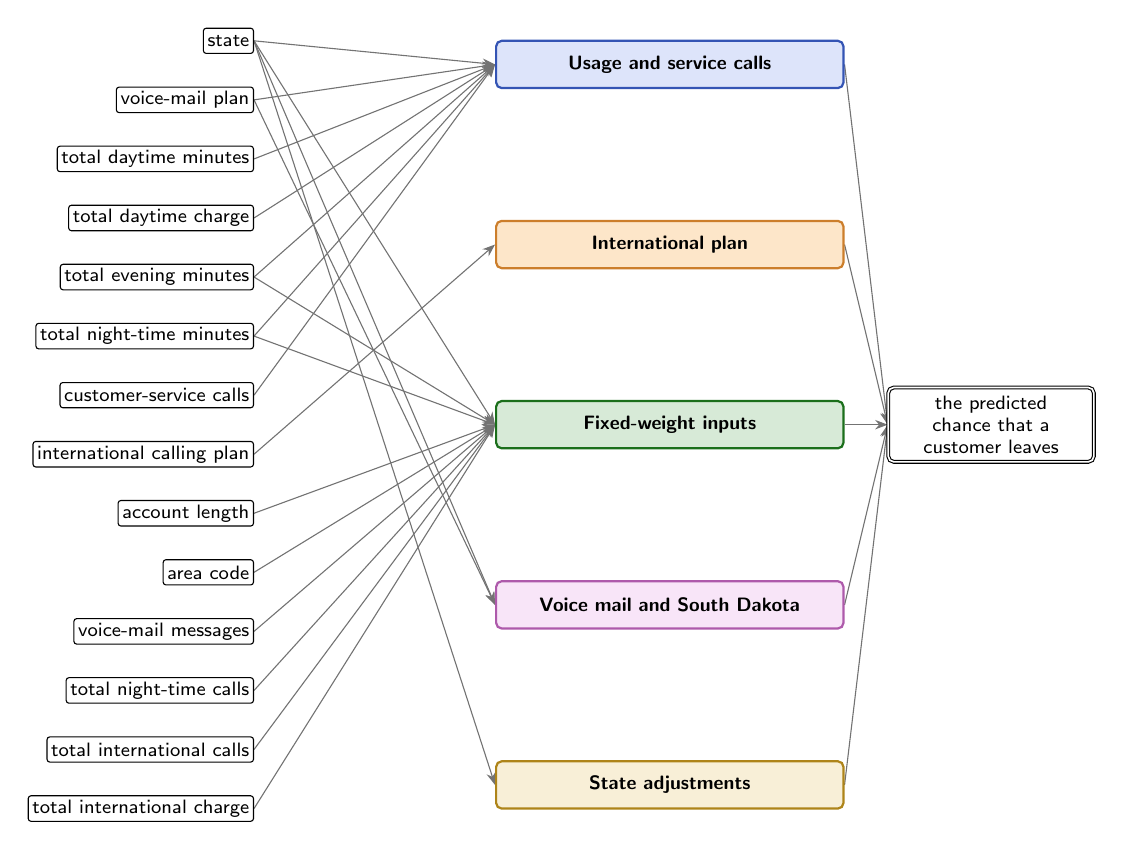
\begin{tikzpicture}[
  font=\sffamily\scriptsize, >={Stealth[length=1.6mm]},
  inp/.style={draw, rounded corners=1pt, fill=white, inner sep=1.5pt, minimum height=3.2mm, anchor=east},
  abox/.style={draw, thick, rounded corners=2pt, align=center, inner sep=3pt, minimum height=6mm, text width=42mm},
  outp/.style={draw, double, rounded corners=2pt, fill=white, align=center, inner sep=3pt, text width=24mm},
  agg/.style={draw=black!55},
]
\node[inp] (i0) at (0,4.875) {state};
\node[inp] (i1) at (0,4.125) {voice-mail plan};
\node[inp] (i2) at (0,3.375) {total daytime minutes};
\node[inp] (i3) at (0,2.625) {total daytime charge};
\node[inp] (i4) at (0,1.875) {total evening minutes};
\node[inp] (i5) at (0,1.125) {total night-time minutes};
\node[inp] (i6) at (0,0.375) {customer-service calls};
\node[inp] (i7) at (0,-0.375) {international calling plan};
\node[inp] (i8) at (0,-1.125) {account length};
\node[inp] (i9) at (0,-1.875) {area code};
\node[inp] (i10) at (0,-2.625) {voice-mail messages};
\node[inp] (i11) at (0,-3.375) {total night-time calls};
\node[inp] (i12) at (0,-4.125) {total international calls};
\node[inp] (i13) at (0,-4.875) {total international charge};
\node[abox, fill=RoyalBlue!18, draw=RoyalBlue!80!black] (b0) at (5.28,4.575) {\textbf{Usage and service calls}};
\node[abox, fill=BurntOrange!18, draw=BurntOrange!80!black] (b1) at (5.28,2.288) {\textbf{International plan}};
\node[abox, fill=ForestGreen!18, draw=ForestGreen!80!black] (b2) at (5.28,-0.0) {\textbf{Fixed-weight inputs}};
\node[abox, fill=Orchid!18, draw=Orchid!80!black] (b3) at (5.28,-2.288) {\textbf{Voice mail and South Dakota}};
\node[abox, fill=Goldenrod!18, draw=Goldenrod!80!black] (b4) at (5.28,-4.575) {\textbf{State adjustments}};
\node[outp] (out) at (9.36,0) {the predicted chance that a customer leaves};
\begin{scope}[on background layer]
\draw[->, agg, thin] (i0.east) -- (b0.west);
\draw[->, agg, thin] (i1.east) -- (b0.west);
\draw[->, agg, thin] (i2.east) -- (b0.west);
\draw[->, agg, thin] (i3.east) -- (b0.west);
\draw[->, agg, thin] (i4.east) -- (b0.west);
\draw[->, agg, thin] (i5.east) -- (b0.west);
\draw[->, agg, thin] (i6.east) -- (b0.west);
\draw[->, agg] (b0.east) -- (out.west);
\draw[->, agg, thin] (i7.east) -- (b1.west);
\draw[->, agg] (b1.east) -- (out.west);
\draw[->, agg, thin] (i0.east) -- (b2.west);
\draw[->, agg, thin] (i8.east) -- (b2.west);
\draw[->, agg, thin] (i9.east) -- (b2.west);
\draw[->, agg, thin] (i10.east) -- (b2.west);
\draw[->, agg, thin] (i4.east) -- (b2.west);
\draw[->, agg, thin] (i5.east) -- (b2.west);
\draw[->, agg, thin] (i11.east) -- (b2.west);
\draw[->, agg, thin] (i12.east) -- (b2.west);
\draw[->, agg, thin] (i13.east) -- (b2.west);
\draw[->, agg] (b2.east) -- (out.west);
\draw[->, agg, thin] (i0.east) -- (b3.west);
\draw[->, agg, thin] (i1.east) -- (b3.west);
\draw[->, agg] (b3.east) -- (out.west);
\draw[->, agg, thin] (i0.east) -- (b4.west);
\draw[->, agg] (b4.east) -- (out.west);
\end{scope}
\end{tikzpicture}}}%
\caption{The model at the level of the summary: one box per part.}
\label{fig:churn100s7c1:summary}
\end{figure}
\paragraph{Usage and service calls.} This part combines a usage score, built from daytime, evening and night-time minutes and the voice-mail plan, with calls to customer service, not as a simple sum.\,{\scriptsize\textcolor{NavyBlue}{[C060]}} Customer-service calls add only from about 3 calls upwards, for most customers slowly at first, then faster, but for some customers without a voice-mail plan they add nothing until a point, then steadily: going from 0 to 4 calls takes a typical customer from about 1\% to about 15\%.\,{\scriptsize\textcolor{NavyBlue}{[C055]}} Through it, daytime minutes add to the chance only above about 187 minutes for customers without a voice-mail plan, in an uneven way: for a typical customer, going from 0 to 271 minutes takes it from about 1\% to about 11\%.\,{\scriptsize\textcolor{NavyBlue}{[C056]}} Daytime minutes count more with more than 201 evening minutes, in an uneven way: from about 1\% to about 11\% between 112 and 249 minutes, against about 1\% to about 2\% with fewer.\,{\scriptsize\textcolor{NavyBlue}{[C067]}}
\paragraph{International plan.} This part reads the international plan alone and acts on the 380 of 4000 training customers who have one, 161 of whom left; for the typical customer it acts on, the chance is about 2\% without it and about 26\% with it.\,{\scriptsize\textcolor{NavyBlue}{[C078]}} For a typical customer, an international plan takes the chance of leaving from about 1\% to about 15\%.\,{\scriptsize\textcolor{NavyBlue}{[C077]}}
\paragraph{Fixed-weight inputs.} This part adds up many inputs with fixed weights, each moving a typical customer's chance by a few points at most: compared with most other states, Washington raises it to about 3\% and Montana to about 2\%, and Vermont, Rhode Island and Colorado lower it to under 1\%.\,{\scriptsize\textcolor{NavyBlue}{[C080, C081, C082, C084, C085]}} A higher international charge raises it steadily, from under 1\% at 1.84 to about 1\% at 3.70 US dollars, and more voice-mail messages and a longer account also raise it steadily, by less than a point.\,{\scriptsize\textcolor{NavyBlue}{[C083, C086, C098]}} More international calls lower it, each extra call taking away about the same, from about 1\% at 2 to under 1\% at 8 calls, and more evening and night-time minutes lower it steadily through this part, by less than a point.\,{\scriptsize\textcolor{NavyBlue}{[C087, C092, C096]}}
\paragraph{Voice mail and South Dakota.} This part reads the voice-mail plan and the state: through it, a customer in South Dakota has under 1\% instead of about 1\%, and a voice-mail plan also lowers a typical customer's chance to under 1\%.\,{\scriptsize\textcolor{NavyBlue}{[C108, C109]}}
\paragraph{State adjustments.} This part reads only the state: it moves a typical customer's chance from about 1\% in West Virginia to about 5\% in South Dakota and about 2\% in Indiana and in most other states, and keeps it under 1\% in Virginia (66 to 122 training customers per named state; the full list is in the technical detail).\,{\scriptsize\textcolor{NavyBlue}{[C111, C112, C114, C115]}}
\paragraph{The whole network.} Figure~\ref{fig:churn100s7c1:overview} (next page, landscape) draws every unit and connection of the explained model, nested by part: shaded clusters are the parts of the model and darker boxes the parts inside them; circles are hidden units (h1, h2, \ldots); each cluster's rectangle is its output, and a dashed `sum' stands for an addition the next unit does (drawn, not a unit of the model); the hexagon is the model's output. An input used by several parts is drawn under each of them (same label, dotted outline, the first copy marked with the number of copies): it is the same input, repeated for readability. Not used by the model (input columns with no connection): state: 28 of 51 levels, area code 408, area code 415, total daytime calls, total evening calls, total evening charge, total night-time charge, total international minutes.
\begin{landscape}
\begin{figure}[p]\centering
\resizebox{\linewidth}{!}{%
\definecolor{netup}{HTML}{D95F02}\definecolor{netdown}{HTML}{1B9E77}\definecolor{netmixed}{HTML}{7F7F7F}%
\begin{tikzpicture}[
  font=\sffamily\scriptsize, >={Stealth[length=1.4mm]},
  inp/.style={draw, circle, fill=white, minimum size=3.2mm, inner sep=0pt},
  hid/.style={draw, circle, fill=white, minimum size=5.2mm, inner sep=0.5pt, font=\sffamily\tiny},
  exitbox/.style={draw, thick, rectangle, fill=white, align=center, text width=17mm, minimum height=5mm, inner sep=1.5pt, font=\sffamily\tiny},
  sumbox/.style={draw, thick, dashed, rectangle, fill=white, align=center, text width=17mm, minimum height=5mm, inner sep=1.5pt, font=\sffamily\tiny},
  outp/.style={draw, thick, regular polygon, regular polygon sides=6, fill=white, minimum size=10mm, inner sep=0pt, font=\sffamily\tiny, align=center},
  stub/.style={draw, dashed, rounded corners=2pt, fill=white, align=center, inner sep=2pt, font=\sffamily\tiny, text width=15mm},
  inlab/.style={font=\sffamily\tiny, align=center, text width=15mm, inner sep=1pt, fill=white, fill opacity=0.8, text opacity=1},
  wpos/.style={draw=NavyBlue}, wneg/.style={draw=BrickRed}, wagg/.style={draw=black!45, line width=1.2pt},
  wmix/.style={draw=Plum},
]
\node[outp] (n0) at (23.655,10.2) {churn};
\node[hid] (n10552) at (7.165,7.3) {h10};
\node[hid] (n12726) at (38.91,1.9) {h11};
\node[hid] (n13164) at (40.41,1.9) {h12};
\node[hid] (n13420) at (41.91,1.9) {h13};
\node[hid] (n1406) at (4.26,1.9) {h3};
\node[hid] (n14351) at (6.415,5.95) {h14};
\node[hid] (n2067) at (43.41,1.9) {h4};
\node[hid] (n4344) at (7.915,5.95) {h5};
\node[hid] (n5667) at (44.91,1.9) {h6};
\node[exitbox] (n582) at (34.32,1.9) {Voice mail and South Dakota $\downarrow$};
\node[hid] (n5821) at (46.41,1.9) {h7};
\node[exitbox] (n6711) at (15.04,1.9) {International plan $\uparrow$};
\node[hid] (n7558) at (4.26,3.25) {h9};
\node[hid] (n879) at (4.26,4.6) {h2};
\node[exitbox] (nidentityxlin) at (24.23,1.9) {Fixed-weight inputs $\uparrow$};
\node[exitbox] (nidentityxusage) at (7.165,8.65) {Usage and service calls $\uparrow$};
\node[sumbox] (ncsumxxannx82) at (42.66,3.25) {sum: State adjustments $\updownarrow$};
\node[inp, densely dotted, thick, draw=netmixed, very thick] (ngrpxxstatexxannx82) at (42.66,0.0) {};
\path (ngrpxxstatexxannx82.south) node[inlab, anchor=north] (labngrpxxstatexxannx82) {state (23 of 51 used) ($\times$4) $\updownarrow$};
\node[inp, draw=netup, very thick] (ninxxtotalxdayxminutesxxannx83) at (4.5,0.0) {};
\path (ninxxtotalxdayxminutesxxannx83.south) node[inlab, anchor=north] (labninxxtotalxdayxminutesxxannx83) {total daytime minutes $\uparrow$};
\node[inp, draw=netup, very thick] (ninxxinternationalxplanxxannx81) at (15.04,0.0) {};
\path (ninxxinternationalxplanxxannx81.south) node[inlab, anchor=north] (labninxxinternationalxplanxxannx81) {an international plan $\uparrow$};
\node[inp, draw=netup, very thick] (ninxxtotalxdayxchargexxannx83) at (2.7,0.0) {};
\path (ninxxtotalxdayxchargexxannx83.south) node[inlab, anchor=north] (labninxxtotalxdayxchargexxannx83) {total daytime charge $\uparrow$};
\node[inp, draw=netup, very thick] (ninxxnumberxcustomerxservicexcallsxxannx83) at (9.9,0.0) {};
\path (ninxxnumberxcustomerxservicexcallsxxannx83.south) node[inlab, anchor=north] (labninxxnumberxcustomerxservicexcallsxxannx83) {customer-service calls $\uparrow$};
\node[inp, densely dotted, thick, draw=netmixed, very thick] (ngrpxxstatexxannx80) at (35.22,0.0) {};
\path (ngrpxxstatexxannx80.south) node[inlab, anchor=north] (labngrpxxstatexxannx80) {state (23 of 51 used) $\updownarrow$};
\node[inp, densely dotted, thick, draw=netmixed, very thick] (ngrpxxstatexxannx83) at (1.8,-1.05) {};
\path (ngrpxxstatexxannx83.south) node[inlab, anchor=north] (labngrpxxstatexxannx83) {state (23 of 51 used) $\updownarrow$};
\node[inp, densely dotted, thick, draw=netdown, very thick] (ninxxvoicexmailxplanxxannx80) at (33.42,0.0) {};
\path (ninxxvoicexmailxplanxxannx80.south) node[inlab, anchor=north] (labninxxvoicexmailxplanxxannx80) {a voice-mail plan ($\times$2) $\downarrow$};
\node[inp, densely dotted, thick, draw=netdown, very thick] (ninxxvoicexmailxplanxxannx83) at (0.9,0.0) {};
\path (ninxxvoicexmailxplanxxannx83.south) node[inlab, anchor=north] (labninxxvoicexmailxplanxxannx83) {a voice-mail plan $\downarrow$};
\node[inp, densely dotted, thick, draw=netup, very thick] (ninxxtotalxevexminutesxxannx83) at (6.3,0.0) {};
\path (ninxxtotalxevexminutesxxannx83.south) node[inlab, anchor=north] (labninxxtotalxevexminutesxxannx83) {total evening minutes ($\times$2) $\uparrow$};
\node[inp, densely dotted, thick, draw=netup, very thick] (ninxxtotalxnightxminutesxxannx83) at (8.1,0.0) {};
\path (ninxxtotalxnightxminutesxxannx83.south) node[inlab, anchor=north] (labninxxtotalxnightxminutesxxannx83) {total night-time minutes ($\times$2) $\uparrow$};
\node[inp, densely dotted, thick, draw=netmixed, very thick] (ngrpxxstatexxannx78) at (21.08,0.0) {};
\path (ngrpxxstatexxannx78.south) node[inlab, anchor=north] (labngrpxxstatexxannx78) {state (23 of 51 used) $\updownarrow$};
\node[inp, draw=netup, very thick] (ninxxaccountxlengthxxannx78) at (19.28,0.0) {};
\path (ninxxaccountxlengthxxannx78.south) node[inlab, anchor=north] (labninxxaccountxlengthxxannx78) {account length $\uparrow$};
\node[inp, draw=netup, very thick] (ninxxareaxcodex510xxannx78) at (20.18,-1.05) {};
\path (ninxxareaxcodex510xxannx78.south) node[inlab, anchor=north] (labninxxareaxcodex510xxannx78) {area code 510 $\uparrow$};
\node[inp, draw=netup, very thick] (ninxxnumberxvmailxmessagesxxannx78) at (28.28,0.0) {};
\path (ninxxnumberxvmailxmessagesxxannx78.south) node[inlab, anchor=north] (labninxxnumberxvmailxmessagesxxannx78) {voice-mail messages $\uparrow$};
\node[inp, draw=netup, very thick] (ninxxtotalxnightxcallsxxannx78) at (24.68,0.0) {};
\path (ninxxtotalxnightxcallsxxannx78.south) node[inlab, anchor=north] (labninxxtotalxnightxcallsxxannx78) {total night-time calls $\uparrow$};
\node[inp, draw=netdown, very thick] (ninxxtotalxintlxcallsxxannx78) at (22.88,0.0) {};
\path (ninxxtotalxintlxcallsxxannx78.south) node[inlab, anchor=north] (labninxxtotalxintlxcallsxxannx78) {total international calls $\downarrow$};
\node[inp, draw=netup, very thick] (ninxxtotalxintlxchargexxannx78) at (23.78,-1.05) {};
\path (ninxxtotalxintlxchargexxannx78.south) node[inlab, anchor=north] (labninxxtotalxintlxchargexxannx78) {total international charge $\uparrow$};
\node[inp, densely dotted, thick, draw=netdown, very thick] (ninxxtotalxevexminutesxxannx78) at (21.98,-1.05) {};
\path (ninxxtotalxevexminutesxxannx78.south) node[inlab, anchor=north] (labninxxtotalxevexminutesxxannx78) {total evening minutes $\downarrow$};
\node[inp, densely dotted, thick, draw=netdown, very thick] (ninxxtotalxnightxminutesxxannx78) at (26.48,0.0) {};
\path (ninxxtotalxnightxminutesxxannx78.south) node[inlab, anchor=north] (labninxxtotalxnightxminutesxxannx78) {total night-time minutes $\downarrow$};
\node[font=\sffamily\tiny\bfseries, text=BurntOrange!60!black, inner sep=1pt] (subt0) at (4.26,5.1) {Usage score};
\begin{scope}[on background layer]
\node[fit=(n10552) (n1406) (n14351) (n4344) (n7558) (n879) (nidentityxusage) (subt0), inner sep=8pt, rounded corners=5pt, fill=BurntOrange!10, draw=BurntOrange!45] (clu1) {};
\node[fit=(n6711) , inner sep=8pt, rounded corners=5pt, fill=ForestGreen!10, draw=ForestGreen!45] (clu2) {};
\node[fit=(nidentityxlin) , inner sep=8pt, rounded corners=5pt, fill=Orchid!10, draw=Orchid!45] (clu3) {};
\node[fit=(n582) , inner sep=8pt, rounded corners=5pt, fill=Goldenrod!10, draw=Goldenrod!45] (clu4) {};
\node[fit=(n12726) (n13164) (n13420) (n2067) (n5667) (n5821) (ncsumxxannx82) , inner sep=8pt, rounded corners=5pt, fill=Cerulean!10, draw=Cerulean!45] (clu5) {};
\node[fit=(n1406) (n7558) (n879) (subt0), inner sep=4pt, rounded corners=3pt, fill=BurntOrange!26, draw=BurntOrange!70] {};
\draw[->, wneg, line width=0.74pt] (n582) -- (n0);
\draw[->, wneg, line width=0.34pt] (n2067) -- (ncsumxxannx82);
\draw[->, wpos, line width=0.26pt] (n5667) -- (ncsumxxannx82);
\draw[->, wneg, line width=0.28pt] (n5821) -- (ncsumxxannx82);
\draw[->, wpos, line width=0.84pt] (n6711) -- (n0);
\draw[->, wpos, line width=0.43pt] (ninxxtotalxdayxminutesxxannx83) -- (n879);
\draw[->, wpos, line width=0.26pt] (n12726) -- (ncsumxxannx82);
\draw[->, wpos, line width=0.30pt] (n13164) -- (ncsumxxannx82);
\draw[->, wneg, line width=0.29pt] (n13420) -- (ncsumxxannx82);
\draw[->, wpos, line width=0.47pt] (ninxxinternationalxplanxxannx81) -- (n6711);
\draw[->, wpos, line width=0.44pt] (ninxxtotalxdayxchargexxannx83) -- (n1406);
\draw[->, wpos, line width=0.51pt] (ninxxnumberxcustomerxservicexcallsxxannx83) -- (n4344);
\draw[->, wpos, line width=0.44pt] (n7558) -- (n879);
\draw[->, wneg, line width=1.38pt] (n879) -- (n4344);
\draw[->, wpos, line width=0.67pt] (n1406) -- (n7558);
\draw[->, wpos, line width=0.63pt] (n879) -- (n14351);
\draw[->, wpos, line width=0.66pt] (n14351) -- (n10552);
\draw[->, wpos, line width=0.31pt] (ninxxvoicexmailxplanxxannx80) -- (n582);
\draw[->, wneg, line width=0.60pt] (ninxxvoicexmailxplanxxannx83) -- (n879);
\draw[->, wpos, line width=0.48pt] (ninxxtotalxevexminutesxxannx83) -- (n7558);
\draw[->, wpos, line width=0.33pt] (ninxxtotalxnightxminutesxxannx83) -- (n879);
\draw[->, wpos, line width=0.28pt] (ninxxaccountxlengthxxannx78) -- (nidentityxlin);
\draw[->, wpos, line width=0.27pt] (ninxxareaxcodex510xxannx78) -- (nidentityxlin);
\draw[->, wpos, line width=0.32pt] (ninxxnumberxvmailxmessagesxxannx78) -- (nidentityxlin);
\draw[->, wpos, line width=0.26pt] (ninxxtotalxnightxcallsxxannx78) -- (nidentityxlin);
\draw[->, wneg, line width=0.34pt] (ninxxtotalxintlxcallsxxannx78) -- (nidentityxlin);
\draw[->, wpos, line width=0.36pt] (ninxxtotalxintlxchargexxannx78) -- (nidentityxlin);
\draw[->, wneg, line width=0.30pt] (ninxxtotalxevexminutesxxannx78) -- (nidentityxlin);
\draw[->, wneg, line width=0.29pt] (ninxxtotalxnightxminutesxxannx78) -- (nidentityxlin);
\draw[->, wpos, line width=0.60pt] (nidentityxlin) -- (n0);
\draw[->, wpos, line width=1.15pt] (n879) -- (nidentityxusage);
\draw[->, wpos, line width=1.26pt] (n4344) -- (nidentityxusage);
\draw[->, wpos, line width=1.32pt] (n10552) -- (nidentityxusage);
\draw[->, wpos, line width=0.60pt] (nidentityxusage) -- (n0);
\draw[->, wagg] (ncsumxxannx82) -- (n0);
\draw[->, wpos, line width=0.61pt] (ngrpxxstatexxannx82) -- node[pos=0.8, sloped, above, font=\sffamily\tiny, inner sep=1pt, fill=white, fill opacity=0.8, text opacity=1] {+1.02} (n5821);
\draw[->, wneg, line width=0.26pt] (ngrpxxstatexxannx82) -- node[pos=0.8, sloped, above, font=\sffamily\tiny, inner sep=1pt, fill=white, fill opacity=0.8, text opacity=1] {-0.03} (n5667);
\draw[->, wpos, line width=0.56pt] (ngrpxxstatexxannx82) -- node[pos=0.8, sloped, above, font=\sffamily\tiny, inner sep=1pt, fill=white, fill opacity=0.8, text opacity=1] {+0.88} (n12726);
\draw[->, wpos, line width=0.60pt] (ngrpxxstatexxannx82) -- node[pos=0.8, sloped, above, font=\sffamily\tiny, inner sep=1pt, fill=white, fill opacity=0.8, text opacity=1] {+1.01} (n13420);
\draw[->, wpos, line width=0.28pt] (ngrpxxstatexxannx80) -- node[pos=0.8, sloped, above, font=\sffamily\tiny, inner sep=1pt, fill=white, fill opacity=0.8, text opacity=1] {+0.09} (n582);
\draw[->, wneg, line width=0.56pt] (ngrpxxstatexxannx83) -- node[pos=0.8, sloped, above, font=\sffamily\tiny, inner sep=1pt, fill=white, fill opacity=0.8, text opacity=1] {-0.88} (n1406);
\draw[->, wpos, line width=0.61pt] (ngrpxxstatexxannx82) -- node[pos=0.8, sloped, above, font=\sffamily\tiny, inner sep=1pt, fill=white, fill opacity=0.8, text opacity=1] {+1.02} (n13164);
\draw[->, wpos, line width=0.52pt] (ngrpxxstatexxannx82) -- node[pos=0.8, sloped, above, font=\sffamily\tiny, inner sep=1pt, fill=white, fill opacity=0.8, text opacity=1] {+0.76} (n2067);
\draw[->, wmix, line width=0.34pt] (ngrpxxstatexxannx78) -- node[pos=0.8, sloped, above, font=\sffamily\tiny, inner sep=1pt, fill=white, fill opacity=0.8, text opacity=1] {19 edges, -0.26 to +0.15} (nidentityxlin);
\end{scope}
\node[font=\sffamily\scriptsize\bfseries, text=BurntOrange!55!black, anchor=south west, inner sep=1pt, fill=white, fill opacity=0.85, text opacity=1] at (clu1.north west) {Usage and service calls};
\node[font=\sffamily\scriptsize\bfseries, text=ForestGreen!55!black, anchor=south west, inner sep=1pt, fill=white, fill opacity=0.85, text opacity=1] at (clu2.north west) {International plan};
\node[font=\sffamily\scriptsize\bfseries, text=Orchid!55!black, anchor=south west, inner sep=1pt, fill=white, fill opacity=0.85, text opacity=1] at (clu3.north west) {Fixed-weight inputs};
\node[font=\sffamily\scriptsize\bfseries, text=Goldenrod!55!black, anchor=south west, inner sep=1pt, fill=white, fill opacity=0.85, text opacity=1] at (clu4.north west) {Voice mail and South Dakota};
\node[font=\sffamily\scriptsize\bfseries, text=Cerulean!55!black, anchor=south west, inner sep=1pt, fill=white, fill opacity=0.85, text opacity=1] at (clu5.north west) {State adjustments};
\end{tikzpicture}}%
\caption{Every unit and connection of the explained model, nested by part. Blue: positive weight (raises the score); red: negative weight (lowers it); thicker: larger weight. Orange outline and up arrow: raises the final prediction; teal and down arrow: lowers it; grey and double arrow: depends.}
\label{fig:churn100s7c1:overview}
\end{figure}
\end{landscape}
\paragraph{Worth checking against what is known.} Worth checking: the state moves the chance by several points (for example Washington about 5\% and Vermont under 1\% across the whole model), based on 72 to 122 training customers per state.\,{\scriptsize\textcolor{NavyBlue}{[C002, C022]}} Worth checking: South Dakota gets a rise through the state adjustments (to about 5\%) and a fall through the voice-mail and South Dakota adjustment (to under 1\%), so the two pull against each other.\,{\scriptsize\textcolor{NavyBlue}{[C111, C108]}} Worth checking: more evening and night-time minutes raise the chance through the usage score but lower it through the fixed-weight inputs.\,{\scriptsize\textcolor{NavyBlue}{[C063, C064, C092, C096]}} Worth checking: the model treats a voice-mail plan as lowering the chance of leaving but more voice-mail messages as raising it.\,{\scriptsize\textcolor{NavyBlue}{[C027, C023]}}
\subsection{The model, read from the top down}
\noindent{\small Each part of the explanation in turn, from the whole model down to the smallest parts: what it does for the prediction (hypothesis), what was checked (evidence), a diagram one level down, and where to read on. The technical record of each part is in ``Technical detail'' at the end.\par}
\subsubsection{The whole model}\label{rd:ann84}
\noindent{\small Figure~\ref{fig:churn100s7c1:parts-ann84} shows what feeds this part; Figure~\ref{fig:churn100s7c1:units-ann84} its units and every connection into them (dashed boxes: connections from or to other parts, drawn in their own sections).\par}
\begin{figure}[H]\centering
\resizebox{!}{\ifdim\height>0.5\textheight 0.5\textheight\else\height\fi}{%
\resizebox{\ifdim\width>\linewidth\linewidth\else\width\fi}{!}{%
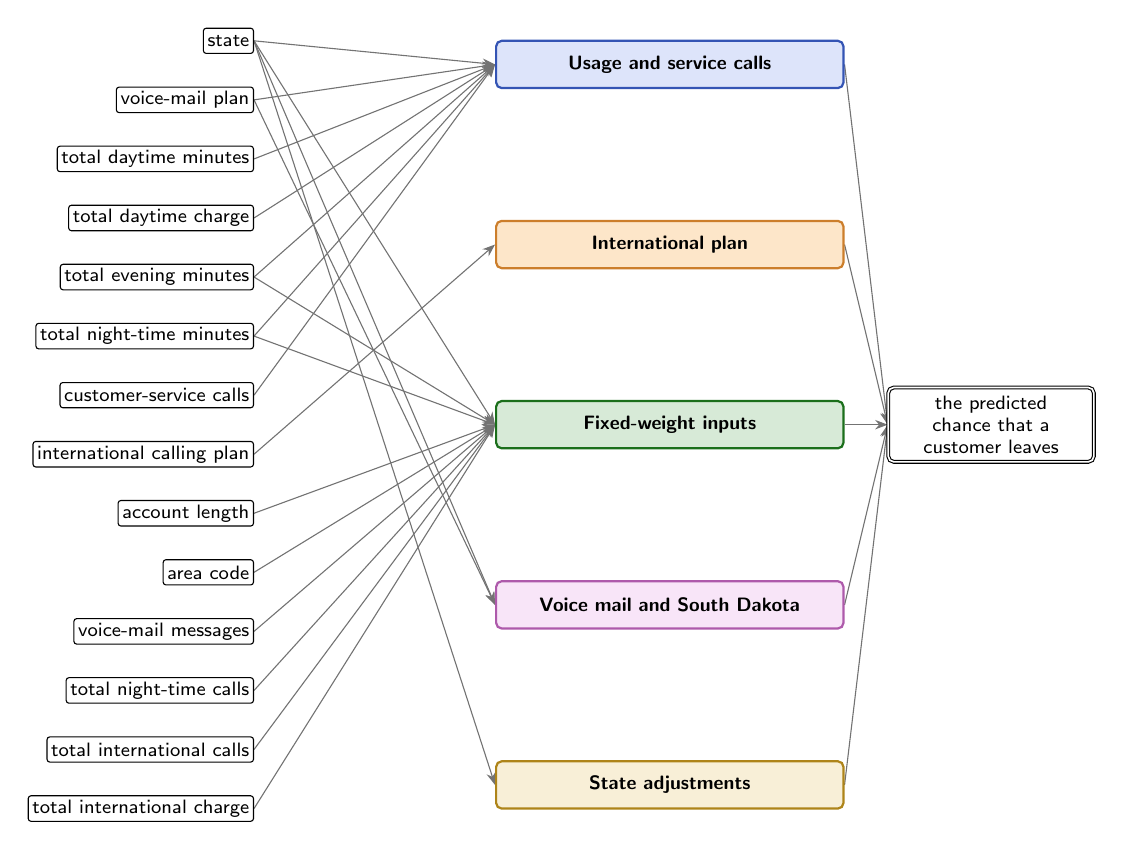
\begin{tikzpicture}[
  font=\sffamily\scriptsize, >={Stealth[length=1.6mm]},
  inp/.style={draw, rounded corners=1pt, fill=white, inner sep=1.5pt, minimum height=3.2mm, anchor=east},
  abox/.style={draw, thick, rounded corners=2pt, align=center, inner sep=3pt, minimum height=6mm, text width=42mm},
  outp/.style={draw, double, rounded corners=2pt, fill=white, align=center, inner sep=3pt, text width=24mm},
  agg/.style={draw=black!55},
]
\node[inp] (i0) at (0,4.875) {state};
\node[inp] (i1) at (0,4.125) {voice-mail plan};
\node[inp] (i2) at (0,3.375) {total daytime minutes};
\node[inp] (i3) at (0,2.625) {total daytime charge};
\node[inp] (i4) at (0,1.875) {total evening minutes};
\node[inp] (i5) at (0,1.125) {total night-time minutes};
\node[inp] (i6) at (0,0.375) {customer-service calls};
\node[inp] (i7) at (0,-0.375) {international calling plan};
\node[inp] (i8) at (0,-1.125) {account length};
\node[inp] (i9) at (0,-1.875) {area code};
\node[inp] (i10) at (0,-2.625) {voice-mail messages};
\node[inp] (i11) at (0,-3.375) {total night-time calls};
\node[inp] (i12) at (0,-4.125) {total international calls};
\node[inp] (i13) at (0,-4.875) {total international charge};
\node[abox, fill=RoyalBlue!18, draw=RoyalBlue!80!black] (b0) at (5.28,4.575) {\textbf{Usage and service calls}};
\node[abox, fill=BurntOrange!18, draw=BurntOrange!80!black] (b1) at (5.28,2.288) {\textbf{International plan}};
\node[abox, fill=ForestGreen!18, draw=ForestGreen!80!black] (b2) at (5.28,-0.0) {\textbf{Fixed-weight inputs}};
\node[abox, fill=Orchid!18, draw=Orchid!80!black] (b3) at (5.28,-2.288) {\textbf{Voice mail and South Dakota}};
\node[abox, fill=Goldenrod!18, draw=Goldenrod!80!black] (b4) at (5.28,-4.575) {\textbf{State adjustments}};
\node[outp] (out) at (9.36,0) {the predicted chance that a customer leaves};
\begin{scope}[on background layer]
\draw[->, agg, thin] (i0.east) -- (b0.west);
\draw[->, agg, thin] (i1.east) -- (b0.west);
\draw[->, agg, thin] (i2.east) -- (b0.west);
\draw[->, agg, thin] (i3.east) -- (b0.west);
\draw[->, agg, thin] (i4.east) -- (b0.west);
\draw[->, agg, thin] (i5.east) -- (b0.west);
\draw[->, agg, thin] (i6.east) -- (b0.west);
\draw[->, agg] (b0.east) -- (out.west);
\draw[->, agg, thin] (i7.east) -- (b1.west);
\draw[->, agg] (b1.east) -- (out.west);
\draw[->, agg, thin] (i0.east) -- (b2.west);
\draw[->, agg, thin] (i8.east) -- (b2.west);
\draw[->, agg, thin] (i9.east) -- (b2.west);
\draw[->, agg, thin] (i10.east) -- (b2.west);
\draw[->, agg, thin] (i4.east) -- (b2.west);
\draw[->, agg, thin] (i5.east) -- (b2.west);
\draw[->, agg, thin] (i11.east) -- (b2.west);
\draw[->, agg, thin] (i12.east) -- (b2.west);
\draw[->, agg, thin] (i13.east) -- (b2.west);
\draw[->, agg] (b2.east) -- (out.west);
\draw[->, agg, thin] (i0.east) -- (b3.west);
\draw[->, agg, thin] (i1.east) -- (b3.west);
\draw[->, agg] (b3.east) -- (out.west);
\draw[->, agg, thin] (i0.east) -- (b4.west);
\draw[->, agg] (b4.east) -- (out.west);
\end{scope}
\end{tikzpicture}}}%
\caption{The whole model: what feeds it, one level down.}
\label{fig:churn100s7c1:parts-ann84}
\end{figure}
\begin{figure}[H]\centering
\resizebox{\ifdim\width>\linewidth\linewidth\else\width\fi}{!}{%
\definecolor{netup}{HTML}{D95F02}\definecolor{netdown}{HTML}{1B9E77}\definecolor{netmixed}{HTML}{7F7F7F}%
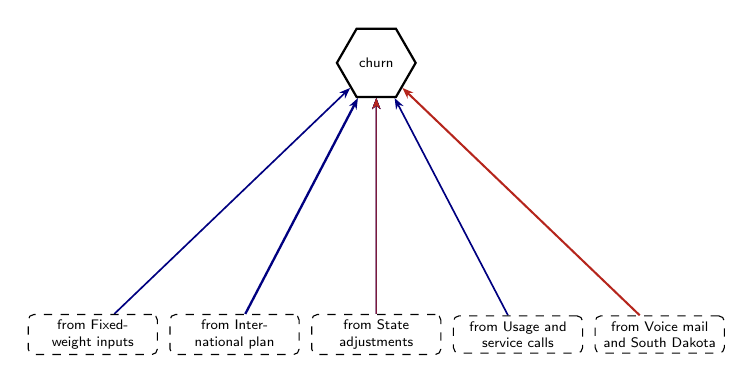
\begin{tikzpicture}[
  font=\sffamily\scriptsize, >={Stealth[length=1.4mm]},
  inp/.style={draw, circle, fill=white, minimum size=3.2mm, inner sep=0pt},
  hid/.style={draw, circle, fill=white, minimum size=5.2mm, inner sep=0.5pt, font=\sffamily\tiny},
  exitbox/.style={draw, thick, rectangle, fill=white, align=center, text width=17mm, minimum height=5mm, inner sep=1.5pt, font=\sffamily\tiny},
  sumbox/.style={draw, thick, dashed, rectangle, fill=white, align=center, text width=17mm, minimum height=5mm, inner sep=1.5pt, font=\sffamily\tiny},
  outp/.style={draw, thick, regular polygon, regular polygon sides=6, fill=white, minimum size=10mm, inner sep=0pt, font=\sffamily\tiny, align=center},
  stub/.style={draw, dashed, rounded corners=2pt, fill=white, align=center, inner sep=2pt, font=\sffamily\tiny, text width=15mm},
  inlab/.style={font=\sffamily\tiny, align=center, text width=15mm, inner sep=1pt, fill=white, fill opacity=0.8, text opacity=1},
  wpos/.style={draw=NavyBlue}, wneg/.style={draw=BrickRed}, wagg/.style={draw=black!45, line width=1.2pt},
  wmix/.style={draw=Plum},
]
\node[outp] (n0) at (4.5,3.45) {churn};
\node[stub] (nfromxxVoicexmailxandxSouthxDakota) at (8.1,0.0) {from Voice mail and South Dakota};
\node[stub] (nfromxxStatexadjustments) at (4.5,0.0) {from State adjustments};
\node[stub] (nfromxxInternationalxplan) at (2.7,0.0) {from International plan};
\node[stub] (nfromxxFixedmweightxinputs) at (0.9,0.0) {from Fixed-weight inputs};
\node[stub] (nfromxxUsagexandxservicexcalls) at (6.3,0.0) {from Usage and service calls};
\begin{scope}[on background layer]
\draw[->, wneg, line width=0.74pt] (nfromxxVoicexmailxandxSouthxDakota) -- (n0);
\draw[->, wneg, line width=0.34pt] (nfromxxStatexadjustments) -- (n0);
\draw[->, wpos, line width=0.26pt] (nfromxxStatexadjustments) -- (n0);
\draw[->, wneg, line width=0.28pt] (nfromxxStatexadjustments) -- (n0);
\draw[->, wpos, line width=0.84pt] (nfromxxInternationalxplan) -- (n0);
\draw[->, wpos, line width=0.26pt] (nfromxxStatexadjustments) -- (n0);
\draw[->, wpos, line width=0.30pt] (nfromxxStatexadjustments) -- (n0);
\draw[->, wneg, line width=0.29pt] (nfromxxStatexadjustments) -- (n0);
\draw[->, wpos, line width=0.60pt] (nfromxxFixedmweightxinputs) -- (n0);
\draw[->, wpos, line width=0.60pt] (nfromxxUsagexandxservicexcalls) -- (n0);
\end{scope}
\end{tikzpicture}}%
\caption{The whole model: its units and every connection into them. Blue: positive weight (raises the score); red: negative weight (lowers it); thicker: larger weight. Orange outline and up arrow: raises the final prediction; teal and down arrow: lowers it; grey and double arrow: depends.}
\label{fig:churn100s7c1:units-ann84}
\end{figure}
\paragraph{Hypothesis.} The model adds up five parts into one score: usage and service calls, the international plan, fixed-weight inputs, a voice-mail and South Dakota adjustment, and state adjustments.\,{\scriptsize\textcolor{NavyBlue}{[C047]}}
\paragraph{Evidence.} It is made up of these five parts (each explained below); the score is their sum, which was checked on all 4000 training customers.\,{\scriptsize\textcolor{NavyBlue}{[C047]}} Changing one input at a time across the whole model, an international plan takes a typical customer's chance of leaving from about 1\% to about 15\%, and more daytime minutes raise it in an uneven way, from about 1\% at 112 to about 4\% at 249 minutes.\,{\scriptsize\textcolor{NavyBlue}{[C001, C004]}} In Washington the chance is about 5\% and in Montana about 4\%, against about 1\% in West Virginia and under 1\% in Vermont.\,{\scriptsize\textcolor{NavyBlue}{[C002, C003, C022]}} The model ignores daytime calls, evening calls, the evening charge, international minutes and the night-time charge.\,{\scriptsize\textcolor{NavyBlue}{[C042, C043, C044, C045, C046]}}
\par\noindent{\small Evidence plots: Figure~\ref{fig:churn100s7c1:plot-ann84-0}, Figure~\ref{fig:churn100s7c1:plot-ann84-1}.\par}
\begin{figure}[H]\centering
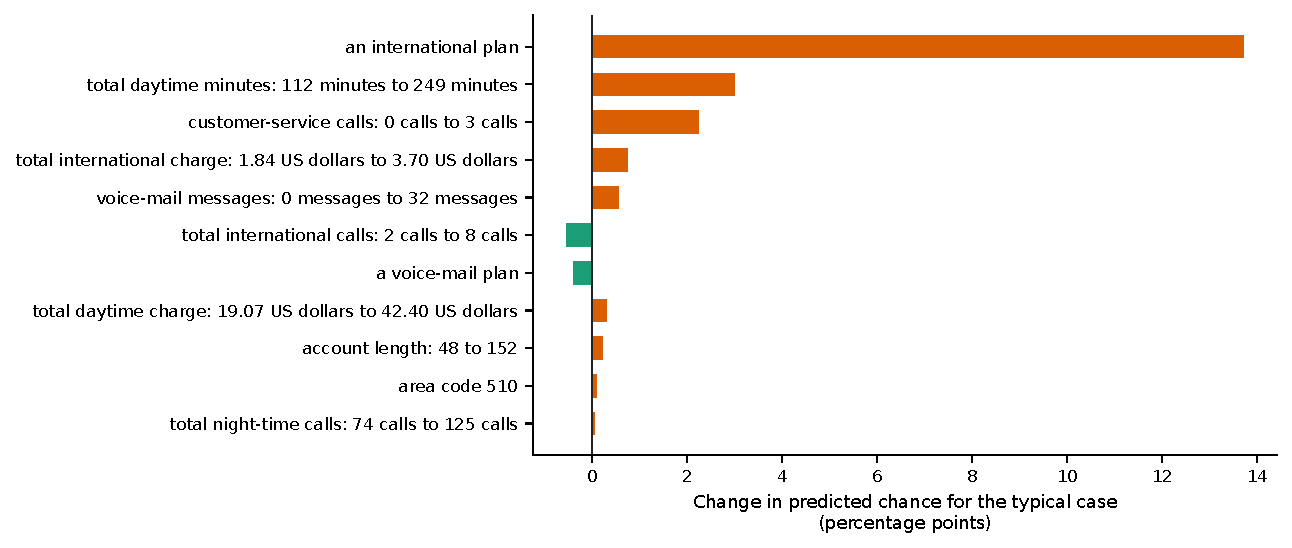
\includegraphics[width=\linewidth,height=0.88\textheight,keepaspectratio]{figures/churn100-s7-c1/ann_84-effects.pdf}
\caption{The whole model: Each input's change in the predicted value for the typical case across the whole model, largest first (orange: raises it, teal: lowers it).}
\label{fig:churn100s7c1:plot-ann84-0}
\end{figure}
\begin{figure}[H]\centering
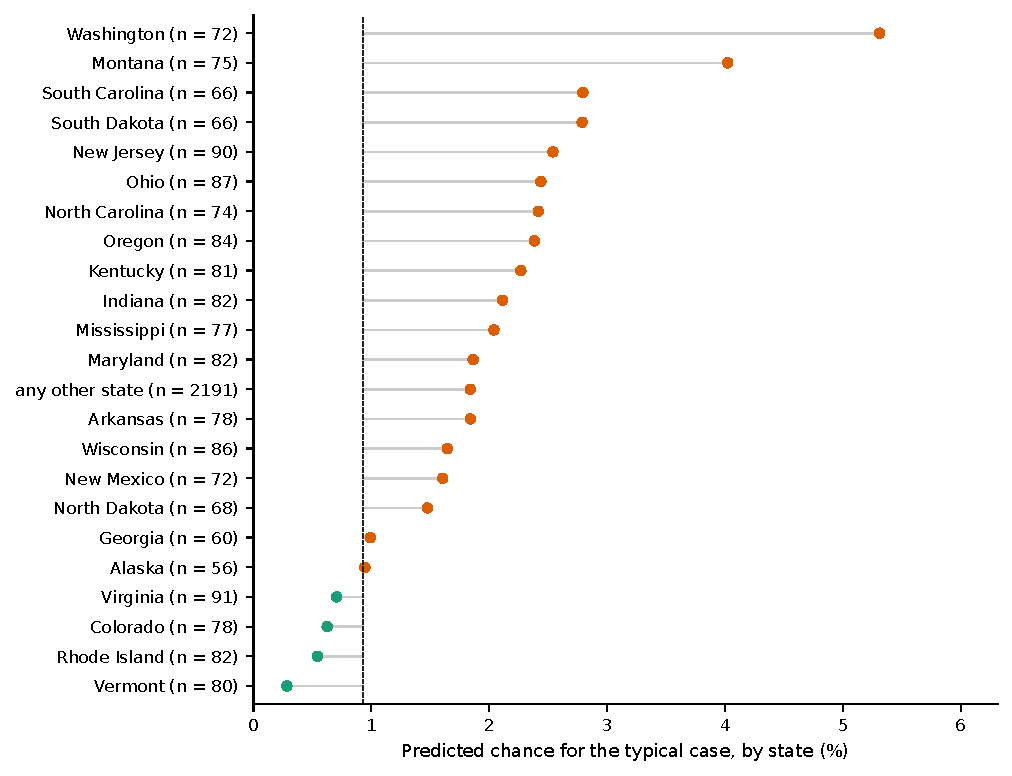
\includegraphics[width=\linewidth,height=0.88\textheight,keepaspectratio]{figures/churn100-s7-c1/ann_84-levels-state.pdf}
\caption{The whole model: Every level of state the model reads: the predicted value for the typical case at that level (dashed: the reference level); n = training customers; grey: few customers or not supported.}
\label{fig:churn100s7c1:plot-ann84-1}
\end{figure}
\par\smallskip\noindent{\small \textbf{Dive deeper:} Usage and service calls (\ref{rd:ann83}); International plan (\ref{rd:ann81}); Fixed-weight inputs (\ref{rd:ann78}); Voice mail and South Dakota (\ref{rd:ann80}); State adjustments (\ref{rd:ann82}). Technical detail: \ref{tech:ann84}.\par}
\subsubsection{Usage and service calls}\label{rd:ann83}
\noindent{\footnotesize Part of: The whole model (\ref{rd:ann84}).\par}
\noindent{\small Figure~\ref{fig:churn100s7c1:parts-ann83} shows what feeds this part; Figure~\ref{fig:churn100s7c1:units-ann83} its units and every connection into them (dashed boxes: connections from or to other parts, drawn in their own sections).\par}
\begin{figure}[H]\centering
\resizebox{!}{\ifdim\height>0.5\textheight 0.5\textheight\else\height\fi}{%
\resizebox{\ifdim\width>\linewidth\linewidth\else\width\fi}{!}{%
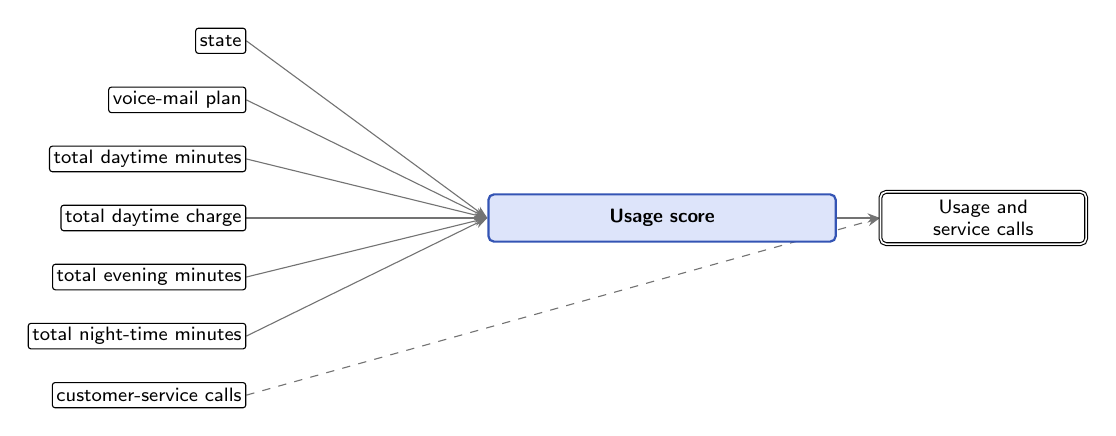
\begin{tikzpicture}[
  font=\sffamily\scriptsize, >={Stealth[length=1.6mm]},
  inp/.style={draw, rounded corners=1pt, fill=white, inner sep=1.5pt, minimum height=3.2mm, anchor=east},
  abox/.style={draw, thick, rounded corners=2pt, align=center, inner sep=3pt, minimum height=6mm, text width=42mm},
  outp/.style={draw, double, rounded corners=2pt, fill=white, align=center, inner sep=3pt, text width=24mm},
  agg/.style={draw=black!55},
]
\node[inp] (i0) at (0,2.25) {state};
\node[inp] (i1) at (0,1.5) {voice-mail plan};
\node[inp] (i2) at (0,0.75) {total daytime minutes};
\node[inp] (i3) at (0,-0.0) {total daytime charge};
\node[inp] (i4) at (0,-0.75) {total evening minutes};
\node[inp] (i5) at (0,-1.5) {total night-time minutes};
\node[inp] (i6) at (0,-2.25) {customer-service calls};
\node[abox, fill=RoyalBlue!18, draw=RoyalBlue!80!black] (b0) at (5.28,0.0) {\textbf{Usage score}};
\node[outp] (out) at (9.36,0) {Usage and service calls};
\begin{scope}[on background layer]
\draw[->, agg, thin] (i0.east) -- (b0.west);
\draw[->, agg, thin] (i1.east) -- (b0.west);
\draw[->, agg, thin] (i2.east) -- (b0.west);
\draw[->, agg, thin] (i3.east) -- (b0.west);
\draw[->, agg, thin] (i4.east) -- (b0.west);
\draw[->, agg, thin] (i5.east) -- (b0.west);
\draw[->, agg] (b0.east) -- (out.west);
\draw[->, agg, thin, dashed] (i6.east) -- (out.west);
\end{scope}
\end{tikzpicture}}}%
\caption{Usage and service calls: what feeds it, one level down.}
\label{fig:churn100s7c1:parts-ann83}
\end{figure}
\begin{figure}[H]\centering
\resizebox{\ifdim\width>\linewidth\linewidth\else\width\fi}{!}{%
\definecolor{netup}{HTML}{D95F02}\definecolor{netdown}{HTML}{1B9E77}\definecolor{netmixed}{HTML}{7F7F7F}%
\begin{tikzpicture}[
  font=\sffamily\scriptsize, >={Stealth[length=1.4mm]},
  inp/.style={draw, circle, fill=white, minimum size=3.2mm, inner sep=0pt},
  hid/.style={draw, circle, fill=white, minimum size=5.2mm, inner sep=0.5pt, font=\sffamily\tiny},
  exitbox/.style={draw, thick, rectangle, fill=white, align=center, text width=17mm, minimum height=5mm, inner sep=1.5pt, font=\sffamily\tiny},
  sumbox/.style={draw, thick, dashed, rectangle, fill=white, align=center, text width=17mm, minimum height=5mm, inner sep=1.5pt, font=\sffamily\tiny},
  outp/.style={draw, thick, regular polygon, regular polygon sides=6, fill=white, minimum size=10mm, inner sep=0pt, font=\sffamily\tiny, align=center},
  stub/.style={draw, dashed, rounded corners=2pt, fill=white, align=center, inner sep=2pt, font=\sffamily\tiny, text width=15mm},
  inlab/.style={font=\sffamily\tiny, align=center, text width=15mm, inner sep=1pt, fill=white, fill opacity=0.8, text opacity=1},
  wpos/.style={draw=NavyBlue}, wneg/.style={draw=BrickRed}, wagg/.style={draw=black!45, line width=1.2pt},
  wmix/.style={draw=Plum},
]
\node[hid] (n14351) at (1.55,1.9) {h14};
\node[exitbox] (nidentityxusage) at (2.3,4.6) {Usage and service calls $\uparrow$};
\node[hid] (n10552) at (2.3,3.25) {h10};
\node[hid] (n4344) at (3.05,1.9) {h5};
\node[inp, draw=netup, very thick] (ninxxnumberxcustomerxservicexcalls) at (3.2,0.0) {};
\path (ninxxnumberxcustomerxservicexcalls.south) node[inlab, anchor=north] (labninxxnumberxcustomerxservicexcalls) {customer-service calls $\uparrow$};
\node[stub] (nfromxxUsagexscore) at (1.4,0.0) {from Usage score};
\node[stub] (ntoxxthexmodelxoutput) at (2.3,6.15) {to the model output};
\begin{scope}[on background layer]
\node[fit=(n14351) (nidentityxusage) (n10552) (n4344) , inner sep=8pt, rounded corners=5pt, fill=BurntOrange!10, draw=BurntOrange!45] (clu0) {};
\draw[->, wpos, line width=0.51pt] (ninxxnumberxcustomerxservicexcalls) -- (n4344);
\draw[->, wneg, line width=1.38pt] (nfromxxUsagexscore) -- (n4344);
\draw[->, wpos, line width=0.63pt] (nfromxxUsagexscore) -- (n14351);
\draw[->, wpos, line width=0.66pt] (n14351) -- (n10552);
\draw[->, wpos, line width=1.15pt] (nfromxxUsagexscore) -- (nidentityxusage);
\draw[->, wpos, line width=1.26pt] (n4344) -- (nidentityxusage);
\draw[->, wpos, line width=1.32pt] (n10552) -- (nidentityxusage);
\draw[->, wpos, line width=0.60pt] (nidentityxusage) -- (ntoxxthexmodelxoutput);
\end{scope}
\node[font=\sffamily\scriptsize\bfseries, text=BurntOrange!55!black, anchor=south west, inner sep=1pt, fill=white, fill opacity=0.85, text opacity=1] at (clu0.north west) {Usage and service calls};
\end{tikzpicture}}%
\caption{Usage and service calls: its units and every connection into them. Blue: positive weight (raises the score); red: negative weight (lowers it); thicker: larger weight. Orange outline and up arrow: raises the final prediction; teal and down arrow: lowers it; grey and double arrow: depends.}
\label{fig:churn100s7c1:units-ann83}
\end{figure}
\paragraph{Hypothesis.} This part raises the chance of leaving for heavy daytime users without a voice-mail plan and for customers who call customer service 3 times or more: daytime minutes in an uneven way, and calls for most customers slowly at first, then faster, but for some customers without a voice-mail plan nothing until a point, then steadily.\,{\scriptsize\textcolor{NavyBlue}{[C056, C055]}}
\paragraph{Evidence.} It is made up of the usage score (explained below) together with customer-service calls, combined in a way that is not a simple sum.\,{\scriptsize\textcolor{NavyBlue}{[C060]}} Through it, daytime minutes add only above about 187 minutes for customers without a voice-mail plan, in an uneven way, from about 1\% to about 11\% between 0 and 271 minutes for a typical customer.\,{\scriptsize\textcolor{NavyBlue}{[C056]}} Customer-service calls add only from about 3 calls upwards, for most customers slowly at first, then faster, but for some customers without a voice-mail plan nothing until a point, then steadily, from about 1\% to about 15\% between 0 and 4 calls.\,{\scriptsize\textcolor{NavyBlue}{[C055]}}
\par\noindent{\small Evidence plots: Figure~\ref{fig:churn100s7c1:plot-ann83-0}, Figure~\ref{fig:churn100s7c1:plot-ann83-1}, Figure~\ref{fig:churn100s7c1:plot-ann83-2}, Figure~\ref{fig:churn100s7c1:plot-ann83-3}, Figure~\ref{fig:churn100s7c1:plot-ann83-4}, Figure~\ref{fig:churn100s7c1:plot-ann83-5}, Figure~\ref{fig:churn100s7c1:plot-ann83-6}.\par}
\par\noindent{\small Figure~\ref{fig:churn100s7c1:plot-ann83-5} shows this part's own output, unit h16: over its two main inputs, with the line where it switches on.\par}
\begin{figure}[H]\centering
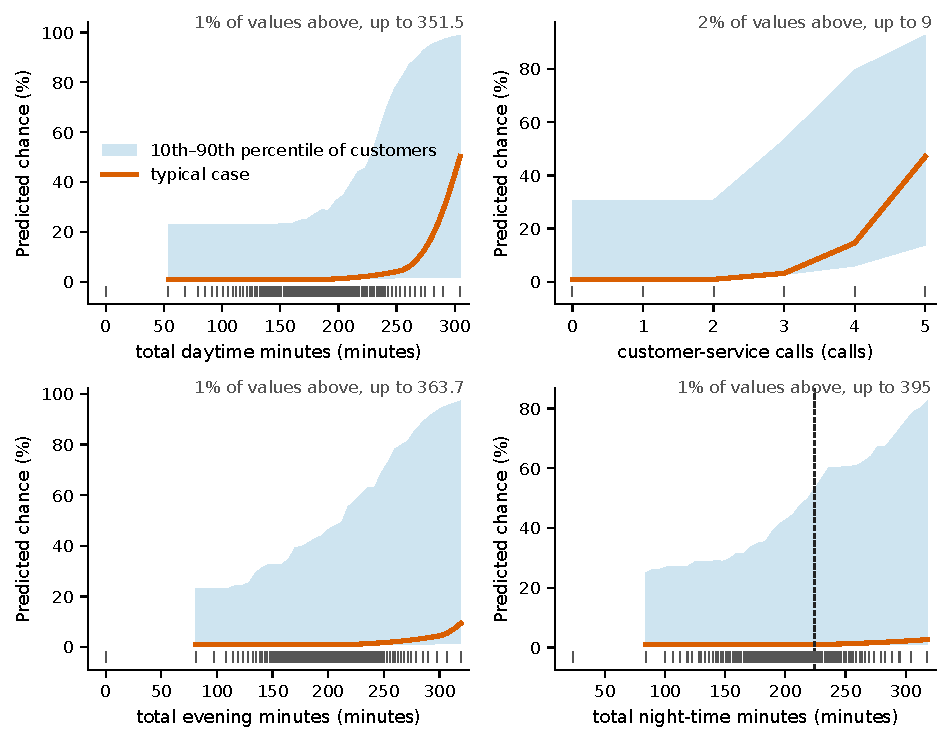
\includegraphics[width=\linewidth,height=0.88\textheight,keepaspectratio]{figures/churn100-s7-c1/ann_83-response.pdf}
\caption{Usage and service calls: Response curves through this part: the typical case (bold), the 10th to 90th percentile of individual customers (band), the fold or step point (dashed) with its spread across them (grey), and the observed values (ticks).}
\label{fig:churn100s7c1:plot-ann83-0}
\end{figure}
\begin{figure}[H]\centering
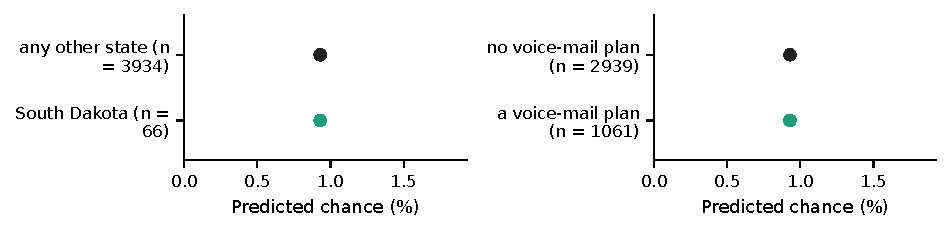
\includegraphics[width=\linewidth,height=0.88\textheight,keepaspectratio]{figures/churn100-s7-c1/ann_83-categories-small.pdf}
\caption{Usage and service calls: The predicted value for the typical case at each level, through this part (n = training customers; grey: fewer than 20).}
\label{fig:churn100s7c1:plot-ann83-1}
\end{figure}
\begin{figure}[H]\centering
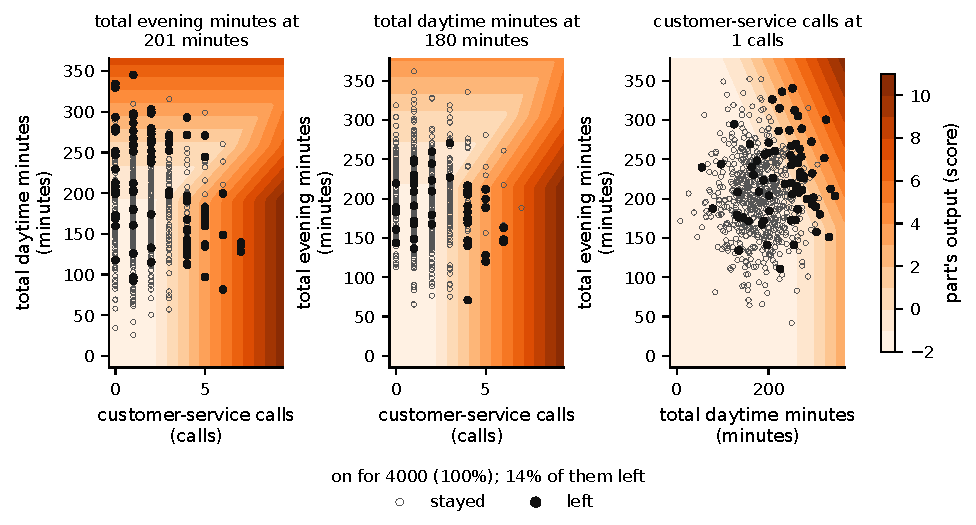
\includegraphics[width=\linewidth,height=0.88\textheight,keepaspectratio]{figures/churn100-s7-c1/ann_83-deep-map.pdf}
\caption{Usage and service calls: The part's own output over each pair of its three main inputs (the third held at its median, named above each panel; the points are the training rows whose third input is between its 40th and 60th percentile), other inputs at the typical case: colour where it is on, flat grey where it is switched off, the black line where it switches on; training customers as hollow (no event) and filled (event) points, so the part can be seen catching the events (the predicted-chance overlay was harder to read). The switch-on line is traced on this map only; the boundary claim (C118) did not pass its check on the data, so no rule is stated.}
\label{fig:churn100s7c1:plot-ann83-2}
\end{figure}
\begin{figure}[H]\centering
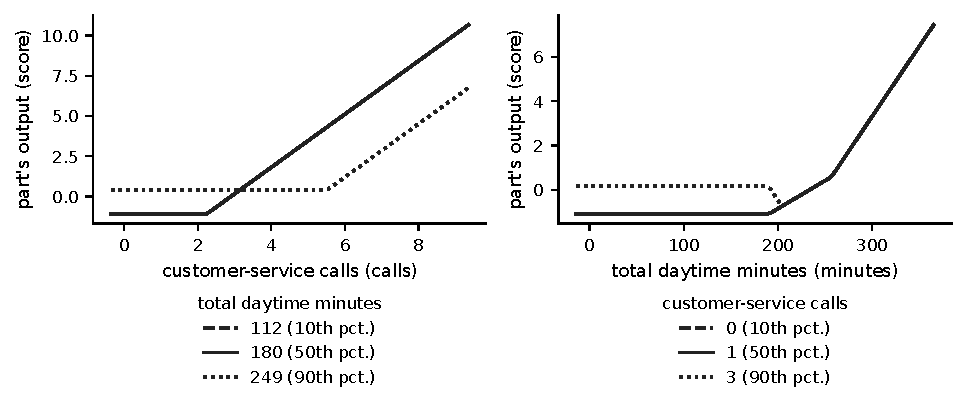
\includegraphics[width=\linewidth,height=0.88\textheight,keepaspectratio]{figures/churn100-s7-c1/ann_83-deep-slices.pdf}
\caption{Usage and service calls: Slices of the same map: the part's own output against each input at three values of the other, so the tilted boundary shows as a shifting hinge. The switch-on line is traced on this map only; the boundary claim (C118) did not pass its check on the data, so no rule is stated.}
\label{fig:churn100s7c1:plot-ann83-3}
\end{figure}
\begin{figure}[H]\centering
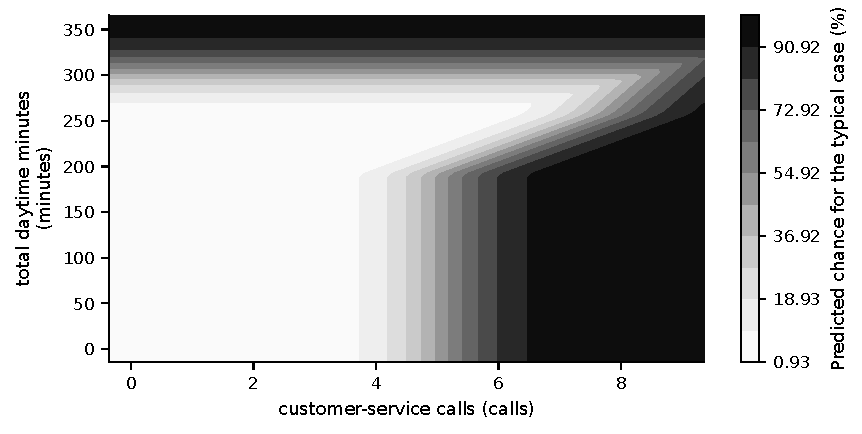
\includegraphics[width=\linewidth,height=0.88\textheight,keepaspectratio]{figures/churn100-s7-c1/ann_83-deep-risk.pdf}
\caption{Usage and service calls: The same map on the final scale: the predicted value for the typical case, with the switch-on line (orange). The switch-on line is traced on this map only; the boundary claim (C118) did not pass its check on the data, so no rule is stated.}
\label{fig:churn100s7c1:plot-ann83-4}
\end{figure}
\begin{figure}[H]\centering
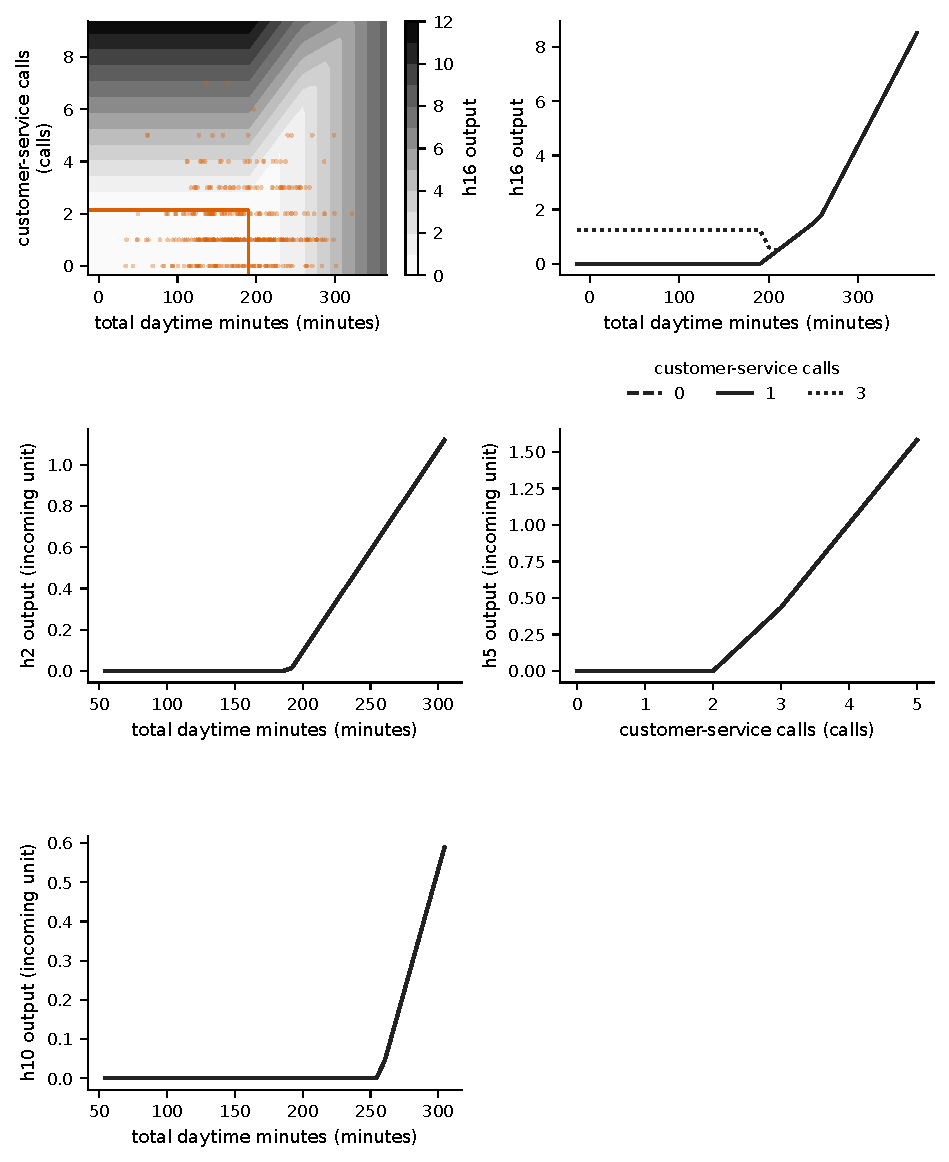
\includegraphics[width=\linewidth,height=0.88\textheight,keepaspectratio]{figures/churn100-s7-c1/ann_83-partial-identity_usage.pdf}
\caption{Usage and service calls: This part's own output, unit h16 (combines 3 non-linear units), on its own scale (its activation), with every other input at the typical case; it is active for 1927 of 4000. Left: its output over its two main inputs (orange line: where it switches on; dots: the data); right: slices at three values of the second input; then each incoming non-linear unit against its own main input.}
\label{fig:churn100s7c1:plot-ann83-5}
\end{figure}
\begin{figure}[H]\centering
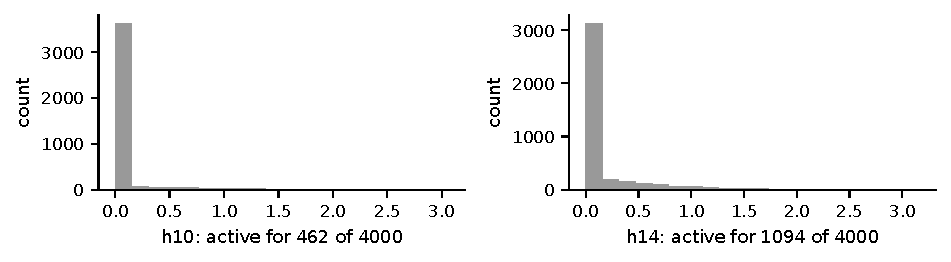
\includegraphics[width=\linewidth,height=0.88\textheight,keepaspectratio]{figures/churn100-s7-c1/ann_83-units.pdf}
\caption{Usage and service calls: This part's hidden units: each unit's output against its main numeric input (top) and how often it is active (bottom).}
\label{fig:churn100s7c1:plot-ann83-6}
\end{figure}
\par\smallskip\noindent{\small \textbf{Dive deeper:} Usage score (\ref{rd:ann79}). Technical detail: \ref{tech:ann83}.\par}
\subsubsection{Usage score}\label{rd:ann79}
\noindent{\footnotesize Part of: Usage and service calls (\ref{rd:ann83}).\par}
\noindent{\small Figure~\ref{fig:churn100s7c1:parts-ann79} shows what feeds this part; Figure~\ref{fig:churn100s7c1:units-ann79} its units and every connection into them (dashed boxes: connections from or to other parts, drawn in their own sections).\par}
\begin{figure}[H]\centering
\resizebox{!}{\ifdim\height>0.5\textheight 0.5\textheight\else\height\fi}{%
\resizebox{\ifdim\width>\linewidth\linewidth\else\width\fi}{!}{%
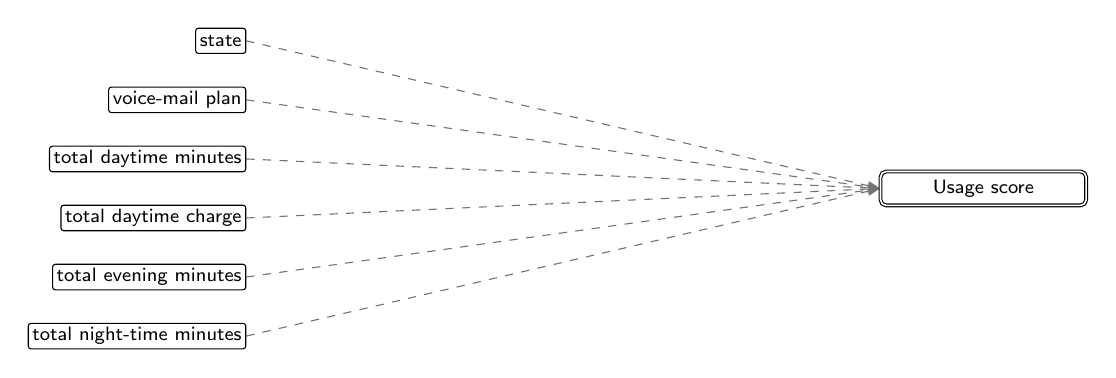
\begin{tikzpicture}[
  font=\sffamily\scriptsize, >={Stealth[length=1.6mm]},
  inp/.style={draw, rounded corners=1pt, fill=white, inner sep=1.5pt, minimum height=3.2mm, anchor=east},
  abox/.style={draw, thick, rounded corners=2pt, align=center, inner sep=3pt, minimum height=6mm, text width=42mm},
  outp/.style={draw, double, rounded corners=2pt, fill=white, align=center, inner sep=3pt, text width=24mm},
  agg/.style={draw=black!55},
]
\node[inp] (i0) at (0,1.875) {state};
\node[inp] (i1) at (0,1.125) {voice-mail plan};
\node[inp] (i2) at (0,0.375) {total daytime minutes};
\node[inp] (i3) at (0,-0.375) {total daytime charge};
\node[inp] (i4) at (0,-1.125) {total evening minutes};
\node[inp] (i5) at (0,-1.875) {total night-time minutes};
\node[outp] (out) at (9.36,0) {Usage score};
\begin{scope}[on background layer]
\draw[->, agg, thin, dashed] (i0.east) -- (out.west);
\draw[->, agg, thin, dashed] (i1.east) -- (out.west);
\draw[->, agg, thin, dashed] (i2.east) -- (out.west);
\draw[->, agg, thin, dashed] (i3.east) -- (out.west);
\draw[->, agg, thin, dashed] (i4.east) -- (out.west);
\draw[->, agg, thin, dashed] (i5.east) -- (out.west);
\end{scope}
\end{tikzpicture}}}%
\caption{Usage score: what feeds it, one level down.}
\label{fig:churn100s7c1:parts-ann79}
\end{figure}
\begin{figure}[H]\centering
\resizebox{\ifdim\width>\linewidth\linewidth\else\width\fi}{!}{%
\definecolor{netup}{HTML}{D95F02}\definecolor{netdown}{HTML}{1B9E77}\definecolor{netmixed}{HTML}{7F7F7F}%
\begin{tikzpicture}[
  font=\sffamily\scriptsize, >={Stealth[length=1.4mm]},
  inp/.style={draw, circle, fill=white, minimum size=3.2mm, inner sep=0pt},
  hid/.style={draw, circle, fill=white, minimum size=5.2mm, inner sep=0.5pt, font=\sffamily\tiny},
  exitbox/.style={draw, thick, rectangle, fill=white, align=center, text width=17mm, minimum height=5mm, inner sep=1.5pt, font=\sffamily\tiny},
  sumbox/.style={draw, thick, dashed, rectangle, fill=white, align=center, text width=17mm, minimum height=5mm, inner sep=1.5pt, font=\sffamily\tiny},
  outp/.style={draw, thick, regular polygon, regular polygon sides=6, fill=white, minimum size=10mm, inner sep=0pt, font=\sffamily\tiny, align=center},
  stub/.style={draw, dashed, rounded corners=2pt, fill=white, align=center, inner sep=2pt, font=\sffamily\tiny, text width=15mm},
  inlab/.style={font=\sffamily\tiny, align=center, text width=15mm, inner sep=1pt, fill=white, fill opacity=0.8, text opacity=1},
  wpos/.style={draw=NavyBlue}, wneg/.style={draw=BrickRed}, wagg/.style={draw=black!45, line width=1.2pt},
  wmix/.style={draw=Plum},
]
\node[hid] (n1406) at (5.4,1.9) {h3};
\node[hid] (n7558) at (5.4,3.25) {h9};
\node[exitbox] (n879) at (5.4,4.6) {Usage score $\updownarrow$};
\node[inp, draw=netup, very thick] (ninxxtotalxdayxminutes) at (6.3,0.0) {};
\path (ninxxtotalxdayxminutes.south) node[inlab, anchor=north] (labninxxtotalxdayxminutes) {total daytime minutes $\uparrow$};
\node[inp, draw=netup, very thick] (ninxxtotalxdayxcharge) at (4.5,0.0) {};
\path (ninxxtotalxdayxcharge.south) node[inlab, anchor=north] (labninxxtotalxdayxcharge) {total daytime charge $\uparrow$};
\node[inp, draw=netmixed, very thick] (ngrpxxstate) at (2.7,0.0) {};
\path (ngrpxxstate.south) node[inlab, anchor=north] (labngrpxxstate) {state (23 of 51 used) $\updownarrow$};
\node[inp, draw=netdown, very thick] (ninxxvoicexmailxplan) at (0.9,0.0) {};
\path (ninxxvoicexmailxplan.south) node[inlab, anchor=north] (labninxxvoicexmailxplan) {a voice-mail plan $\downarrow$};
\node[inp, draw=netup, very thick] (ninxxtotalxevexminutes) at (8.1,0.0) {};
\path (ninxxtotalxevexminutes.south) node[inlab, anchor=north] (labninxxtotalxevexminutes) {total evening minutes $\uparrow$};
\node[inp, draw=netup, very thick] (ninxxtotalxnightxminutes) at (9.9,0.0) {};
\path (ninxxtotalxnightxminutes.south) node[inlab, anchor=north] (labninxxtotalxnightxminutes) {total night-time minutes $\uparrow$};
\node[stub] (ntoxxUsagexandxservicexcalls) at (5.4,6.15) {to Usage and service calls};
\begin{scope}[on background layer]
\node[fit=(n1406) (n7558) (n879) , inner sep=8pt, rounded corners=5pt, fill=BurntOrange!10, draw=BurntOrange!45] (clu0) {};
\draw[->, wpos, line width=0.43pt] (ninxxtotalxdayxminutes) -- (n879);
\draw[->, wpos, line width=0.44pt] (ninxxtotalxdayxcharge) -- (n1406);
\draw[->, wpos, line width=0.44pt] (n7558) -- (n879);
\draw[->, wpos, line width=0.67pt] (n1406) -- (n7558);
\draw[->, wneg, line width=0.60pt] (ninxxvoicexmailxplan) -- (n879);
\draw[->, wpos, line width=0.48pt] (ninxxtotalxevexminutes) -- (n7558);
\draw[->, wpos, line width=0.33pt] (ninxxtotalxnightxminutes) -- (n879);
\draw[->, wneg, line width=1.38pt] (n879) -- (ntoxxUsagexandxservicexcalls);
\draw[->, wpos, line width=0.63pt] (n879) -- (ntoxxUsagexandxservicexcalls);
\draw[->, wpos, line width=1.15pt] (n879) -- (ntoxxUsagexandxservicexcalls);
\draw[->, wneg, line width=0.56pt] (ngrpxxstate) -- node[pos=0.8, sloped, above, font=\sffamily\tiny, inner sep=1pt, fill=white, fill opacity=0.8, text opacity=1] {-0.88} (n1406);
\end{scope}
\node[font=\sffamily\scriptsize\bfseries, text=BurntOrange!55!black, anchor=south west, inner sep=1pt, fill=white, fill opacity=0.85, text opacity=1] at (clu0.north west) {Usage score};
\end{tikzpicture}}%
\caption{Usage score: its units and every connection into them. Blue: positive weight (raises the score); red: negative weight (lowers it); thicker: larger weight. Orange outline and up arrow: raises the final prediction; teal and down arrow: lowers it; grey and double arrow: depends.}
\label{fig:churn100s7c1:units-ann79}
\end{figure}
\paragraph{Hypothesis.} This part builds a usage score: heavy daytime use raises the chance of leaving, in an uneven way and more so with high evening minutes, and a voice-mail plan lowers it.\,{\scriptsize\textcolor{NavyBlue}{[C071, C067, C062]}}
\paragraph{Evidence.} Through it, daytime minutes add only above about 187 minutes for customers without a voice-mail plan, in an uneven way, from about 1\% to about 11\% between 0 and 271 minutes.\,{\scriptsize\textcolor{NavyBlue}{[C071]}} Daytime minutes count more with more than 201 evening minutes (about 1\% to about 11\%, against about 1\% to about 2\%) and with more than 200 night-time minutes (about 1\% to about 7\%, against about 1\% to about 3\%), in an uneven way.\,{\scriptsize\textcolor{NavyBlue}{[C067, C068]}} A voice-mail plan lowers the chance through it from about 3\% to about 1\% for the typical customer it acts on.\,{\scriptsize\textcolor{NavyBlue}{[C062]}} Its formula reproduces the part exactly on all 4000 training customers.\,{\scriptsize\textcolor{NavyBlue}{[C076]}}
\par\noindent{\small Evidence plots: Figure~\ref{fig:churn100s7c1:plot-ann79-0}, Figure~\ref{fig:churn100s7c1:plot-ann79-1}, Figure~\ref{fig:churn100s7c1:plot-ann79-2}, Figure~\ref{fig:churn100s7c1:plot-ann79-3}, Figure~\ref{fig:churn100s7c1:plot-ann79-4}, Figure~\ref{fig:churn100s7c1:plot-ann79-5}, Figure~\ref{fig:churn100s7c1:plot-ann79-6}, Figure~\ref{fig:churn100s7c1:plot-ann79-7}.\par}
\par\medskip\noindent\textbf{Worked example: reading this part.} Figure~\ref{fig:churn100s7c1:plot-ann79-3} maps the part's own output over its main inputs. In the grey region it is switched off and adds nothing; past the black line it switches on, and the colour shows how much it adds to the score. The line is the rule in the claim (C119): it switches on when total daytime minutes above about 220 (for total evening minutes from about 0.00 to 164); total daytime minutes plus about 0.75 $\times$ total evening minutes above about 341 (for total evening minutes from about 164 to 364). 1382 of 4000 training customers lie on the 'on' side, and 23\% of them left, against 10\% of the others: the filled points crowd on the 'on' side. Figure~\ref{fig:churn100s7c1:plot-ann79-4} cuts the map into slices: the hinge moves as the other input changes, which is what a tilted line means. Figure~\ref{fig:churn100s7c1:plot-ann79-5} shows what this does to the final prediction for the typical case.\par
\par\noindent{\small Figure~\ref{fig:churn100s7c1:plot-ann79-6} shows this part's own output, unit h2: over its two main inputs, with the line where it switches on.\par}
\begin{figure}[H]\centering
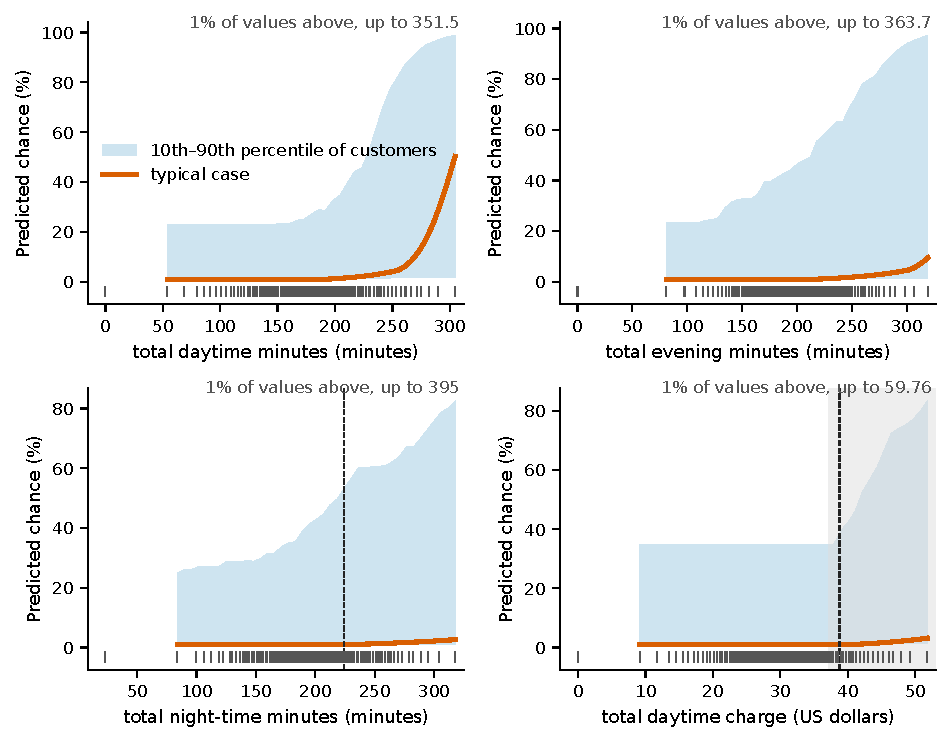
\includegraphics[width=\linewidth,height=0.88\textheight,keepaspectratio]{figures/churn100-s7-c1/ann_79-response.pdf}
\caption{Usage score: Response curves through this part: the typical case (bold), the 10th to 90th percentile of individual customers (band), the fold or step point (dashed) with its spread across them (grey), and the observed values (ticks).}
\label{fig:churn100s7c1:plot-ann79-0}
\end{figure}
\begin{figure}[H]\centering
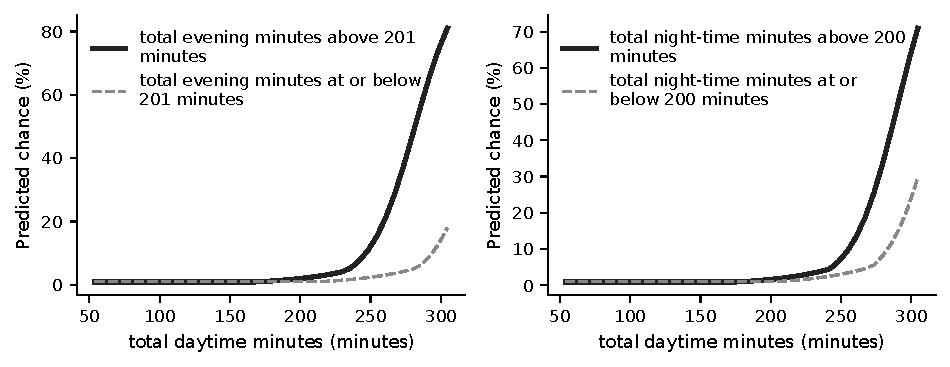
\includegraphics[width=\linewidth,height=0.88\textheight,keepaspectratio]{figures/churn100-s7-c1/ann_79-interaction.pdf}
\caption{Usage score: How the effect differs between groups: one curve per group, for the typical case of each group.}
\label{fig:churn100s7c1:plot-ann79-1}
\end{figure}
\begin{figure}[H]\centering
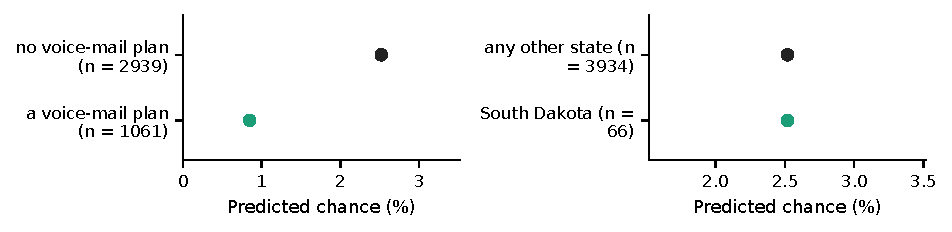
\includegraphics[width=\linewidth,height=0.88\textheight,keepaspectratio]{figures/churn100-s7-c1/ann_79-categories-small.pdf}
\caption{Usage score: The predicted value for the typical case at each level, through this part (n = training customers; grey: fewer than 20).}
\label{fig:churn100s7c1:plot-ann79-2}
\end{figure}
\begin{figure}[H]\centering
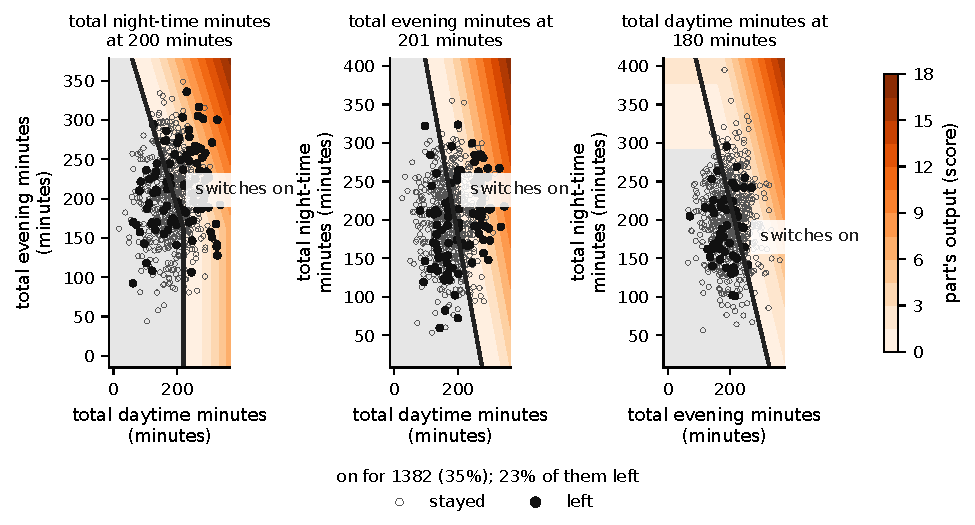
\includegraphics[width=\linewidth,height=0.88\textheight,keepaspectratio]{figures/churn100-s7-c1/ann_79-deep-map.pdf}
\caption{Usage score: The part's own output over each pair of its three main inputs (the third held at its median, named above each panel; the points are the training rows whose third input is between its 40th and 60th percentile), other inputs at the typical case: colour where it is on, flat grey where it is switched off, the black line where it switches on; training customers as hollow (no event) and filled (event) points, so the part can be seen catching the events (the predicted-chance overlay was harder to read).}
\label{fig:churn100s7c1:plot-ann79-3}
\end{figure}
\begin{figure}[H]\centering
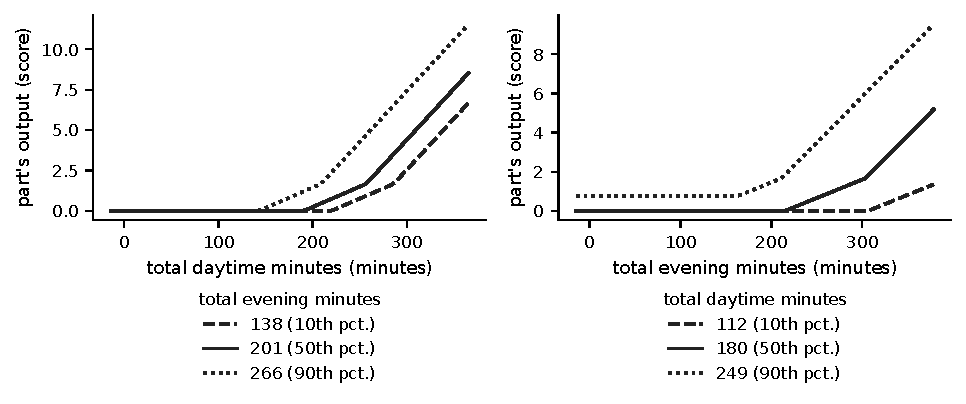
\includegraphics[width=\linewidth,height=0.88\textheight,keepaspectratio]{figures/churn100-s7-c1/ann_79-deep-slices.pdf}
\caption{Usage score: Slices of the same map: the part's own output against each input at three values of the other, so the tilted boundary shows as a shifting hinge.}
\label{fig:churn100s7c1:plot-ann79-4}
\end{figure}
\begin{figure}[H]\centering
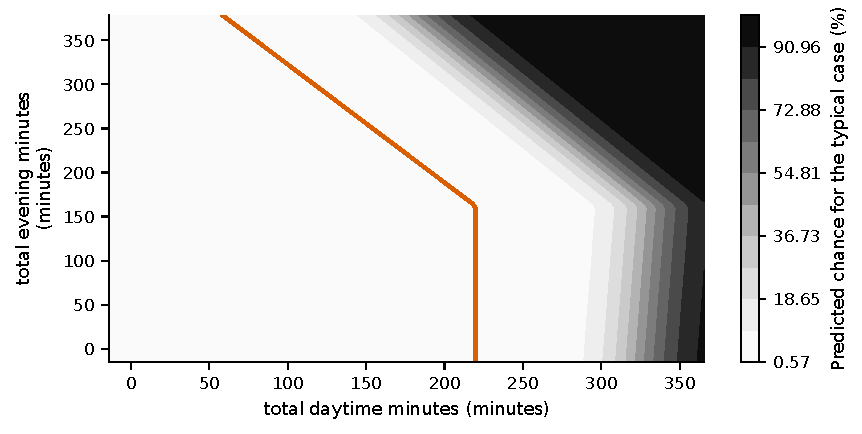
\includegraphics[width=\linewidth,height=0.88\textheight,keepaspectratio]{figures/churn100-s7-c1/ann_79-deep-risk.pdf}
\caption{Usage score: The same map on the final scale: the predicted value for the typical case, with the switch-on line (orange).}
\label{fig:churn100s7c1:plot-ann79-5}
\end{figure}
\begin{figure}[H]\centering
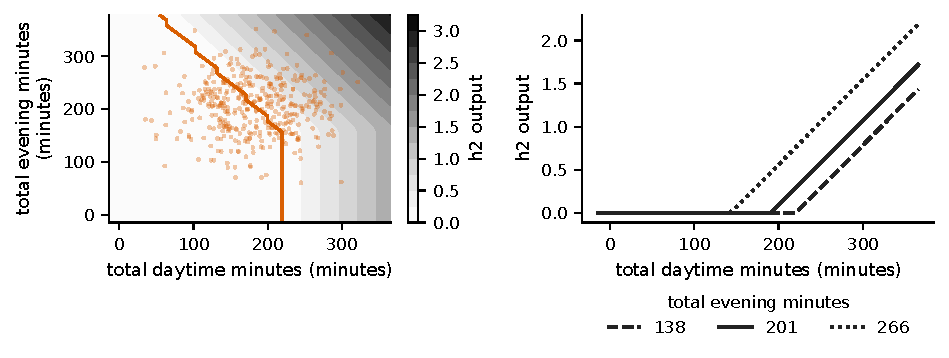
\includegraphics[width=\linewidth,height=0.88\textheight,keepaspectratio]{figures/churn100-s7-c1/ann_79-partial-879.pdf}
\caption{Usage score: This part's own output, unit h2 (the output of 'Usage score'), on its own scale (its activation), with every other input at the typical case; it is active for 1382 of 4000. Left: its output over its two main inputs (orange line: where it switches on; dots: the data); right: slices at three values of the second input.}
\label{fig:churn100s7c1:plot-ann79-6}
\end{figure}
\begin{figure}[H]\centering
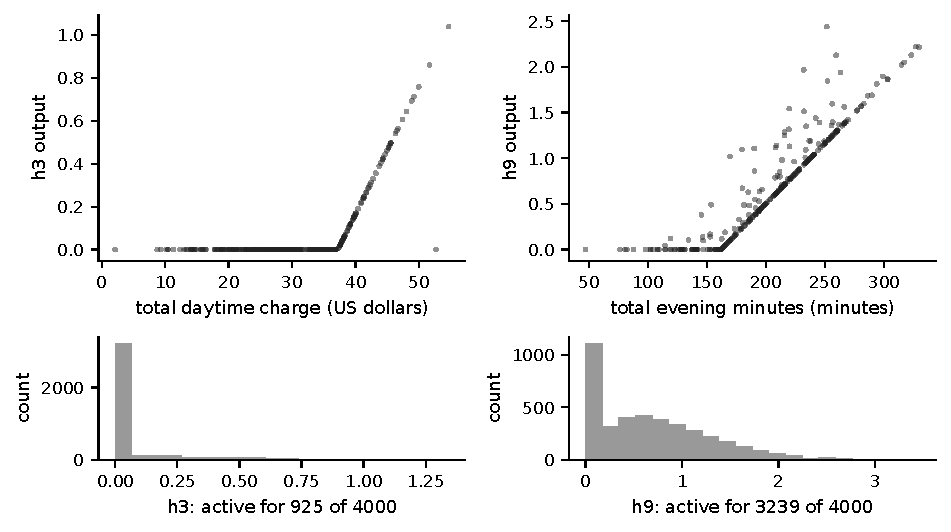
\includegraphics[width=\linewidth,height=0.88\textheight,keepaspectratio]{figures/churn100-s7-c1/ann_79-units.pdf}
\caption{Usage score: This part's hidden units: each unit's output against its main numeric input (top) and how often it is active (bottom).}
\label{fig:churn100s7c1:plot-ann79-7}
\end{figure}
\par\smallskip\noindent{\small Technical detail: \ref{tech:ann79}.\par}
\subsubsection{International plan}\label{rd:ann81}
\noindent{\footnotesize Part of: The whole model (\ref{rd:ann84}).\par}
\noindent{\small Figure~\ref{fig:churn100s7c1:parts-ann81} shows what feeds this part; Figure~\ref{fig:churn100s7c1:units-ann81} its units and every connection into them (dashed boxes: connections from or to other parts, drawn in their own sections).\par}
\begin{figure}[H]\centering
\resizebox{!}{\ifdim\height>0.5\textheight 0.5\textheight\else\height\fi}{%
\resizebox{\ifdim\width>\linewidth\linewidth\else\width\fi}{!}{%
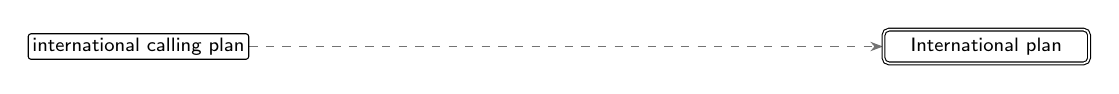
\begin{tikzpicture}[
  font=\sffamily\scriptsize, >={Stealth[length=1.6mm]},
  inp/.style={draw, rounded corners=1pt, fill=white, inner sep=1.5pt, minimum height=3.2mm, anchor=east},
  abox/.style={draw, thick, rounded corners=2pt, align=center, inner sep=3pt, minimum height=6mm, text width=42mm},
  outp/.style={draw, double, rounded corners=2pt, fill=white, align=center, inner sep=3pt, text width=24mm},
  agg/.style={draw=black!55},
]
\node[inp] (i0) at (0,-0.0) {international calling plan};
\node[outp] (out) at (9.36,0) {International plan};
\begin{scope}[on background layer]
\draw[->, agg, thin, dashed] (i0.east) -- (out.west);
\end{scope}
\end{tikzpicture}}}%
\caption{International plan: what feeds it, one level down.}
\label{fig:churn100s7c1:parts-ann81}
\end{figure}
\begin{figure}[H]\centering
\resizebox{\ifdim\width>\linewidth\linewidth\else\width\fi}{!}{%
\definecolor{netup}{HTML}{D95F02}\definecolor{netdown}{HTML}{1B9E77}\definecolor{netmixed}{HTML}{7F7F7F}%
\begin{tikzpicture}[
  font=\sffamily\scriptsize, >={Stealth[length=1.4mm]},
  inp/.style={draw, circle, fill=white, minimum size=3.2mm, inner sep=0pt},
  hid/.style={draw, circle, fill=white, minimum size=5.2mm, inner sep=0.5pt, font=\sffamily\tiny},
  exitbox/.style={draw, thick, rectangle, fill=white, align=center, text width=17mm, minimum height=5mm, inner sep=1.5pt, font=\sffamily\tiny},
  sumbox/.style={draw, thick, dashed, rectangle, fill=white, align=center, text width=17mm, minimum height=5mm, inner sep=1.5pt, font=\sffamily\tiny},
  outp/.style={draw, thick, regular polygon, regular polygon sides=6, fill=white, minimum size=10mm, inner sep=0pt, font=\sffamily\tiny, align=center},
  stub/.style={draw, dashed, rounded corners=2pt, fill=white, align=center, inner sep=2pt, font=\sffamily\tiny, text width=15mm},
  inlab/.style={font=\sffamily\tiny, align=center, text width=15mm, inner sep=1pt, fill=white, fill opacity=0.8, text opacity=1},
  wpos/.style={draw=NavyBlue}, wneg/.style={draw=BrickRed}, wagg/.style={draw=black!45, line width=1.2pt},
  wmix/.style={draw=Plum},
]
\node[exitbox] (n6711) at (1.8,1.9) {International plan $\uparrow$};
\node[inp, draw=netup, very thick] (ninxxinternationalxplan) at (1.8,0.0) {};
\path (ninxxinternationalxplan.south) node[inlab, anchor=north] (labninxxinternationalxplan) {an international plan $\uparrow$};
\node[stub] (ntoxxthexmodelxoutput) at (1.8,3.45) {to the model output};
\begin{scope}[on background layer]
\node[fit=(n6711) , inner sep=8pt, rounded corners=5pt, fill=ForestGreen!10, draw=ForestGreen!45] (clu0) {};
\draw[->, wpos, line width=0.47pt] (ninxxinternationalxplan) -- (n6711);
\draw[->, wpos, line width=0.84pt] (n6711) -- (ntoxxthexmodelxoutput);
\end{scope}
\node[font=\sffamily\scriptsize\bfseries, text=ForestGreen!55!black, anchor=south west, inner sep=1pt, fill=white, fill opacity=0.85, text opacity=1] at (clu0.north west) {International plan};
\end{tikzpicture}}%
\caption{International plan: its units and every connection into them. Blue: positive weight (raises the score); red: negative weight (lowers it); thicker: larger weight. Orange outline and up arrow: raises the final prediction; teal and down arrow: lowers it; grey and double arrow: depends.}
\label{fig:churn100s7c1:units-ann81}
\end{figure}
\paragraph{Hypothesis.} This part raises the chance of leaving for customers with an international plan.\,{\scriptsize\textcolor{NavyBlue}{[C077]}}
\paragraph{Evidence.} It acts on the 380 of 4000 training customers with an international plan, 161 of whom left; for the typical customer it acts on, the chance is about 2\% without it and about 26\% with it.\,{\scriptsize\textcolor{NavyBlue}{[C078]}} For a typical customer, an international plan takes the chance from about 1\% to about 15\%.\,{\scriptsize\textcolor{NavyBlue}{[C077]}} Its formula reproduces the part exactly on all 4000 training customers.\,{\scriptsize\textcolor{NavyBlue}{[C079]}}
\par\noindent{\small Evidence plots: Figure~\ref{fig:churn100s7c1:plot-ann81-0}, Figure~\ref{fig:churn100s7c1:plot-ann81-1}.\par}
\begin{figure}[H]\centering
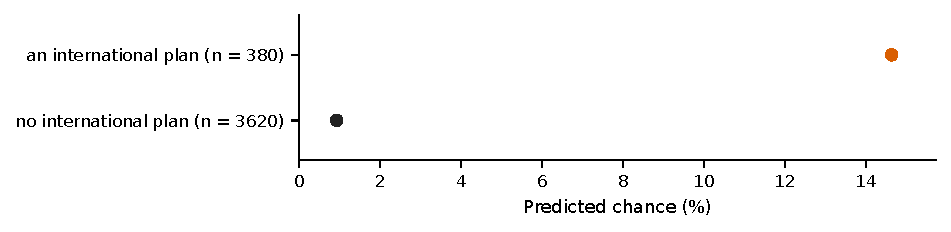
\includegraphics[width=\linewidth,height=0.88\textheight,keepaspectratio]{figures/churn100-s7-c1/ann_81-categories-small.pdf}
\caption{International plan: The predicted value for the typical case at each level, through this part (n = training customers; grey: fewer than 20).}
\label{fig:churn100s7c1:plot-ann81-0}
\end{figure}
\begin{figure}[H]\centering
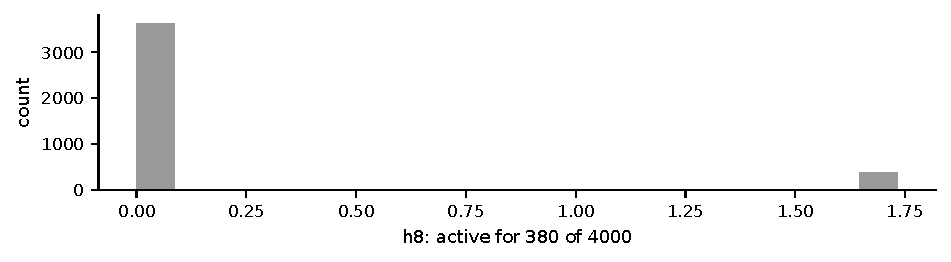
\includegraphics[width=\linewidth,height=0.88\textheight,keepaspectratio]{figures/churn100-s7-c1/ann_81-units.pdf}
\caption{International plan: This part's hidden units: each unit's output against its main numeric input (top) and how often it is active (bottom).}
\label{fig:churn100s7c1:plot-ann81-1}
\end{figure}
\par\smallskip\noindent{\small Technical detail: \ref{tech:ann81}.\par}
\subsubsection{Fixed-weight inputs}\label{rd:ann78}
\noindent{\footnotesize Part of: The whole model (\ref{rd:ann84}).\par}
\noindent{\small Figure~\ref{fig:churn100s7c1:parts-ann78} shows what feeds this part; Figure~\ref{fig:churn100s7c1:units-ann78} its units and every connection into them (dashed boxes: connections from or to other parts, drawn in their own sections).\par}
\begin{figure}[H]\centering
\resizebox{!}{\ifdim\height>0.5\textheight 0.5\textheight\else\height\fi}{%
\resizebox{\ifdim\width>\linewidth\linewidth\else\width\fi}{!}{%
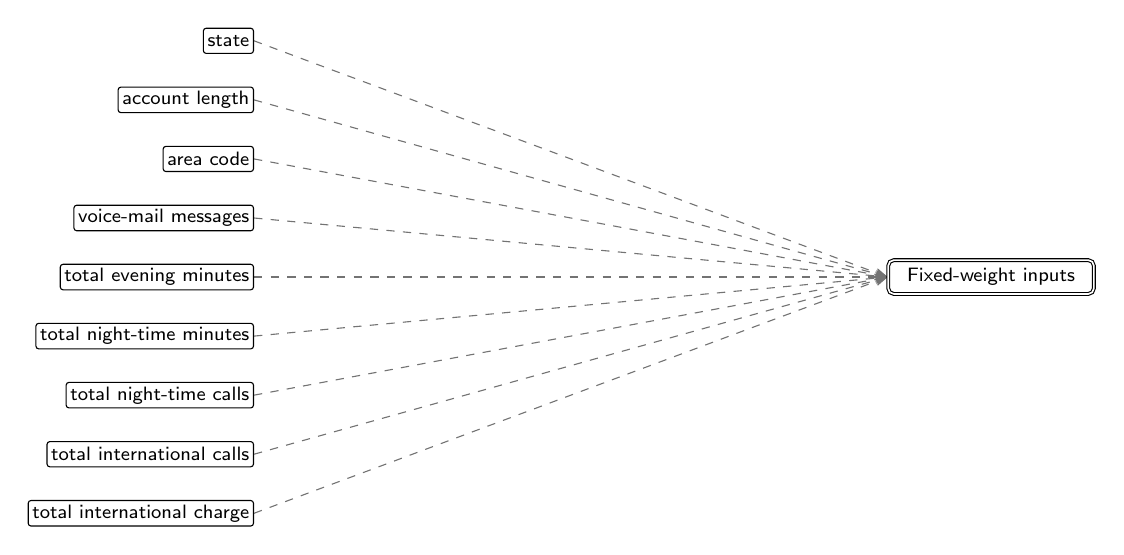
\begin{tikzpicture}[
  font=\sffamily\scriptsize, >={Stealth[length=1.6mm]},
  inp/.style={draw, rounded corners=1pt, fill=white, inner sep=1.5pt, minimum height=3.2mm, anchor=east},
  abox/.style={draw, thick, rounded corners=2pt, align=center, inner sep=3pt, minimum height=6mm, text width=42mm},
  outp/.style={draw, double, rounded corners=2pt, fill=white, align=center, inner sep=3pt, text width=24mm},
  agg/.style={draw=black!55},
]
\node[inp] (i0) at (0,3.0) {state};
\node[inp] (i1) at (0,2.25) {account length};
\node[inp] (i2) at (0,1.5) {area code};
\node[inp] (i3) at (0,0.75) {voice-mail messages};
\node[inp] (i4) at (0,-0.0) {total evening minutes};
\node[inp] (i5) at (0,-0.75) {total night-time minutes};
\node[inp] (i6) at (0,-1.5) {total night-time calls};
\node[inp] (i7) at (0,-2.25) {total international calls};
\node[inp] (i8) at (0,-3.0) {total international charge};
\node[outp] (out) at (9.36,0) {Fixed-weight inputs};
\begin{scope}[on background layer]
\draw[->, agg, thin, dashed] (i0.east) -- (out.west);
\draw[->, agg, thin, dashed] (i1.east) -- (out.west);
\draw[->, agg, thin, dashed] (i2.east) -- (out.west);
\draw[->, agg, thin, dashed] (i3.east) -- (out.west);
\draw[->, agg, thin, dashed] (i4.east) -- (out.west);
\draw[->, agg, thin, dashed] (i5.east) -- (out.west);
\draw[->, agg, thin, dashed] (i6.east) -- (out.west);
\draw[->, agg, thin, dashed] (i7.east) -- (out.west);
\draw[->, agg, thin, dashed] (i8.east) -- (out.west);
\end{scope}
\end{tikzpicture}}}%
\caption{Fixed-weight inputs: what feeds it, one level down.}
\label{fig:churn100s7c1:parts-ann78}
\end{figure}
\begin{figure}[H]\centering
\resizebox{\ifdim\width>\linewidth\linewidth\else\width\fi}{!}{%
\definecolor{netup}{HTML}{D95F02}\definecolor{netdown}{HTML}{1B9E77}\definecolor{netmixed}{HTML}{7F7F7F}%
\begin{tikzpicture}[
  font=\sffamily\scriptsize, >={Stealth[length=1.4mm]},
  inp/.style={draw, circle, fill=white, minimum size=3.2mm, inner sep=0pt},
  hid/.style={draw, circle, fill=white, minimum size=5.2mm, inner sep=0.5pt, font=\sffamily\tiny},
  exitbox/.style={draw, thick, rectangle, fill=white, align=center, text width=17mm, minimum height=5mm, inner sep=1.5pt, font=\sffamily\tiny},
  sumbox/.style={draw, thick, dashed, rectangle, fill=white, align=center, text width=17mm, minimum height=5mm, inner sep=1.5pt, font=\sffamily\tiny},
  outp/.style={draw, thick, regular polygon, regular polygon sides=6, fill=white, minimum size=10mm, inner sep=0pt, font=\sffamily\tiny, align=center},
  stub/.style={draw, dashed, rounded corners=2pt, fill=white, align=center, inner sep=2pt, font=\sffamily\tiny, text width=15mm},
  inlab/.style={font=\sffamily\tiny, align=center, text width=15mm, inner sep=1pt, fill=white, fill opacity=0.8, text opacity=1},
  wpos/.style={draw=NavyBlue}, wneg/.style={draw=BrickRed}, wagg/.style={draw=black!45, line width=1.2pt},
  wmix/.style={draw=Plum},
]
\node[exitbox] (nidentityxlin) at (5.85,1.9) {Fixed-weight inputs $\uparrow$};
\node[inp, draw=netmixed, very thick] (ngrpxxstate) at (2.7,0.0) {};
\path (ngrpxxstate.south) node[inlab, anchor=north] (labngrpxxstate) {state (23 of 51 used) $\updownarrow$};
\node[inp, draw=netup, very thick] (ninxxaccountxlength) at (0.9,0.0) {};
\path (ninxxaccountxlength.south) node[inlab, anchor=north] (labninxxaccountxlength) {account length $\uparrow$};
\node[inp, draw=netup, very thick] (ninxxareaxcodex510) at (1.8,-1.05) {};
\path (ninxxareaxcodex510.south) node[inlab, anchor=north] (labninxxareaxcodex510) {area code 510 $\uparrow$};
\node[inp, draw=netup, very thick] (ninxxnumberxvmailxmessages) at (9.9,0.0) {};
\path (ninxxnumberxvmailxmessages.south) node[inlab, anchor=north] (labninxxnumberxvmailxmessages) {voice-mail messages $\uparrow$};
\node[inp, draw=netup, very thick] (ninxxtotalxnightxcalls) at (6.3,0.0) {};
\path (ninxxtotalxnightxcalls.south) node[inlab, anchor=north] (labninxxtotalxnightxcalls) {total night-time calls $\uparrow$};
\node[inp, draw=netdown, very thick] (ninxxtotalxintlxcalls) at (4.5,0.0) {};
\path (ninxxtotalxintlxcalls.south) node[inlab, anchor=north] (labninxxtotalxintlxcalls) {total international calls $\downarrow$};
\node[inp, draw=netup, very thick] (ninxxtotalxintlxcharge) at (5.4,-1.05) {};
\path (ninxxtotalxintlxcharge.south) node[inlab, anchor=north] (labninxxtotalxintlxcharge) {total international charge $\uparrow$};
\node[inp, draw=netdown, very thick] (ninxxtotalxevexminutes) at (3.6,-1.05) {};
\path (ninxxtotalxevexminutes.south) node[inlab, anchor=north] (labninxxtotalxevexminutes) {total evening minutes $\downarrow$};
\node[inp, draw=netdown, very thick] (ninxxtotalxnightxminutes) at (8.1,0.0) {};
\path (ninxxtotalxnightxminutes.south) node[inlab, anchor=north] (labninxxtotalxnightxminutes) {total night-time minutes $\downarrow$};
\node[stub] (ntoxxthexmodelxoutput) at (5.4,3.45) {to the model output};
\begin{scope}[on background layer]
\node[fit=(nidentityxlin) , inner sep=8pt, rounded corners=5pt, fill=Orchid!10, draw=Orchid!45] (clu0) {};
\draw[->, wpos, line width=0.28pt] (ninxxaccountxlength) -- (nidentityxlin);
\draw[->, wpos, line width=0.27pt] (ninxxareaxcodex510) -- (nidentityxlin);
\draw[->, wpos, line width=0.32pt] (ninxxnumberxvmailxmessages) -- (nidentityxlin);
\draw[->, wpos, line width=0.26pt] (ninxxtotalxnightxcalls) -- (nidentityxlin);
\draw[->, wneg, line width=0.34pt] (ninxxtotalxintlxcalls) -- (nidentityxlin);
\draw[->, wpos, line width=0.36pt] (ninxxtotalxintlxcharge) -- (nidentityxlin);
\draw[->, wneg, line width=0.30pt] (ninxxtotalxevexminutes) -- (nidentityxlin);
\draw[->, wneg, line width=0.29pt] (ninxxtotalxnightxminutes) -- (nidentityxlin);
\draw[->, wpos, line width=0.60pt] (nidentityxlin) -- (ntoxxthexmodelxoutput);
\draw[->, wmix, line width=0.34pt] (ngrpxxstate) -- node[pos=0.8, sloped, above, font=\sffamily\tiny, inner sep=1pt, fill=white, fill opacity=0.8, text opacity=1] {19 edges, -0.26 to +0.15} (nidentityxlin);
\end{scope}
\node[font=\sffamily\scriptsize\bfseries, text=Orchid!55!black, anchor=south west, inner sep=1pt, fill=white, fill opacity=0.85, text opacity=1] at (clu0.north west) {Fixed-weight inputs};
\end{tikzpicture}}%
\caption{Fixed-weight inputs: its units and every connection into them. Blue: positive weight (raises the score); red: negative weight (lowers it); thicker: larger weight. Orange outline and up arrow: raises the final prediction; teal and down arrow: lowers it; grey and double arrow: depends.}
\label{fig:churn100s7c1:units-ann78}
\end{figure}
\paragraph{Hypothesis.} This part adds small fixed-weight effects: a higher international charge, more voice-mail messages and a longer account raise the chance steadily, more international calls lower it, each extra call taking away about the same, and some states shift it up or down.\,{\scriptsize\textcolor{NavyBlue}{[C083, C086, C098, C087, C080, C082]}}
\paragraph{Evidence.} Through it, compared with most other states, Washington raises a typical customer's chance to about 3\% and Montana to about 2\%, and Vermont, Rhode Island and Colorado lower it to under 1\%.\,{\scriptsize\textcolor{NavyBlue}{[C080, C081, C082, C084, C085]}} The international charge raises it steadily, from under 1\% at 1.84 to about 1\% at 3.70 US dollars, and international calls lower it from about 1\% at 2 to under 1\% at 8 calls, each extra call taking away about the same.\,{\scriptsize\textcolor{NavyBlue}{[C083, C087]}} More evening and night-time minutes lower it steadily through this part, by less than a point.\,{\scriptsize\textcolor{NavyBlue}{[C092, C096]}} Its formula reproduces the part exactly on all 4000 training customers.\,{\scriptsize\textcolor{NavyBlue}{[C107]}}
\par\noindent{\small Evidence plots: Figure~\ref{fig:churn100s7c1:plot-ann78-0}, Figure~\ref{fig:churn100s7c1:plot-ann78-1}, Figure~\ref{fig:churn100s7c1:plot-ann78-2}, Figure~\ref{fig:churn100s7c1:plot-ann78-3}.\par}
\begin{figure}[H]\centering
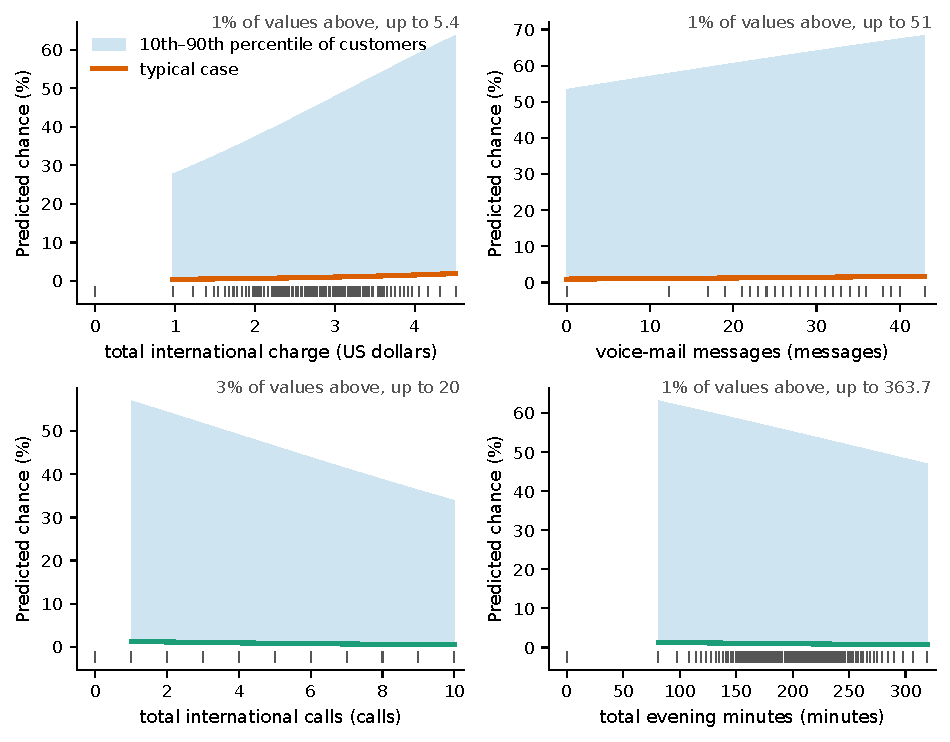
\includegraphics[width=\linewidth,height=0.88\textheight,keepaspectratio]{figures/churn100-s7-c1/ann_78-response.pdf}
\caption{Fixed-weight inputs: Response curves through this part: the typical case (bold), the 10th to 90th percentile of individual customers (band), the fold or step point (dashed) with its spread across them (grey), and the observed values (ticks).}
\label{fig:churn100s7c1:plot-ann78-0}
\end{figure}
\begin{figure}[H]\centering
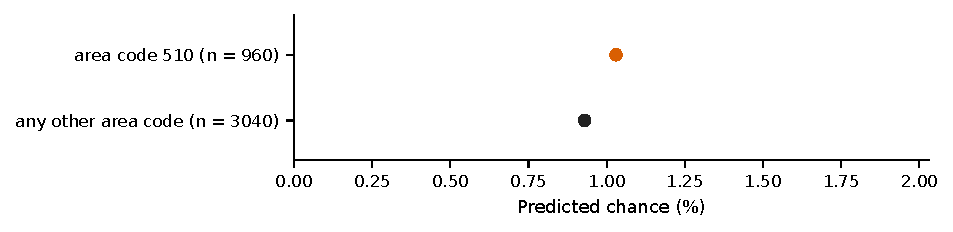
\includegraphics[width=\linewidth,height=0.88\textheight,keepaspectratio]{figures/churn100-s7-c1/ann_78-categories-small.pdf}
\caption{Fixed-weight inputs: The predicted value for the typical case at each level, through this part (n = training customers; grey: fewer than 20).}
\label{fig:churn100s7c1:plot-ann78-1}
\end{figure}
\begin{figure}[H]\centering
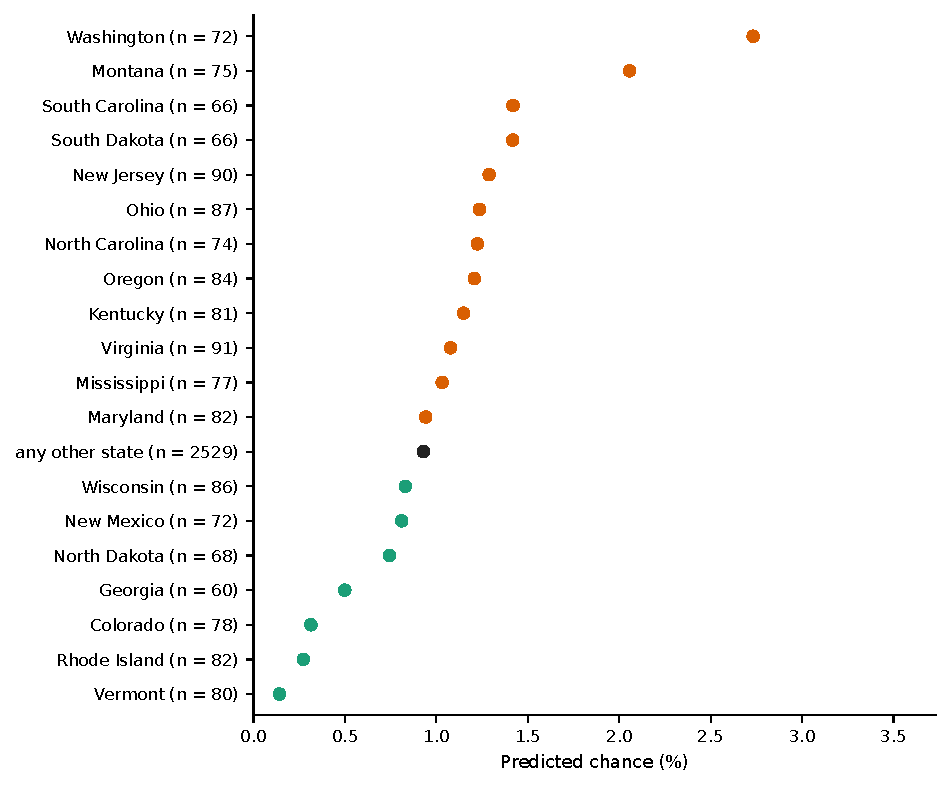
\includegraphics[width=\linewidth,height=0.88\textheight,keepaspectratio]{figures/churn100-s7-c1/ann_78-categories-C080.pdf}
\caption{Fixed-weight inputs: The predicted value for the typical case at each level, through this part (n = training customers; grey: fewer than 20).}
\label{fig:churn100s7c1:plot-ann78-2}
\end{figure}
\begin{figure}[H]\centering
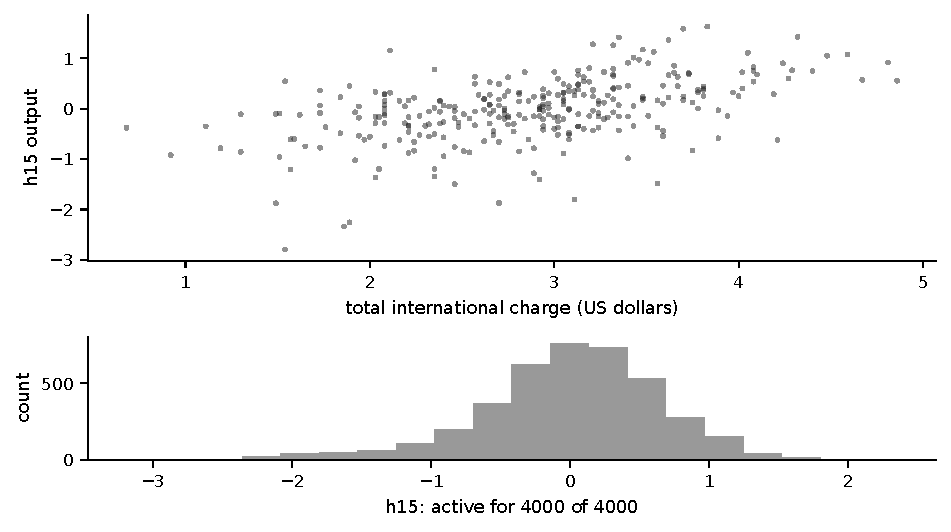
\includegraphics[width=\linewidth,height=0.88\textheight,keepaspectratio]{figures/churn100-s7-c1/ann_78-units.pdf}
\caption{Fixed-weight inputs: This part's hidden units: each unit's output against its main numeric input (top) and how often it is active (bottom).}
\label{fig:churn100s7c1:plot-ann78-3}
\end{figure}
\par\smallskip\noindent{\small Technical detail: \ref{tech:ann78}.\par}
\subsubsection{Voice mail and South Dakota}\label{rd:ann80}
\noindent{\footnotesize Part of: The whole model (\ref{rd:ann84}).\par}
\noindent{\small Figure~\ref{fig:churn100s7c1:parts-ann80} shows what feeds this part; Figure~\ref{fig:churn100s7c1:units-ann80} its units and every connection into them (dashed boxes: connections from or to other parts, drawn in their own sections).\par}
\begin{figure}[H]\centering
\resizebox{!}{\ifdim\height>0.5\textheight 0.5\textheight\else\height\fi}{%
\resizebox{\ifdim\width>\linewidth\linewidth\else\width\fi}{!}{%
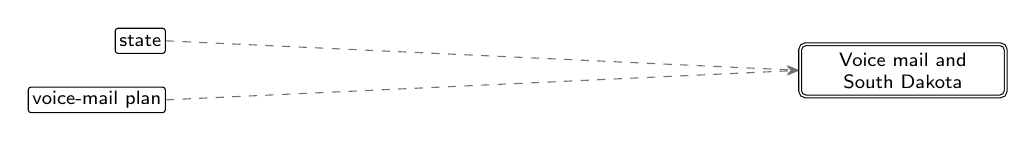
\begin{tikzpicture}[
  font=\sffamily\scriptsize, >={Stealth[length=1.6mm]},
  inp/.style={draw, rounded corners=1pt, fill=white, inner sep=1.5pt, minimum height=3.2mm, anchor=east},
  abox/.style={draw, thick, rounded corners=2pt, align=center, inner sep=3pt, minimum height=6mm, text width=42mm},
  outp/.style={draw, double, rounded corners=2pt, fill=white, align=center, inner sep=3pt, text width=24mm},
  agg/.style={draw=black!55},
]
\node[inp] (i0) at (0,0.375) {state};
\node[inp] (i1) at (0,-0.375) {voice-mail plan};
\node[outp] (out) at (9.36,0) {Voice mail and South Dakota};
\begin{scope}[on background layer]
\draw[->, agg, thin, dashed] (i0.east) -- (out.west);
\draw[->, agg, thin, dashed] (i1.east) -- (out.west);
\end{scope}
\end{tikzpicture}}}%
\caption{Voice mail and South Dakota: what feeds it, one level down.}
\label{fig:churn100s7c1:parts-ann80}
\end{figure}
\begin{figure}[H]\centering
\resizebox{\ifdim\width>\linewidth\linewidth\else\width\fi}{!}{%
\definecolor{netup}{HTML}{D95F02}\definecolor{netdown}{HTML}{1B9E77}\definecolor{netmixed}{HTML}{7F7F7F}%
\begin{tikzpicture}[
  font=\sffamily\scriptsize, >={Stealth[length=1.4mm]},
  inp/.style={draw, circle, fill=white, minimum size=3.2mm, inner sep=0pt},
  hid/.style={draw, circle, fill=white, minimum size=5.2mm, inner sep=0.5pt, font=\sffamily\tiny},
  exitbox/.style={draw, thick, rectangle, fill=white, align=center, text width=17mm, minimum height=5mm, inner sep=1.5pt, font=\sffamily\tiny},
  sumbox/.style={draw, thick, dashed, rectangle, fill=white, align=center, text width=17mm, minimum height=5mm, inner sep=1.5pt, font=\sffamily\tiny},
  outp/.style={draw, thick, regular polygon, regular polygon sides=6, fill=white, minimum size=10mm, inner sep=0pt, font=\sffamily\tiny, align=center},
  stub/.style={draw, dashed, rounded corners=2pt, fill=white, align=center, inner sep=2pt, font=\sffamily\tiny, text width=15mm},
  inlab/.style={font=\sffamily\tiny, align=center, text width=15mm, inner sep=1pt, fill=white, fill opacity=0.8, text opacity=1},
  wpos/.style={draw=NavyBlue}, wneg/.style={draw=BrickRed}, wagg/.style={draw=black!45, line width=1.2pt},
  wmix/.style={draw=Plum},
]
\node[exitbox] (n582) at (2.7,1.9) {Voice mail and South Dakota $\downarrow$};
\node[inp, draw=netmixed, very thick] (ngrpxxstate) at (3.6,0.0) {};
\path (ngrpxxstate.south) node[inlab, anchor=north] (labngrpxxstate) {state (23 of 51 used) $\updownarrow$};
\node[inp, draw=netdown, very thick] (ninxxvoicexmailxplan) at (1.8,0.0) {};
\path (ninxxvoicexmailxplan.south) node[inlab, anchor=north] (labninxxvoicexmailxplan) {a voice-mail plan $\downarrow$};
\node[stub] (ntoxxthexmodelxoutput) at (2.7,3.45) {to the model output};
\begin{scope}[on background layer]
\node[fit=(n582) , inner sep=8pt, rounded corners=5pt, fill=Goldenrod!10, draw=Goldenrod!45] (clu0) {};
\draw[->, wpos, line width=0.31pt] (ninxxvoicexmailxplan) -- (n582);
\draw[->, wneg, line width=0.74pt] (n582) -- (ntoxxthexmodelxoutput);
\draw[->, wpos, line width=0.28pt] (ngrpxxstate) -- node[pos=0.8, sloped, above, font=\sffamily\tiny, inner sep=1pt, fill=white, fill opacity=0.8, text opacity=1] {+0.09} (n582);
\end{scope}
\node[font=\sffamily\scriptsize\bfseries, text=Goldenrod!55!black, anchor=south west, inner sep=1pt, fill=white, fill opacity=0.85, text opacity=1] at (clu0.north west) {Voice mail and South Dakota};
\end{tikzpicture}}%
\caption{Voice mail and South Dakota: its units and every connection into them. Blue: positive weight (raises the score); red: negative weight (lowers it); thicker: larger weight. Orange outline and up arrow: raises the final prediction; teal and down arrow: lowers it; grey and double arrow: depends.}
\label{fig:churn100s7c1:units-ann80}
\end{figure}
\paragraph{Hypothesis.} This part lowers the chance of leaving for customers in South Dakota and for customers with a voice-mail plan.\,{\scriptsize\textcolor{NavyBlue}{[C108, C109]}}
\paragraph{Evidence.} Through it, a customer in South Dakota has under 1\% instead of about 1\%, and a voice-mail plan also takes a typical customer to under 1\%.\,{\scriptsize\textcolor{NavyBlue}{[C108, C109]}} Its formula reproduces the part exactly on all 4000 training customers.\,{\scriptsize\textcolor{NavyBlue}{[C110]}}
\par\noindent{\small Evidence plots: Figure~\ref{fig:churn100s7c1:plot-ann80-0}, Figure~\ref{fig:churn100s7c1:plot-ann80-1}.\par}
\begin{figure}[H]\centering
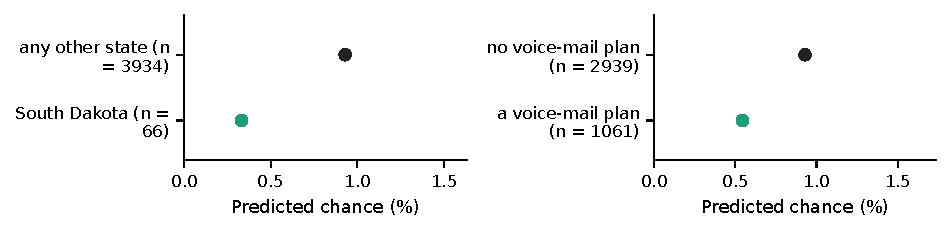
\includegraphics[width=\linewidth,height=0.88\textheight,keepaspectratio]{figures/churn100-s7-c1/ann_80-categories-small.pdf}
\caption{Voice mail and South Dakota: The predicted value for the typical case at each level, through this part (n = training customers; grey: fewer than 20).}
\label{fig:churn100s7c1:plot-ann80-0}
\end{figure}
\begin{figure}[H]\centering
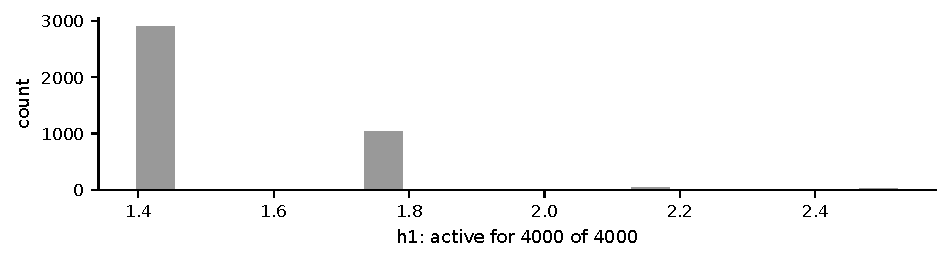
\includegraphics[width=\linewidth,height=0.88\textheight,keepaspectratio]{figures/churn100-s7-c1/ann_80-units.pdf}
\caption{Voice mail and South Dakota: This part's hidden units: each unit's output against its main numeric input (top) and how often it is active (bottom).}
\label{fig:churn100s7c1:plot-ann80-1}
\end{figure}
\par\smallskip\noindent{\small Technical detail: \ref{tech:ann80}.\par}
\subsubsection{State adjustments}\label{rd:ann82}
\noindent{\footnotesize Part of: The whole model (\ref{rd:ann84}).\par}
\noindent{\small Figure~\ref{fig:churn100s7c1:parts-ann82} shows what feeds this part; Figure~\ref{fig:churn100s7c1:units-ann82} its units and every connection into them (dashed boxes: connections from or to other parts, drawn in their own sections).\par}
\begin{figure}[H]\centering
\resizebox{!}{\ifdim\height>0.5\textheight 0.5\textheight\else\height\fi}{%
\resizebox{\ifdim\width>\linewidth\linewidth\else\width\fi}{!}{%
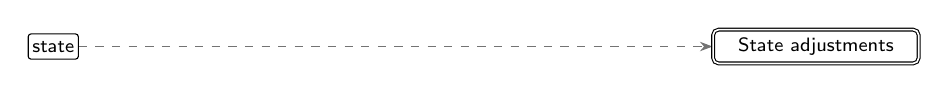
\begin{tikzpicture}[
  font=\sffamily\scriptsize, >={Stealth[length=1.6mm]},
  inp/.style={draw, rounded corners=1pt, fill=white, inner sep=1.5pt, minimum height=3.2mm, anchor=east},
  abox/.style={draw, thick, rounded corners=2pt, align=center, inner sep=3pt, minimum height=6mm, text width=42mm},
  outp/.style={draw, double, rounded corners=2pt, fill=white, align=center, inner sep=3pt, text width=24mm},
  agg/.style={draw=black!55},
]
\node[inp] (i0) at (0,-0.0) {state};
\node[outp] (out) at (9.36,0) {State adjustments};
\begin{scope}[on background layer]
\draw[->, agg, thin, dashed] (i0.east) -- (out.west);
\end{scope}
\end{tikzpicture}}}%
\caption{State adjustments: what feeds it, one level down.}
\label{fig:churn100s7c1:parts-ann82}
\end{figure}
\begin{figure}[H]\centering
\resizebox{\ifdim\width>\linewidth\linewidth\else\width\fi}{!}{%
\definecolor{netup}{HTML}{D95F02}\definecolor{netdown}{HTML}{1B9E77}\definecolor{netmixed}{HTML}{7F7F7F}%
\begin{tikzpicture}[
  font=\sffamily\scriptsize, >={Stealth[length=1.4mm]},
  inp/.style={draw, circle, fill=white, minimum size=3.2mm, inner sep=0pt},
  hid/.style={draw, circle, fill=white, minimum size=5.2mm, inner sep=0.5pt, font=\sffamily\tiny},
  exitbox/.style={draw, thick, rectangle, fill=white, align=center, text width=17mm, minimum height=5mm, inner sep=1.5pt, font=\sffamily\tiny},
  sumbox/.style={draw, thick, dashed, rectangle, fill=white, align=center, text width=17mm, minimum height=5mm, inner sep=1.5pt, font=\sffamily\tiny},
  outp/.style={draw, thick, regular polygon, regular polygon sides=6, fill=white, minimum size=10mm, inner sep=0pt, font=\sffamily\tiny, align=center},
  stub/.style={draw, dashed, rounded corners=2pt, fill=white, align=center, inner sep=2pt, font=\sffamily\tiny, text width=15mm},
  inlab/.style={font=\sffamily\tiny, align=center, text width=15mm, inner sep=1pt, fill=white, fill opacity=0.8, text opacity=1},
  wpos/.style={draw=NavyBlue}, wneg/.style={draw=BrickRed}, wagg/.style={draw=black!45, line width=1.2pt},
  wmix/.style={draw=Plum},
]
\node[hid] (n13420) at (3.35,1.9) {h13};
\node[hid] (n13164) at (1.85,1.9) {h12};
\node[hid] (n12726) at (0.35,1.9) {h11};
\node[hid] (n2067) at (4.85,1.9) {h4};
\node[hid] (n5821) at (7.85,1.9) {h7};
\node[hid] (n5667) at (6.35,1.9) {h6};
\node[inp, draw=netmixed, very thick] (ngrpxxstate) at (4.1,0.0) {};
\path (ngrpxxstate.south) node[inlab, anchor=north] (labngrpxxstate) {state (23 of 51 used) $\updownarrow$};
\node[stub] (ntoxxthexmodelxoutput) at (4.1,3.45) {to the model output};
\begin{scope}[on background layer]
\node[fit=(n13420) (n13164) (n12726) (n2067) (n5821) (n5667) , inner sep=8pt, rounded corners=5pt, fill=Cerulean!10, draw=Cerulean!45] (clu0) {};
\draw[->, wneg, line width=0.34pt] (n2067) -- (ntoxxthexmodelxoutput);
\draw[->, wpos, line width=0.26pt] (n5667) -- (ntoxxthexmodelxoutput);
\draw[->, wneg, line width=0.28pt] (n5821) -- (ntoxxthexmodelxoutput);
\draw[->, wpos, line width=0.26pt] (n12726) -- (ntoxxthexmodelxoutput);
\draw[->, wpos, line width=0.30pt] (n13164) -- (ntoxxthexmodelxoutput);
\draw[->, wneg, line width=0.29pt] (n13420) -- (ntoxxthexmodelxoutput);
\draw[->, wpos, line width=0.61pt] (ngrpxxstate) -- node[pos=0.8, sloped, above, font=\sffamily\tiny, inner sep=1pt, fill=white, fill opacity=0.8, text opacity=1] {+1.02} (n5821);
\draw[->, wneg, line width=0.26pt] (ngrpxxstate) -- node[pos=0.8, sloped, above, font=\sffamily\tiny, inner sep=1pt, fill=white, fill opacity=0.8, text opacity=1] {-0.03} (n5667);
\draw[->, wpos, line width=0.56pt] (ngrpxxstate) -- node[pos=0.8, sloped, above, font=\sffamily\tiny, inner sep=1pt, fill=white, fill opacity=0.8, text opacity=1] {+0.88} (n12726);
\draw[->, wpos, line width=0.60pt] (ngrpxxstate) -- node[pos=0.8, sloped, above, font=\sffamily\tiny, inner sep=1pt, fill=white, fill opacity=0.8, text opacity=1] {+1.01} (n13420);
\draw[->, wpos, line width=0.61pt] (ngrpxxstate) -- node[pos=0.8, sloped, above, font=\sffamily\tiny, inner sep=1pt, fill=white, fill opacity=0.8, text opacity=1] {+1.02} (n13164);
\draw[->, wpos, line width=0.52pt] (ngrpxxstate) -- node[pos=0.8, sloped, above, font=\sffamily\tiny, inner sep=1pt, fill=white, fill opacity=0.8, text opacity=1] {+0.76} (n2067);
\end{scope}
\node[font=\sffamily\scriptsize\bfseries, text=Cerulean!55!black, anchor=south west, inner sep=1pt, fill=white, fill opacity=0.85, text opacity=1] at (clu0.north west) {State adjustments};
\end{tikzpicture}}%
\caption{State adjustments: its units and every connection into them. Blue: positive weight (raises the score); red: negative weight (lowers it); thicker: larger weight. Orange outline and up arrow: raises the final prediction; teal and down arrow: lowers it; grey and double arrow: depends.}
\label{fig:churn100s7c1:units-ann82}
\end{figure}
\paragraph{Hypothesis.} This part shifts the chance of leaving by state: it is lowest in West Virginia and Virginia and highest in South Dakota.\,{\scriptsize\textcolor{NavyBlue}{[C111, C114, C115]}}
\paragraph{Evidence.} Through it, a typical customer's chance is about 5\% in South Dakota and about 2\% in Indiana and in most other states, against about 1\% in West Virginia and under 1\% in Virginia.\,{\scriptsize\textcolor{NavyBlue}{[C111, C112, C114, C115]}} Its formula reproduces the part exactly on all 4000 training customers.\,{\scriptsize\textcolor{NavyBlue}{[C117]}}
\par\noindent{\small Evidence plots: Figure~\ref{fig:churn100s7c1:plot-ann82-0}, Figure~\ref{fig:churn100s7c1:plot-ann82-1}.\par}
\begin{figure}[H]\centering
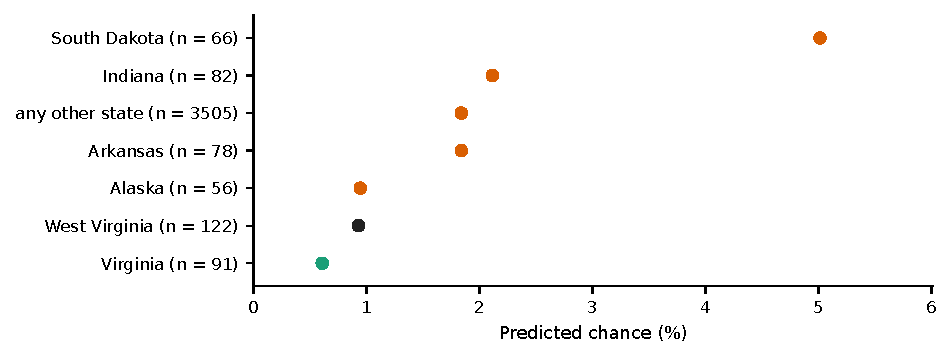
\includegraphics[width=\linewidth,height=0.88\textheight,keepaspectratio]{figures/churn100-s7-c1/ann_82-categories-C111.pdf}
\caption{State adjustments: The predicted value for the typical case at each level, through this part (n = training customers; grey: fewer than 20).}
\label{fig:churn100s7c1:plot-ann82-0}
\end{figure}
\begin{figure}[H]\centering
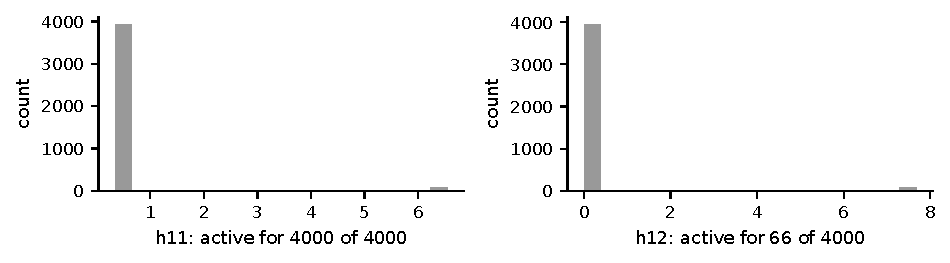
\includegraphics[width=\linewidth,height=0.88\textheight,keepaspectratio]{figures/churn100-s7-c1/ann_82-units.pdf}
\caption{State adjustments: This part's hidden units: each unit's output against its main numeric input (top) and how often it is active (bottom).}
\label{fig:churn100s7c1:plot-ann82-1}
\end{figure}
\par\smallskip\noindent{\small Technical detail: \ref{tech:ann82}.\par}
\subsection{Not supported by the model}
\begin{itemize}\setlength\itemsep{0pt}\small
\item C016: direction claim about total evening minutes in the whole model: not supported by the model (58\% of patients have the opposite sign (allowed: 10\%)).
\item C032: direction claim about total night-time minutes in the whole model: not supported by the model (63\% of patients have the opposite sign (allowed: 10\%)).
\item C058: threshold claim about total night-time minutes in part ann\_\allowbreak{}83: not supported by the model (the folds are spread over 39\% of the observed range (allowed 20\%), also within each category group: no single threshold; the effect past the fold is too small or not consistent across patients).
\item C059: threshold claim about total evening minutes in part ann\_\allowbreak{}83: not supported by the model (the effect past the fold is too small or not consistent across patients; no training patient is past the fold).
\item C069: interaction claim about total daytime minutes and voice-mail plan in part ann\_\allowbreak{}79: not supported by the model (the part's counterfactual difference has the same sign for only 89\% of affected patients).
\item C070: interaction claim about total evening minutes and voice-mail plan in part ann\_\allowbreak{}79: not supported by the model (the part's counterfactual difference has the same sign for only 89\% of affected patients).
\item C073: threshold claim about total night-time minutes in part ann\_\allowbreak{}79: not supported by the model (the folds are spread over 39\% of the observed range (allowed 20\%), also within each category group: no single threshold; the effect past the fold is too small or not consistent across patients).
\item C074: threshold claim about total evening minutes in part ann\_\allowbreak{}79: not supported by the model (the effect past the fold is too small or not consistent across patients; no training patient is past the fold).
\item C075: subgroup claim about state and voice-mail plan in part ann\_\allowbreak{}79: not supported by the model (its effect goes both ways across the patients it acts on).
\item C118: boundary claim about number of calls to customer service and total daytime minutes in part ann\_\allowbreak{}83: not supported by the model (no switch-on line could be traced on the first map to check against the data; no switch-on boundary in the observed range).
\end{itemize}
\clearpage\section*{Technical detail: churn100-s7-c1}
\addcontentsline{toc}{section}{Technical detail: churn100-s7-c1}
\noindent{\small The record behind each part: the original hypothesis, the closed form, and every claim with its estimate (log-odds and odds ratio), range across patients, n and test check.\par}
\renewcommand{\thesubsection}{T.\arabic{subsection}}\setcounter{subsection}{0}
\subsection{The whole model}\label{tech:ann84}
\noindent{\footnotesize Annotation ann\_\allowbreak{}84 (churn\_\allowbreak{}logit). Reads: state, account length, area code, international calling plan, voice-mail plan, number of voice-mail messages, total daytime minutes, total daytime calls, total daytime charge, total evening minutes, total evening calls, total evening charge, total night-time minutes, total night-time calls, total night-time charge, total international minutes, total international calls, total international charge, number of calls to customer service.\par}
\paragraph{Original hypothesis (unchanged).} Root: logit P(churn) = -1.96 + linear\_\allowbreak{}backbone (identity\_\allowbreak{}lin) + usage\_\allowbreak{}response (identity\_\allowbreak{}usage) + 1.68*6711 (intl\_\allowbreak{}plan\_\allowbreak{}switch) - 1.40*582 (vmail\_\allowbreak{}state41\_\allowbreak{}unit) + state\_\allowbreak{}offsets (-0.26*2067 - 0.10*5821 + 0.02*12726 + 0.13*13164 - 0.12*13420 + 0.03*5667), purely additive in the logit; the sigmoid is the only coupling. 35 inputs are unconnected (international minutes, night charge, evening charge and calls, day calls, area codes 408/415 and 29 state indicators) and have zero effect. Train AUC 0.9189, accuracy 0.921. Performance sources (train): all units replaced by least-squares linear fits gives AUC 0.8336 (an L2 logistic regression refit on all 71 inputs gets 0.8433); restoring usage\_\allowbreak{}response alone gives 0.9189 (all the gain); its parts alone: usage hinge 0.8803, heavy-use hinge 0.8870, service-calls gate 0.8731. The international-plan, voicemail and state units are exact switches/offsets and restore nothing. Rare-category switches: state:46 -1.89 logit (80 rows, empirical log-odds offset -0.91); state:39 -1.23 (82, -0.93); state:47 +1.10 (72, +0.92); state:5 -1.09 (78, -0.51); state:45 -0.97 (91, -0.85); state:26 +0.81 (75, +0.50); state:49 -0.69 (122, -0.32); state:0 -0.68 (56, -0.76); state:10 -0.63 (60, -0.22); state:41 +0.25 mean, range -3.85..+0.43 (66, -0.04: it switches off the 1406 day-charge hinge, so heavy users lose up to 3.85).
\paragraph{Closed form.} Read through its parts (their formulas are in their own sections).
\paragraph{Split inputs.} To annotate the parts, the explanation split these inputs into copies (a refactoring step that does not change what the model computes); the diagrams draw each input once: total evening minutes (2 copies); total night-time minutes (2 copies); a voice-mail plan (2 copies).
\paragraph{State: every level the model reads.} Whole-model change in the predicted chance for a typical customer when only the state changes from the reference; n = training customers in that level.\par\smallskip
{\scriptsize\rowcolors{2}{black!6}{white}
\begin{longtable}{@{}lllrlc@{}}
\toprule\rowcolor{white}
Claim & From & To & n & Chance & OK \\
\midrule\endhead
\bottomrule\endfoot
C002 & West Virginia & Washington & 72 & 1\% to 5\% & \textcolor{OliveGreen}{yes} \\
C003 & West Virginia & Montana & 75 & 1\% to 4\% & \textcolor{OliveGreen}{yes} \\
C006 & West Virginia & South Carolina & 66 & 1\% to 3\% & \textcolor{OliveGreen}{yes} \\
C007 & West Virginia & South Dakota & 66 & 1\% to 3\% & \textcolor{OliveGreen}{yes} \\
C008 & West Virginia & New Jersey & 90 & 1\% to 3\% & \textcolor{OliveGreen}{yes} \\
C009 & West Virginia & Ohio & 87 & 1\% to 2\% & \textcolor{OliveGreen}{yes} \\
C010 & West Virginia & North Carolina & 74 & 1\% to 2\% & \textcolor{OliveGreen}{yes} \\
C011 & West Virginia & Oregon & 84 & 1\% to 2\% & \textcolor{OliveGreen}{yes} \\
C012 & West Virginia & Kentucky & 81 & 1\% to 2\% & \textcolor{OliveGreen}{yes} \\
C013 & West Virginia & Indiana & 82 & 1\% to 2\% & \textcolor{OliveGreen}{yes} \\
C014 & West Virginia & Mississippi & 77 & 1\% to 2\% & \textcolor{OliveGreen}{yes} \\
C015 & West Virginia & Maryland & 82 & 1\% to 2\% & \textcolor{OliveGreen}{yes} \\
C017 & West Virginia & Arkansas & 78 & 1\% to 2\% & \textcolor{OliveGreen}{yes} \\
C018 & West Virginia & state other than Alaska, Georgia, Indiana, Kentucky, Arka... & 2191 & 1\% to 2\% & \textcolor{OliveGreen}{yes} \\
C020 & West Virginia & Wisconsin & 86 & 1\% to 2\% & \textcolor{OliveGreen}{yes} \\
C021 & West Virginia & New Mexico & 72 & 1\% to 2\% & \textcolor{OliveGreen}{yes} \\
C024 & West Virginia & North Dakota & 68 & 1\% to 1\% & \textcolor{OliveGreen}{yes} \\
C034 & West Virginia & Georgia & 60 & 1\% to 1\% & \textcolor{OliveGreen}{yes} \\
C036 & West Virginia & Alaska & 56 & 1\% to 1\% & \textcolor{OliveGreen}{yes} \\
C030 & West Virginia & Virginia & 91 & 1\% to 1\% & \textcolor{OliveGreen}{yes} \\
C028 & West Virginia & Colorado & 78 & 1\% to 1\% & \textcolor{OliveGreen}{yes} \\
C026 & West Virginia & Rhode Island & 82 & 1\% to 1\% & \textcolor{OliveGreen}{yes} \\
C022 & West Virginia & Vermont & 80 & 1\% to $<$1\% & \textcolor{OliveGreen}{yes} \\
\end{longtable}}
\paragraph{Evidence table} (next page, landscape).
\begin{landscape}
{\scriptsize\setlength{\tabcolsep}{3pt}\renewcommand{\arraystretch}{1.15}
\rowcolors{2}{black!6}{white}
\begin{longtable}{@{}l>{\raggedright\arraybackslash}p{0.36\linewidth}>{\raggedright\arraybackslash}p{0.14\linewidth}rrr>{\raggedright\arraybackslash}p{0.06\linewidth}>{\raggedright\arraybackslash}p{0.17\linewidth}c@{}}
\toprule\rowcolor{white}
ID & What is checked & Risk, typical patient & Log-odds & OR & Range (p10--p90) & n & Test check & OK \\
\midrule\endfirsthead
\toprule\rowcolor{white}
ID & What is checked & Risk, typical patient & Log-odds & OR & Range (p10--p90) & n & Test check & OK \\
\midrule\endhead
\bottomrule\endfoot
C001 & direction: international calling plan: no international plan to an international plan (whole model) \newline{\itshape shape: categorical; highest to lowest: an international plan, no international plan} & 1\% to 15\% & 2.91 & 18.3 & 2.91 to 2.91 & 3620, 380 & agrees; AUC gain 0.060 [0.033, 0.090] & \textcolor{OliveGreen}{yes} \\
C002 & direction: state: West Virginia to Washington (whole model) \newline{\itshape shape: categorical; highest to lowest: Washington, Montana, South Carolina, South Dakota, New Jersey, Ohio ...} & 1\% to 5\% & 1.79 & 5.98 & 1.79 to 1.79 & 122, 72 & disagrees; AUC gain -0.004 [-0.017, 0.006] & \textcolor{OliveGreen}{yes} \\
C003 & direction: state: West Virginia to Montana (whole model) \newline{\itshape shape: categorical; highest to lowest: Washington, Montana, South Carolina, South Dakota, New Jersey, Ohio ...} & 1\% to 4\% & 1.50 & 4.47 & 1.50 to 1.50 & 122, 75 & disagrees; AUC gain -0.004 [-0.017, 0.006] & \textcolor{OliveGreen}{yes} \\
C004 & direction: total daytime minutes: 112 minutes to 249 minutes (whole model) \newline{\itshape shape: accelerating; 67\% of patients same; fallback; risk saturates near 0\%} & 1\% to 4\% & 1.37 & 3.93 & 0.00 to 4.32 & 4000 & agrees; AUC gain 0.035 [0.016, 0.052] & \textcolor{OliveGreen}{yes} \\
C005 & direction: customer-service calls: 0 calls to 3 calls (whole model) \newline{\itshape shape: accelerating; 89\% of patients same; mixed (but hinge for customers without a voice-mail plan); risk saturates near 0\%} & 1\% to 3\% & 0.86 & 2.37 & 0.00 to 1.25 & 4000 & agrees; AUC gain 0.097 [0.061, 0.136] & \textcolor{OliveGreen}{yes} \\
C006 & direction: state: West Virginia to South Carolina (whole model) \newline{\itshape shape: categorical; highest to lowest: Washington, Montana, South Carolina, South Dakota, New Jersey, Ohio ...} & 1\% to 3\% & 1.12 & 3.06 & 1.12 to 1.12 & 122, 66 & disagrees; AUC gain -0.004 [-0.017, 0.006] & \textcolor{OliveGreen}{yes} \\
C007 & direction: state: West Virginia to South Dakota (whole model) \newline{\itshape shape: categorical; highest to lowest: Washington, Montana, South Carolina, South Dakota, New Jersey, Ohio ...} & 1\% to 3\% & 0.94 & 2.55 & 0.79 to 1.12 & 122, 66 & disagrees; AUC gain -0.004 [-0.017, 0.006] & \textcolor{OliveGreen}{yes} \\
C008 & direction: state: West Virginia to New Jersey (whole model) \newline{\itshape shape: categorical; highest to lowest: Washington, Montana, South Carolina, South Dakota, New Jersey, Ohio ...} & 1\% to 3\% & 1.02 & 2.78 & 1.02 to 1.02 & 122, 90 & disagrees; AUC gain -0.004 [-0.017, 0.006] & \textcolor{OliveGreen}{yes} \\
C009 & direction: state: West Virginia to Ohio (whole model) \newline{\itshape shape: categorical; highest to lowest: Washington, Montana, South Carolina, South Dakota, New Jersey, Ohio ...} & 1\% to 2\% & 0.98 & 2.66 & 0.98 to 0.98 & 122, 87 & disagrees; AUC gain -0.004 [-0.017, 0.006] & \textcolor{OliveGreen}{yes} \\
C010 & direction: state: West Virginia to North Carolina (whole model) \newline{\itshape shape: categorical; highest to lowest: Washington, Montana, South Carolina, South Dakota, New Jersey, Ohio ...} & 1\% to 2\% & 0.97 & 2.64 & 0.97 to 0.97 & 122, 74 & disagrees; AUC gain -0.004 [-0.017, 0.006] & \textcolor{OliveGreen}{yes} \\
C011 & direction: state: West Virginia to Oregon (whole model) \newline{\itshape shape: categorical; highest to lowest: Washington, Montana, South Carolina, South Dakota, New Jersey, Ohio ...} & 1\% to 2\% & 0.96 & 2.60 & 0.96 to 0.96 & 122, 84 & disagrees; AUC gain -0.004 [-0.017, 0.006] & \textcolor{OliveGreen}{yes} \\
C012 & direction: state: West Virginia to Kentucky (whole model) \newline{\itshape shape: categorical; highest to lowest: Washington, Montana, South Carolina, South Dakota, New Jersey, Ohio ...} & 1\% to 2\% & 0.91 & 2.47 & 0.91 to 0.91 & 122, 81 & disagrees; AUC gain -0.004 [-0.017, 0.006] & \textcolor{OliveGreen}{yes} \\
C013 & direction: state: West Virginia to Indiana (whole model) \newline{\itshape shape: categorical; highest to lowest: Washington, Montana, South Carolina, South Dakota, New Jersey, Ohio ...} & 1\% to 2\% & 0.83 & 2.30 & 0.83 to 0.83 & 122, 82 & disagrees; AUC gain -0.004 [-0.017, 0.006] & \textcolor{OliveGreen}{yes} \\
C014 & direction: state: West Virginia to Mississippi (whole model) \newline{\itshape shape: categorical; highest to lowest: Washington, Montana, South Carolina, South Dakota, New Jersey, Ohio ...} & 1\% to 2\% & 0.80 & 2.22 & 0.80 to 0.80 & 122, 77 & disagrees; AUC gain -0.004 [-0.017, 0.006] & \textcolor{OliveGreen}{yes} \\
C015 & direction: state: West Virginia to Maryland (whole model) \newline{\itshape shape: categorical; highest to lowest: Washington, Montana, South Carolina, South Dakota, New Jersey, Ohio ...} & 1\% to 2\% & 0.70 & 2.02 & 0.70 to 0.70 & 122, 82 & disagrees; AUC gain -0.004 [-0.017, 0.006] & \textcolor{OliveGreen}{yes} \\
C016 & direction: total evening minutes: 138 minutes to 266 minutes (whole model) \newline{\itshape shape: dip at 212 minutes; 36\% of patients same; fallback; risk saturates near 0\%} & 1\% to 2\% & 0.67 & 1.96 & -0.35 to 3.65 & 4000 & agrees; AUC gain 0.030 [0.010, 0.050] & \textcolor{BrickRed}{no} \\
C017 & direction: state: West Virginia to Arkansas (whole model) \newline{\itshape shape: categorical; highest to lowest: Washington, Montana, South Carolina, South Dakota, New Jersey, Ohio ...} & 1\% to 2\% & 0.69 & 2.00 & 0.69 to 0.69 & 122, 78 & disagrees; AUC gain -0.004 [-0.017, 0.006] & \textcolor{OliveGreen}{yes} \\
C018 & direction: state: West Virginia to state other than Alaska, Georgia, Indiana, Kentucky, Arkansas, Maryland, Mississippi, Montana, North Carolina, North Dakota, New Jersey, New Mexico, Ohio, Oregon, Rhode Island, South Carolina, South Dakota, Virginia, Vermont, Washington, Wisconsin, West Virginia, Colorado (whole model) \newline{\itshape shape: categorical; highest to lowest: Washington, Montana, South Carolina, South Dakota, New Jersey, Ohio ...} & 1\% to 2\% & 0.69 & 2.00 & 0.69 to 0.69 & 122, 2191 & disagrees; AUC gain -0.004 [-0.017, 0.006] & \textcolor{OliveGreen}{yes} \\
C019 & direction: total international charge: 1.84 US dollars to 3.70 US dollars (whole model) \newline{\itshape shape: steady; 100\% of patients same; verified; risk saturates near 0\%} & 1\% to 1\% & 0.80 & 2.23 & 0.80 to 0.80 & 4000 & unclear; AUC gain 0.003 [-0.005, 0.011] & \textcolor{OliveGreen}{yes} \\
C020 & direction: state: West Virginia to Wisconsin (whole model) \newline{\itshape shape: categorical; highest to lowest: Washington, Montana, South Carolina, South Dakota, New Jersey, Ohio ...} & 1\% to 2\% & 0.58 & 1.78 & 0.58 to 0.58 & 122, 86 & disagrees; AUC gain -0.004 [-0.017, 0.006] & \textcolor{OliveGreen}{yes} \\
C021 & direction: state: West Virginia to New Mexico (whole model) \newline{\itshape shape: categorical; highest to lowest: Washington, Montana, South Carolina, South Dakota, New Jersey, Ohio ...} & 1\% to 2\% & 0.55 & 1.74 & 0.55 to 0.55 & 122, 72 & disagrees; AUC gain -0.004 [-0.017, 0.006] & \textcolor{OliveGreen}{yes} \\
C022 & direction: state: West Virginia to Vermont (whole model) \newline{\itshape shape: categorical; highest to lowest: Washington, Montana, South Carolina, South Dakota, New Jersey, Ohio ...} & 1\% to $<$1\% & -1.20 & 0.30 & -1.20 to -1.20 & 122, 80 & disagrees; AUC gain -0.004 [-0.017, 0.006] & \textcolor{OliveGreen}{yes} \\
C023 & direction: voice-mail messages: 0 messages to 32 messages (whole model) \newline{\itshape shape: steady; 100\% of patients same; verified; risk saturates near 0\%} & 1\% to 1\% & 0.47 & 1.60 & 0.47 to 0.47 & 4000 & unclear; AUC gain 0.0008 [-0.004, 0.006] & \textcolor{OliveGreen}{yes} \\
C024 & direction: state: West Virginia to North Dakota (whole model) \newline{\itshape shape: categorical; highest to lowest: Washington, Montana, South Carolina, South Dakota, New Jersey, Ohio ...} & 1\% to 1\% & 0.47 & 1.60 & 0.47 to 0.47 & 122, 68 & disagrees; AUC gain -0.004 [-0.017, 0.006] & \textcolor{OliveGreen}{yes} \\
C025 & direction: total international calls: 2 calls to 8 calls (whole model) \newline{\itshape shape: steady (equal steps); 100\% of patients same; verified; risk saturates near 0\%} & 1\% to 1\% & -0.63 & 0.53 & -0.63 to -0.63 & 4000 & unclear; AUC gain 0.002 [-0.004, 0.008] & \textcolor{OliveGreen}{yes} \\
C026 & direction: state: West Virginia to Rhode Island (whole model) \newline{\itshape shape: categorical; highest to lowest: Washington, Montana, South Carolina, South Dakota, New Jersey, Ohio ...} & 1\% to 1\% & -0.54 & 0.58 & -0.54 to -0.54 & 122, 82 & disagrees; AUC gain -0.004 [-0.017, 0.006] & \textcolor{OliveGreen}{yes} \\
C027 & direction: voice-mail plan: no voice-mail plan to a voice-mail plan (whole model) \newline{\itshape shape: categorical; highest to lowest: no voice-mail plan, a voice-mail plan} & 1\% to 1\% & -1.37 & 0.25 & -3.46 to -0.54 & 2939, 1061 & agrees; AUC gain 0.019 [0.005, 0.031] & \textcolor{OliveGreen}{yes} \\
C028 & direction: state: West Virginia to Colorado (whole model) \newline{\itshape shape: categorical; highest to lowest: Washington, Montana, South Carolina, South Dakota, New Jersey, Ohio ...} & 1\% to 1\% & -0.40 & 0.67 & -0.40 to -0.40 & 122, 78 & disagrees; AUC gain -0.004 [-0.017, 0.006] & \textcolor{OliveGreen}{yes} \\
C029 & direction: total daytime charge: 19.07 US dollars to 42.40 US dollars (whole model) \newline{\itshape shape: hinge at 40.06 US dollars; 50\% of patients same; fallback; risk saturates near 0\%; matches the fold at 38.81 US dollars} & 1\% to 1\% & 0.24 & 1.27 & 0.00 to 1.11 & 4000 & unclear; AUC gain 0.0003 [-0.007, 0.008] & \textcolor{OliveGreen}{yes} \\
C030 & direction: state: West Virginia to Virginia (whole model) \newline{\itshape shape: categorical; highest to lowest: Washington, Montana, South Carolina, South Dakota, New Jersey, Ohio ...} & 1\% to 1\% & -0.28 & 0.76 & -0.28 to -0.28 & 122, 91 & disagrees; AUC gain -0.004 [-0.017, 0.006] & \textcolor{OliveGreen}{yes} \\
C031 & direction: account length: 48 to 152 (whole model) \newline{\itshape shape: steady; 100\% of patients same; verified; risk saturates near 0\%} & 1\% to 1\% & 0.23 & 1.26 & 0.23 to 0.23 & 4000 & disagrees; AUC gain -0.001 [-0.003, 0.001] & \textcolor{OliveGreen}{yes} \\
C032 & direction: total night-time minutes: 136 minutes to 264 minutes (whole model) \newline{\itshape shape: dip at 218 minutes; 30\% of patients same; fallback; risk saturates near 0\%} & 1\% to 1\% & 0.34 & 1.40 & -0.29 to 2.38 & 4000 & agrees; AUC gain 0.007 [0.0006, 0.013] & \textcolor{BrickRed}{no} \\
C033 & direction: area code: area code other than area code 510 to area code 510 (whole model) \newline{\itshape shape: categorical; highest to lowest: area code 510, area code other than area code 510} & 1\% to 1\% & 0.10 & 1.11 & 0.10 to 0.10 & 3040, 960 & unclear; AUC gain 8e-05 [-0.001, 0.002] & \textcolor{OliveGreen}{yes} \\
C034 & direction: state: West Virginia to Georgia (whole model) \newline{\itshape shape: categorical; highest to lowest: Washington, Montana, South Carolina, South Dakota, New Jersey, Ohio ...} & 1\% to 1\% & 0.07 & 1.07 & 0.07 to 0.07 & 122, 60 & disagrees; AUC gain -0.004 [-0.017, 0.006] & \textcolor{OliveGreen}{yes} \\
C035 & direction: total night-time calls: 74 calls to 125 calls (whole model) \newline{\itshape shape: steady; 100\% of patients same; verified; risk saturates near 0\%} & 1\% to 1\% & 0.06 & 1.07 & 0.06 to 0.06 & 4000 & disagrees; AUC gain -9e-05 [-0.0008, 0.0006] & \textcolor{OliveGreen}{yes} \\
C036 & direction: state: West Virginia to Alaska (whole model) \newline{\itshape shape: categorical; highest to lowest: Washington, Montana, South Carolina, South Dakota, New Jersey, Ohio ...} & 1\% to 1\% & 0.02 & 1.02 & 0.02 to 0.02 & 122, 56 & disagrees; AUC gain -0.004 [-0.017, 0.006] & \textcolor{OliveGreen}{yes} \\
C037 & magnitude: international calling plan: no international plan to an international plan, typical patient \newline{\itshape shape: categorical; highest to lowest: an international plan, no international plan} & 1\% to 15\% & 2.91 & 18.3 &  & 3620, 380 & agrees; AUC gain 0.060 [0.033, 0.090] & \textcolor{OliveGreen}{yes} \\
C038 & magnitude: state: West Virginia to Washington, typical patient \newline{\itshape shape: categorical; highest to lowest: Washington, Montana, South Carolina, South Dakota, New Jersey, Ohio ...} & 1\% to 5\% & 1.79 & 5.98 &  & 122, 72 & disagrees; AUC gain -0.004 [-0.017, 0.006] & \textcolor{OliveGreen}{yes} \\
C039 & magnitude: total daytime minutes: 112 minutes to 249 minutes, typical patient \newline{\itshape shape: accelerating; 67\% of patients same; fallback; risk saturates near 0\%} & 1\% to 4\% & 1.47 & 4.37 &  & 4000 & agrees; AUC gain 0.035 [0.016, 0.052] & \textcolor{OliveGreen}{yes} \\
C040 & magnitude: customer-service calls: 0 calls to 3 calls, typical patient \newline{\itshape shape: accelerating; 89\% of patients same; mixed (but hinge for customers without a voice-mail plan); risk saturates near 0\%} & 1\% to 3\% & 1.25 & 3.50 &  & 4000 & agrees; AUC gain 0.097 [0.061, 0.136] & \textcolor{OliveGreen}{yes} \\
C041 & magnitude: total international charge: 1.84 US dollars to 3.70 US dollars, typical patient \newline{\itshape shape: steady; 100\% of patients same; verified; risk saturates near 0\%} & 1\% to 1\% & 0.80 & 2.23 &  & 4000 & unclear; AUC gain 0.003 [-0.005, 0.011] & \textcolor{OliveGreen}{yes} \\
C042 & null: model ignores total daytime calls (exact rule) &  & 0.00 &  &  & 4000 & train only & \textcolor{OliveGreen}{yes} \\
C043 & null: model ignores total evening calls (exact rule) &  & 0.00 &  &  & 4000 & train only & \textcolor{OliveGreen}{yes} \\
C044 & null: model ignores total evening charge (exact rule) &  & 0.00 &  &  & 4000 & train only & \textcolor{OliveGreen}{yes} \\
C045 & null: model ignores total international minutes (exact rule) &  & 0.00 &  &  & 4000 & train only & \textcolor{OliveGreen}{yes} \\
C046 & null: model ignores total night-time charge (exact rule) &  & 0.00 &  &  & 4000 & train only & \textcolor{OliveGreen}{yes} \\
C047 & structure: made of linear\_\allowbreak{}backbone, usage\_\allowbreak{}response, intl\_\allowbreak{}plan\_\allowbreak{}switch, vmail\_\allowbreak{}state41\_\allowbreak{}unit, state\_\allowbreak{}offsets; added &  &  &  &  & 4000 & train only & \textcolor{OliveGreen}{yes} \\
\end{longtable}}
\end{landscape}
\subsection{Usage and service calls}\label{tech:ann83}
\noindent{\footnotesize Annotation ann\_\allowbreak{}83 (usage\_\allowbreak{}response). Reads: state, voice-mail plan, total daytime minutes, total daytime charge, total evening minutes, total night-time minutes, number of calls to customer service.\par}
\paragraph{Original hypothesis (unchanged).} Composition on usage\_\allowbreak{}hinge: identity\_\allowbreak{}usage = 2.57*879 + 3.06*10552 + 2.88*4344 enters the logit with weight 1. 10552 = relu(-0.64 + 1.17*relu(-0.16 + 1.08*879)) is a second, steeper hinge that opens once 879 exceeds 0.65 (about 240 day minutes at median other use; active for 12\% of customers), so the usage effect accelerates. 4344 = relu(-0.38 + 0.75 calls - 3.24*879) is a service-calls gate: shut for 0-2 calls, open from 3 calls, and closed again by usage (at 3 calls once 879 $>$ 0.14, at 5 calls once 879 $>$ 0.49). Hypothesis: usage and service calls interact non-additively: service calls raise churn only for low-usage customers (or voicemail-plan customers, for whom usage is off), heavy users get the usage hinges instead. Evidence (train): usage logit (879+10552) by day minutes 0.14 ($<$200), 0.58 (200-220), 1.08 (220-240), 2.02 (240-260), 3.43 (260-280), 6.37 ($>$=280); churn 0.10/\allowbreak{}0.06/\allowbreak{}0.14/\allowbreak{}0.26/\allowbreak{}0.46/\allowbreak{}0.67 vs model 0.09/\allowbreak{}0.09/\allowbreak{}0.17/\allowbreak{}0.30/\allowbreak{}0.49/\allowbreak{}0.69. Without a voicemail plan churn reaches 0.84 above 280 minutes (model 0.86), with a plan 0.04 (model 0.09). Gate logit at 0-7 calls: 0/\allowbreak{}0/\allowbreak{}0/\allowbreak{}0.80/\allowbreak{}2.11/\allowbreak{}3.59/\allowbreak{}5.30/\allowbreak{}7.08 (1.25/2.90/4.55/6.20 at 3-6 calls when usage is off, 0.10/0.50/1.05/2.01 when it is on). Churn by calls 0.115/\allowbreak{}0.110/\allowbreak{}0.110/\allowbreak{}0.106/\allowbreak{}0.437/\allowbreak{}0.571/\allowbreak{}0.679/\allowbreak{}0.545 vs model 0.116/\allowbreak{}0.111/\allowbreak{}0.109/\allowbreak{}0.150/\allowbreak{}0.319/\allowbreak{}0.598/\allowbreak{}0.849/\allowbreak{}0.940: the gate opens one call too early (3 calls: +0.80 logit, empirical churn unchanged) and is over-confident from 6 calls (39 customers). Mean ablation of all three terms AUC 0.6557 (the largest drop: full 0.9189); gate alone 0.8202, heavy-use hinge alone 0.9093; linear replacement 0.8336 (R2 0.53/0.29/0.53); restoring usage\_\allowbreak{}response alone onto the all-linear model recovers 0.9189 (all-linear 0.8336), i.e. all of the gain.
\paragraph{Closed form.} Read through its parts (their formulas are in their own sections).
\paragraph{Evidence table} (next page, landscape).
\begin{landscape}
{\scriptsize\setlength{\tabcolsep}{3pt}\renewcommand{\arraystretch}{1.15}
\rowcolors{2}{black!6}{white}
\begin{longtable}{@{}l>{\raggedright\arraybackslash}p{0.36\linewidth}>{\raggedright\arraybackslash}p{0.14\linewidth}rrr>{\raggedright\arraybackslash}p{0.06\linewidth}>{\raggedright\arraybackslash}p{0.17\linewidth}c@{}}
\toprule\rowcolor{white}
ID & What is checked & Risk, typical patient & Log-odds & OR & Range (p10--p90) & n & Test check & OK \\
\midrule\endfirsthead
\toprule\rowcolor{white}
ID & What is checked & Risk, typical patient & Log-odds & OR & Range (p10--p90) & n & Test check & OK \\
\midrule\endhead
\bottomrule\endfoot
C048 & direction: total daytime minutes: 112 minutes to 249 minutes (through this part) \newline{\itshape shape: accelerating; 67\% of patients same; fallback; risk saturates near 0\%} & 1\% to 4\% & 1.37 & 3.93 & 0.00 to 4.32 & 4000 & agrees; AUC gain 0.035 [0.016, 0.052] & \textcolor{OliveGreen}{yes} \\
C049 & direction: customer-service calls: 0 calls to 3 calls (through this part) \newline{\itshape shape: accelerating; 89\% of patients same; mixed (but hinge for customers without a voice-mail plan); risk saturates near 0\%} & 1\% to 3\% & 0.86 & 2.37 & 0.00 to 1.25 & 4000 & agrees; AUC gain 0.097 [0.061, 0.136] & \textcolor{OliveGreen}{yes} \\
C050 & direction: total evening minutes: 138 minutes to 266 minutes (through this part) \newline{\itshape shape: accelerating; 40\% of patients same; fallback; risk saturates near 0\%} & 1\% to 2\% & 1.03 & 2.79 & 0.00 to 4.01 & 4000 & agrees; AUC gain 0.034 [0.013, 0.055] & \textcolor{OliveGreen}{yes} \\
C051 & direction: total night-time minutes: 136 minutes to 264 minutes (through this part) \newline{\itshape shape: hinge at 224 minutes; 35\% of patients same; fallback; risk saturates near 0\%} & 1\% to 1\% & 0.63 & 1.87 & 0.00 to 2.67 & 4000 & agrees; AUC gain 0.01 [0.003, 0.016] & \textcolor{OliveGreen}{yes} \\
C052 & direction: total daytime charge: 19.07 US dollars to 42.40 US dollars (through this part) \newline{\itshape shape: hinge at 38.81 US dollars; 50\% of patients same; fallback; risk saturates near 0\%; one point with C057 (median fold 38.81 US dollars, typical patient 40.06 US dollars, 10th-90th percentile 37.22 US dollars to 53.94 US dollars, wide)} & 1\% to 1\% & 0.24 & 1.27 & 0.00 to 1.11 & 4000 & unclear; AUC gain 0.0003 [-0.007, 0.008] & \textcolor{OliveGreen}{yes} \\
C053 & direction: state: state other than South Dakota to South Dakota (through this part) \newline{\itshape shape: categorical; highest to lowest: South Dakota, state other than South Dakota} & 1\% to 1\% & -0.18 & 0.83 & -0.32 to 0.00 & 3934, 66 & unclear; AUC gain 0.0002 [-0.0002, 0.0007] & \textcolor{OliveGreen}{yes} \\
C054 & direction: voice-mail plan: no voice-mail plan to a voice-mail plan (through this part) \newline{\itshape shape: categorical; highest to lowest: a voice-mail plan, no voice-mail plan} & 1\% to 1\% & -0.83 & 0.44 & -2.92 to 0.00 & 2939, 1061 & agrees; AUC gain 0.013 [0.0009, 0.023] & \textcolor{OliveGreen}{yes} \\
C055 & threshold: customer-service calls: fold at about 3 calls (starts) \newline{\itshape shape: accelerating; 86\% of patients same; mixed (but hinge for customers without a voice-mail plan); risk saturates near 0\%} & 1\% to 15\% (typical patient with a fold) & 2.20 & 9.02 & 0.00 to 2.90 & 3833, 614 & agrees; AUC gain 0.097 [0.061, 0.136] & \textcolor{OliveGreen}{yes} \\
C056 & threshold: total daytime minutes: fold at about 187 minutes (starts) for customers without a voice-mail plan \newline{\itshape shape: accelerating; 67\% of patients same; fallback; risk saturates near 0\%} & 1\% to 11\% (typical patient with a fold) & 2.80 & 16.4 & 0.00 to 6.18 & 3014, 1382 & agrees; AUC gain 0.035 [0.016, 0.052] & \textcolor{OliveGreen}{yes} \\
C057 & threshold: total daytime charge: fold at about 38.81 US dollars (starts) for customers without a voice-mail plan \newline{\itshape shape: hinge at 38.81 US dollars; 45\% of patients same; fallback; risk saturates near 0\%; one point with C057 (median fold 38.81 US dollars, typical patient 36.87 US dollars, 10th-90th percentile 37.22 US dollars to 53.94 US dollars, wide)} & 1\% to 2\% (typical patient with a fold) & 0.73 & 2.07 & 0.00 to 2.28 & 2578, 579 & unclear; AUC gain 0.0003 [-0.007, 0.008] & \textcolor{OliveGreen}{yes} \\
C058 & threshold: total night-time minutes: fold at about 220 minutes (starts) for customers without a voice-mail plan \newline{\itshape shape: hinge at 230 minutes; 45\% of patients same; fallback; risk saturates near 0\%} & 1\% to 2\% (typical patient with a fold) & 0.75 & 2.11 & -0.06 to 2.45 & 2340, 1023 & agrees; AUC gain 0.01 [0.003, 0.016] & \textcolor{BrickRed}{no} \\
C059 & threshold: total evening minutes: fold at about 318 minutes (starts) for customers with a voice-mail plan \newline{\itshape shape: step at 307 minutes; 50\% of patients same; fallback; risk saturates near 0\%} & 2\% to 2\% (typical patient with a fold (customers with a voice-mail plan)) & -0.01 & 0.99 & 0.00 to 0.00 & 43, 0 (small n) & agrees; AUC gain 0.034 [0.013, 0.055] & \textcolor{BrickRed}{no} \\
C060 & structure: made of usage\_\allowbreak{}hinge and inputs number customer service calls; combined non-additively &  &  &  &  & 4000 & train only & \textcolor{OliveGreen}{yes} \\
C118 & boundary: boundary &  &  &  &  & 4000 & train only & \textcolor{BrickRed}{no} \\
\end{longtable}}
\end{landscape}
\subsection{Usage score}\label{tech:ann79}
\noindent{\footnotesize Annotation ann\_\allowbreak{}79 (usage\_\allowbreak{}hinge). Reads: state, voice-mail plan, total daytime minutes, total daytime charge, total evening minutes, total night-time minutes.\par}
\paragraph{Original hypothesis (unchanged).} 879 = relu(-0.99 + 0.53 dayMin + 0.22 nightMin - 1.01 vmailPlan + 0.55*7558), 7558 = relu(0.51 + 0.67 eveMin + 1.21*1406), 1406 = relu(-0.50 + 0.54 dayCharge - 0.88 state:41). Day minutes and day charge are collinear (r = 1.0000), so 879 is a hinge in total usage, dominated by day use. Hypothesis: a usage hinge that is never active for voicemail-plan customers (0 of 1061) and active for 47\% of the rest; at median evening/night use it switches on at about 190 day minutes and rises steadily, with a second slope from the 1406 day-charge hinge (on for 24\% of customers, never in state:41). Its exit feeds the logit directly (weight 2.57) and drives the heavy-use hinge and the service-calls gate in usage\_\allowbreak{}response. Evidence (train, n=4000): sensitivity of 879 to voicemail plan 0.35, day minutes 0.18, evening minutes 0.12, state:41 0.09, night minutes 0.08, day charge 0.05. Mean ablation of its direct logit term AUC 0.9017; linear replacement 0.9107 (R2 0.53); restored alone onto the all-linearised model 0.8803 (all-linear 0.8336).
\paragraph{Closed form} {\footnotesize(weights and biases at 3 significant figures; largest difference from the part on the training patients 8.88178e-16).}
{\small\begingroup\allowdisplaybreaks
\begin{align*}
y_{0} &= \operatorname{relu}\bigl(-0.993 + 0.219 x_{totalNightMinutes\_b} \\
&\qquad + 0.527 x_{totalDayMinutes} + 0.554 \operatorname{relu}\bigl(0.515 \\
&\qquad + 1.21 \operatorname{relu}\bigl(-0.503 + 0.545 x_{totalDayCharge} \\
&\qquad - 0.885 x_{state:41\_c}\bigr) + 0.665 x_{totalEveMinutes\_b}\bigr) \\
&\qquad - 1.01 x_{voiceMailPlan\_b}\bigr)
\end{align*}\endgroup}

\paragraph{Evidence table} (next page, landscape).
\begin{landscape}
{\scriptsize\setlength{\tabcolsep}{3pt}\renewcommand{\arraystretch}{1.15}
\rowcolors{2}{black!6}{white}
\begin{longtable}{@{}l>{\raggedright\arraybackslash}p{0.36\linewidth}>{\raggedright\arraybackslash}p{0.14\linewidth}rrr>{\raggedright\arraybackslash}p{0.06\linewidth}>{\raggedright\arraybackslash}p{0.17\linewidth}c@{}}
\toprule\rowcolor{white}
ID & What is checked & Risk, typical patient & Log-odds & OR & Range (p10--p90) & n & Test check & OK \\
\midrule\endfirsthead
\toprule\rowcolor{white}
ID & What is checked & Risk, typical patient & Log-odds & OR & Range (p10--p90) & n & Test check & OK \\
\midrule\endhead
\bottomrule\endfoot
C061 & direction: total daytime minutes: 112 minutes to 249 minutes (through this part) \newline{\itshape shape: accelerating; 67\% of patients same; fallback; risk saturates near 0\%} & 1\% to 4\% & 1.37 & 3.93 & 0.00 to 4.32 & 4000 & agrees; AUC gain 0.035 [0.016, 0.052] & \textcolor{OliveGreen}{yes} \\
C062 & direction: voice-mail plan: no voice-mail plan to a voice-mail plan (through this part) \newline{\itshape shape: categorical; highest to lowest: no voice-mail plan, a voice-mail plan} & 3\% to 1\% (typical patient this part acts on) & -0.83 & 0.44 & -2.92 to 0.00 & 2939, 1061 & agrees; AUC gain 0.013 [0.0009, 0.023] & \textcolor{OliveGreen}{yes} \\
C063 & direction: total evening minutes: 138 minutes to 266 minutes (through this part) \newline{\itshape shape: accelerating; 40\% of patients same; fallback; risk saturates near 0\%} & 1\% to 2\% & 1.03 & 2.79 & 0.00 to 4.01 & 4000 & agrees; AUC gain 0.034 [0.013, 0.055] & \textcolor{OliveGreen}{yes} \\
C064 & direction: total night-time minutes: 136 minutes to 264 minutes (through this part) \newline{\itshape shape: hinge at 224 minutes; 35\% of patients same; fallback; risk saturates near 0\%} & 1\% to 1\% & 0.63 & 1.87 & 0.00 to 2.67 & 4000 & agrees; AUC gain 0.01 [0.003, 0.016] & \textcolor{OliveGreen}{yes} \\
C065 & direction: total daytime charge: 19.07 US dollars to 42.40 US dollars (through this part) \newline{\itshape shape: hinge at 38.81 US dollars; 50\% of patients same; fallback; risk saturates near 0\%; one point with C072 (median fold 38.81 US dollars, typical patient 40.06 US dollars, 10th-90th percentile 37.22 US dollars to 53.94 US dollars, wide)} & 1\% to 1\% & 0.24 & 1.27 & 0.00 to 1.11 & 4000 & unclear; AUC gain 0.0003 [-0.007, 0.008] & \textcolor{OliveGreen}{yes} \\
C066 & direction: state: state other than South Dakota to South Dakota (through this part) \newline{\itshape shape: categorical; highest to lowest: South Dakota, state other than South Dakota} & 3\% to 3\% (typical patient this part acts on) & -0.18 & 0.83 & -0.32 to 0.00 & 3934, 66 & unclear; AUC gain 0.0002 [-0.0002, 0.0007] & \textcolor{OliveGreen}{yes} \\
C067 & interaction: effect of total daytime minutes (112 minutes to 249 minutes) by total evening minutes: total evening minutes above 201 minutes minus total evening minutes at or below 201 minutes; stronger in total evening minutes above 201 minutes \newline{\itshape shape: accelerating; 75\% of patients same; fallback; risk saturates near 0\%} & total evening minutes above 201 minutes: 1\% to 11\%; total evening minutes at or below 201 minutes: 1\% to 2\% & 1.54 & 4.66 &  & 1998, 2002 & agrees; AUC gain 0.034 [0.013, 0.055] & \textcolor{OliveGreen}{yes} \\
C068 & interaction: effect of total daytime minutes (112 minutes to 249 minutes) by total night-time minutes: total night-time minutes above 200 minutes minus total night-time minutes at or below 200 minutes; stronger in total night-time minutes above 200 minutes \newline{\itshape shape: accelerating; 74\% of patients same; fallback; risk saturates near 0\%} & total night-time minutes above 200 minutes: 1\% to 7\%; total night-time minutes at or below 200 minutes: 1\% to 3\% & 1.00 & 2.71 &  & 2000, 2000 & agrees; AUC gain 0.01 [0.003, 0.016] & \textcolor{OliveGreen}{yes} \\
C069 & interaction: effect of total daytime minutes (112 minutes to 249 minutes) by voice-mail plan: a voice-mail plan minus no voice-mail plan; stronger in no voice-mail plan \newline{\itshape shape: accelerating; 70\% of patients same; fallback; risk saturates near 0\%} & a voice-mail plan: 1\% to 1\%; no voice-mail plan: 1\% to 4\% & -1.86 & 0.16 &  & 1061, 2939 & agrees; AUC gain 0.013 [0.0009, 0.023] & \textcolor{BrickRed}{no} \\
C070 & interaction: effect of total evening minutes (138 minutes to 266 minutes) by voice-mail plan: a voice-mail plan minus no voice-mail plan; stronger in no voice-mail plan \newline{\itshape shape: dip at 212 minutes; 48\% of patients same; fallback; risk saturates near 0\%} & a voice-mail plan: 1\% to $<$1\%; no voice-mail plan: 1\% to 2\% & -1.40 & 0.25 &  & 1061, 2939 & agrees; AUC gain 0.013 [0.0009, 0.023] & \textcolor{BrickRed}{no} \\
C071 & threshold: total daytime minutes: fold at about 187 minutes (starts) for customers without a voice-mail plan \newline{\itshape shape: accelerating; 67\% of patients same; fallback; risk saturates near 0\%} & 1\% to 11\% (typical patient with a fold) & 2.80 & 16.4 & 0.00 to 6.18 & 3014, 1382 & agrees; AUC gain 0.035 [0.016, 0.052] & \textcolor{OliveGreen}{yes} \\
C072 & threshold: total daytime charge: fold at about 38.81 US dollars (starts) for customers without a voice-mail plan \newline{\itshape shape: hinge at 38.81 US dollars; 45\% of patients same; fallback; risk saturates near 0\%; one point with C072 (median fold 38.81 US dollars, typical patient 36.87 US dollars, 10th-90th percentile 37.22 US dollars to 53.94 US dollars, wide)} & 1\% to 2\% (typical patient with a fold) & 0.73 & 2.07 & 0.00 to 2.28 & 2578, 579 & unclear; AUC gain 0.0003 [-0.007, 0.008] & \textcolor{OliveGreen}{yes} \\
C073 & threshold: total night-time minutes: fold at about 220 minutes (starts) for customers without a voice-mail plan \newline{\itshape shape: hinge at 230 minutes; 45\% of patients same; fallback; risk saturates near 0\%} & 1\% to 2\% (typical patient with a fold) & 0.75 & 2.11 & -0.06 to 2.45 & 2340, 1023 & agrees; AUC gain 0.01 [0.003, 0.016] & \textcolor{BrickRed}{no} \\
C074 & threshold: total evening minutes: fold at about 318 minutes (starts) for customers with a voice-mail plan \newline{\itshape shape: step at 307 minutes; 50\% of patients same; fallback; risk saturates near 0\%} & 2\% to 2\% (typical patient with a fold (customers with a voice-mail plan)) & -0.01 & 0.99 & 0.00 to 0.00 & 43, 0 (small n) & agrees; AUC gain 0.034 [0.013, 0.055] & \textcolor{BrickRed}{no} \\
C075 & subgroup: who this part acts on: 1382 of 4000 patients & 1\% to 3\% (typical patient this part acts on (risk without the part, then with it)) & 1.77 & 5.86 & -0.34 to 5.50 & 1382, 2618 & agrees; AUC gain 0.214 [0.160, 0.273] & \textcolor{BrickRed}{no} \\
C076 & structure: its formula reproduces it on 4000 training patients (largest difference 8.88178e-16) &  & 9e-16 &  &  & 4000 & train only & \textcolor{OliveGreen}{yes} \\
C119 & boundary: boundary &  & 1.00 &  &  & 4000 & train only & \textcolor{OliveGreen}{yes} \\
\end{longtable}}
\end{landscape}
\subsection{International plan}\label{tech:ann81}
\noindent{\footnotesize Annotation ann\_\allowbreak{}81 (intl\_\allowbreak{}plan\_\allowbreak{}switch). Reads: international calling plan.\par}
\paragraph{Original hypothesis (unchanged).} 6711 = relu(-0.23 + 0.64 intlPlan), logit weight +1.68: exactly 0 for customers without an international plan and +2.91 logit for the 380 with one (R2 1.0). Hypothesis: an international-plan switch, the model's only route for the plan (no direct edge). Empirical churn 0.42 with the plan vs 0.11 without; model 0.45 vs 0.11. No interaction with international usage (international minutes are unconnected; international charge and calls act linearly in the backbone). Evidence: line plot correlation 1.00; mean ablation AUC 0.8611; linear replacement 0.9189 (identical, exact switch).
\paragraph{Closed form} {\footnotesize(weights and biases at 3 significant figures; largest difference from the part on the training patients 0.0).}
{\small\begingroup\allowdisplaybreaks
\begin{align*}
y_{0} &= \operatorname{relu}\bigl(-0.228 + 0.635 x_{internationalPlan}\bigr)
\end{align*}\endgroup}

\paragraph{Evidence table} (next page, landscape).
\begin{landscape}
{\scriptsize\setlength{\tabcolsep}{3pt}\renewcommand{\arraystretch}{1.15}
\rowcolors{2}{black!6}{white}
\begin{longtable}{@{}l>{\raggedright\arraybackslash}p{0.36\linewidth}>{\raggedright\arraybackslash}p{0.14\linewidth}rrr>{\raggedright\arraybackslash}p{0.06\linewidth}>{\raggedright\arraybackslash}p{0.17\linewidth}c@{}}
\toprule\rowcolor{white}
ID & What is checked & Risk, typical patient & Log-odds & OR & Range (p10--p90) & n & Test check & OK \\
\midrule\endfirsthead
\toprule\rowcolor{white}
ID & What is checked & Risk, typical patient & Log-odds & OR & Range (p10--p90) & n & Test check & OK \\
\midrule\endhead
\bottomrule\endfoot
C077 & direction: international calling plan: no international plan to an international plan (through this part) \newline{\itshape shape: categorical; highest to lowest: an international plan, no international plan} & 1\% to 15\% & 2.91 & 18.3 & 2.91 to 2.91 & 3620, 380 & agrees; AUC gain 0.060 [0.033, 0.090] & \textcolor{OliveGreen}{yes} \\
C078 & subgroup: who this part acts on: 380 of 4000 patients & 2\% to 26\% (typical patient this part acts on (risk without the part, then with it)) & 2.91 & 18.3 & 2.91 to 2.91 & 380, 3620 & agrees; AUC gain 0.060 [0.033, 0.090] & \textcolor{OliveGreen}{yes} \\
C079 & structure: its formula reproduces it on 4000 training patients (largest difference 0.0) &  & 0.00 &  &  & 4000 & train only & \textcolor{OliveGreen}{yes} \\
\end{longtable}}
\end{landscape}
\subsection{Fixed-weight inputs}\label{tech:ann78}
\noindent{\footnotesize Annotation ann\_\allowbreak{}78 (linear\_\allowbreak{}backbone). Reads: state, account length, area code, number of voice-mail messages, total evening minutes, total night-time minutes, total night-time calls, total international calls, total international charge.\par}
\paragraph{Original hypothesis (unchanged).} Direct input-to-output edges collected through identity\_\allowbreak{}lin (an identity node). Exactly linear in 27 inputs, all with small weights (at most 0.32 per SD): international charge +0.32, international calls -0.26, voicemail messages +0.20, evening minutes -0.14 and night minutes -0.11 (these two also feed the usage hinge with positive weights), account length +0.09, area code 510 +0.04 (+0.10 logit), and state offsets: state:46 -1.89 logit (80 customers), state:39 -1.23 (82), state:47 +1.10 (72), state:5 -1.09 (78), state:26 +0.81, state:10 -0.63, state:40 +0.43, state:41 +0.43, state:31 +0.33, then smaller. International plan, voicemail plan, day minutes and customer-service calls have NO direct edge. Evidence: closed form exact (identity, R2 1.0); train sensitivities equal the weights (international charge 0.32, international calls 0.26, state:46 0.26, voicemail messages 0.20). Mean ablation AUC 0.9076 (full 0.9189).
\paragraph{Closed form} {\footnotesize(weights and biases at 3 significant figures; largest difference from the part on the training patients 6.66134e-16).}
{\small\begingroup\allowdisplaybreaks
\begin{align*}
y_{0} &= 0.321 x_{totalIntlCharge} + 0.199 x_{numberVmailMessages} + 0.042 x_{state:35} \\
&\qquad + 0.0442 x_{areaCode:510} + 0.0249 x_{totalNightCalls} + 0.0544 x_{state:41\_a} \\
&\qquad + 0.0545 x_{state:40} + 0.0145 x_{state:25} + 0.00187 x_{state:20} + 0.0301 x_{state:17} \\
&\qquad + 0.146 x_{state:47} + 0.0375 x_{state:27} + 0.0379 x_{state:37} + 0.0871 x_{accountLength} \\
&\qquad + 0.0223 x_{state:45\_a} + 0.049 x_{state:31} + 0.109 x_{state:26} - 0.0289 x_{state:28} \\
&\qquad - 0.139 x_{totalEveMinutes\_a} - 0.175 x_{state:39} - 0.264 x_{totalIntlCalls} \\
&\qquad - 0.0184 x_{state:32} - 0.0761 x_{state:10} - 0.114 x_{totalNightMinutes\_a} \\
&\qquad - 0.0165 x_{state:48} - 0.264 x_{state:46} - 0.151 x_{state:5}
\end{align*}\endgroup}

\paragraph{Evidence table} (next page, landscape).
\begin{landscape}
{\scriptsize\setlength{\tabcolsep}{3pt}\renewcommand{\arraystretch}{1.15}
\rowcolors{2}{black!6}{white}
\begin{longtable}{@{}l>{\raggedright\arraybackslash}p{0.36\linewidth}>{\raggedright\arraybackslash}p{0.14\linewidth}rrr>{\raggedright\arraybackslash}p{0.06\linewidth}>{\raggedright\arraybackslash}p{0.17\linewidth}c@{}}
\toprule\rowcolor{white}
ID & What is checked & Risk, typical patient & Log-odds & OR & Range (p10--p90) & n & Test check & OK \\
\midrule\endfirsthead
\toprule\rowcolor{white}
ID & What is checked & Risk, typical patient & Log-odds & OR & Range (p10--p90) & n & Test check & OK \\
\midrule\endhead
\bottomrule\endfoot
C080 & direction: state: state other than Georgia, Kentucky, Maryland, Mississippi, Montana, North Carolina, North Dakota, New Jersey, New Mexico, Ohio, Oregon, Rhode Island, South Carolina, South Dakota, Virginia, Vermont, Washington, Wisconsin, Colorado to Washington (through this part) \newline{\itshape shape: categorical; highest to lowest: Washington, Montana, South Carolina, South Dakota, New Jersey, Ohio ...} & 1\% to 3\% & 1.10 & 2.99 & 1.10 to 1.10 & 2529, 72 & disagrees; AUC gain -0.004 [-0.016, 0.006] & \textcolor{OliveGreen}{yes} \\
C081 & direction: state: state other than Georgia, Kentucky, Maryland, Mississippi, Montana, North Carolina, North Dakota, New Jersey, New Mexico, Ohio, Oregon, Rhode Island, South Carolina, South Dakota, Virginia, Vermont, Washington, Wisconsin, Colorado to Montana (through this part) \newline{\itshape shape: categorical; highest to lowest: Washington, Montana, South Carolina, South Dakota, New Jersey, Ohio ...} & 1\% to 2\% & 0.81 & 2.24 & 0.81 to 0.81 & 2529, 75 & disagrees; AUC gain -0.004 [-0.016, 0.006] & \textcolor{OliveGreen}{yes} \\
C082 & direction: state: state other than Georgia, Kentucky, Maryland, Mississippi, Montana, North Carolina, North Dakota, New Jersey, New Mexico, Ohio, Oregon, Rhode Island, South Carolina, South Dakota, Virginia, Vermont, Washington, Wisconsin, Colorado to Vermont (through this part) \newline{\itshape shape: categorical; highest to lowest: Washington, Montana, South Carolina, South Dakota, New Jersey, Ohio ...} & 1\% to $<$1\% & -1.89 & 0.15 & -1.89 to -1.89 & 2529, 80 & disagrees; AUC gain -0.004 [-0.016, 0.006] & \textcolor{OliveGreen}{yes} \\
C083 & direction: total international charge: 1.84 US dollars to 3.70 US dollars (through this part) \newline{\itshape shape: steady; 100\% of patients same; verified; risk saturates near 0\%} & 1\% to 1\% & 0.80 & 2.23 & 0.80 to 0.80 & 4000 & unclear; AUC gain 0.003 [-0.005, 0.011] & \textcolor{OliveGreen}{yes} \\
C084 & direction: state: state other than Georgia, Kentucky, Maryland, Mississippi, Montana, North Carolina, North Dakota, New Jersey, New Mexico, Ohio, Oregon, Rhode Island, South Carolina, South Dakota, Virginia, Vermont, Washington, Wisconsin, Colorado to Rhode Island (through this part) \newline{\itshape shape: categorical; highest to lowest: Washington, Montana, South Carolina, South Dakota, New Jersey, Ohio ...} & 1\% to $<$1\% & -1.23 & 0.29 & -1.23 to -1.23 & 2529, 82 & disagrees; AUC gain -0.004 [-0.016, 0.006] & \textcolor{OliveGreen}{yes} \\
C085 & direction: state: state other than Georgia, Kentucky, Maryland, Mississippi, Montana, North Carolina, North Dakota, New Jersey, New Mexico, Ohio, Oregon, Rhode Island, South Carolina, South Dakota, Virginia, Vermont, Washington, Wisconsin, Colorado to Colorado (through this part) \newline{\itshape shape: categorical; highest to lowest: Washington, Montana, South Carolina, South Dakota, New Jersey, Ohio ...} & 1\% to $<$1\% & -1.09 & 0.34 & -1.09 to -1.09 & 2529, 78 & disagrees; AUC gain -0.004 [-0.016, 0.006] & \textcolor{OliveGreen}{yes} \\
C086 & direction: voice-mail messages: 0 messages to 32 messages (through this part) \newline{\itshape shape: steady; 100\% of patients same; verified; risk saturates near 0\%} & 1\% to 1\% & 0.47 & 1.60 & 0.47 to 0.47 & 4000 & unclear; AUC gain 0.0008 [-0.004, 0.006] & \textcolor{OliveGreen}{yes} \\
C087 & direction: total international calls: 2 calls to 8 calls (through this part) \newline{\itshape shape: steady (equal steps); 100\% of patients same; verified; risk saturates near 0\%} & 1\% to 1\% & -0.63 & 0.53 & -0.63 to -0.63 & 4000 & unclear; AUC gain 0.002 [-0.004, 0.008] & \textcolor{OliveGreen}{yes} \\
C088 & direction: state: state other than Georgia, Kentucky, Maryland, Mississippi, Montana, North Carolina, North Dakota, New Jersey, New Mexico, Ohio, Oregon, Rhode Island, South Carolina, South Dakota, Virginia, Vermont, Washington, Wisconsin, Colorado to South Carolina (through this part) \newline{\itshape shape: categorical; highest to lowest: Washington, Montana, South Carolina, South Dakota, New Jersey, Ohio ...} & 1\% to 1\% & 0.43 & 1.53 & 0.43 to 0.43 & 2529, 66 & disagrees; AUC gain -0.004 [-0.016, 0.006] & \textcolor{OliveGreen}{yes} \\
C089 & direction: state: state other than Georgia, Kentucky, Maryland, Mississippi, Montana, North Carolina, North Dakota, New Jersey, New Mexico, Ohio, Oregon, Rhode Island, South Carolina, South Dakota, Virginia, Vermont, Washington, Wisconsin, Colorado to South Dakota (through this part) \newline{\itshape shape: categorical; highest to lowest: Washington, Montana, South Carolina, South Dakota, New Jersey, Ohio ...} & 1\% to 1\% & 0.43 & 1.53 & 0.43 to 0.43 & 2529, 66 & disagrees; AUC gain -0.004 [-0.016, 0.006] & \textcolor{OliveGreen}{yes} \\
C090 & direction: state: state other than Georgia, Kentucky, Maryland, Mississippi, Montana, North Carolina, North Dakota, New Jersey, New Mexico, Ohio, Oregon, Rhode Island, South Carolina, South Dakota, Virginia, Vermont, Washington, Wisconsin, Colorado to Georgia (through this part) \newline{\itshape shape: categorical; highest to lowest: Washington, Montana, South Carolina, South Dakota, New Jersey, Ohio ...} & 1\% to $<$1\% & -0.63 & 0.53 & -0.63 to -0.63 & 2529, 60 & disagrees; AUC gain -0.004 [-0.016, 0.006] & \textcolor{OliveGreen}{yes} \\
C091 & direction: state: state other than Georgia, Kentucky, Maryland, Mississippi, Montana, North Carolina, North Dakota, New Jersey, New Mexico, Ohio, Oregon, Rhode Island, South Carolina, South Dakota, Virginia, Vermont, Washington, Wisconsin, Colorado to New Jersey (through this part) \newline{\itshape shape: categorical; highest to lowest: Washington, Montana, South Carolina, South Dakota, New Jersey, Ohio ...} & 1\% to 1\% & 0.33 & 1.39 & 0.33 to 0.33 & 2529, 90 & disagrees; AUC gain -0.004 [-0.016, 0.006] & \textcolor{OliveGreen}{yes} \\
C092 & direction: total evening minutes: 138 minutes to 266 minutes (through this part) \newline{\itshape shape: steady; 100\% of patients same; verified; risk saturates near 0\%} & 1\% to 1\% & -0.35 & 0.70 & -0.35 to -0.35 & 4000 & disagrees; AUC gain -0.002 [-0.005, 0.0005] & \textcolor{OliveGreen}{yes} \\
C093 & direction: state: state other than Georgia, Kentucky, Maryland, Mississippi, Montana, North Carolina, North Dakota, New Jersey, New Mexico, Ohio, Oregon, Rhode Island, South Carolina, South Dakota, Virginia, Vermont, Washington, Wisconsin, Colorado to Ohio (through this part) \newline{\itshape shape: categorical; highest to lowest: Washington, Montana, South Carolina, South Dakota, New Jersey, Ohio ...} & 1\% to 1\% & 0.29 & 1.33 & 0.29 to 0.29 & 2529, 87 & disagrees; AUC gain -0.004 [-0.016, 0.006] & \textcolor{OliveGreen}{yes} \\
C094 & direction: state: state other than Georgia, Kentucky, Maryland, Mississippi, Montana, North Carolina, North Dakota, New Jersey, New Mexico, Ohio, Oregon, Rhode Island, South Carolina, South Dakota, Virginia, Vermont, Washington, Wisconsin, Colorado to North Carolina (through this part) \newline{\itshape shape: categorical; highest to lowest: Washington, Montana, South Carolina, South Dakota, New Jersey, Ohio ...} & 1\% to 1\% & 0.28 & 1.32 & 0.28 to 0.28 & 2529, 74 & disagrees; AUC gain -0.004 [-0.016, 0.006] & \textcolor{OliveGreen}{yes} \\
C095 & direction: state: state other than Georgia, Kentucky, Maryland, Mississippi, Montana, North Carolina, North Dakota, New Jersey, New Mexico, Ohio, Oregon, Rhode Island, South Carolina, South Dakota, Virginia, Vermont, Washington, Wisconsin, Colorado to Oregon (through this part) \newline{\itshape shape: categorical; highest to lowest: Washington, Montana, South Carolina, South Dakota, New Jersey, Ohio ...} & 1\% to 1\% & 0.26 & 1.30 & 0.26 to 0.26 & 2529, 84 & disagrees; AUC gain -0.004 [-0.016, 0.006] & \textcolor{OliveGreen}{yes} \\
C096 & direction: total night-time minutes: 136 minutes to 264 minutes (through this part) \newline{\itshape shape: steady; 100\% of patients same; verified; risk saturates near 0\%} & 1\% to 1\% & -0.29 & 0.75 & -0.29 to -0.29 & 4000 & disagrees; AUC gain -0.002 [-0.006, 0.0006] & \textcolor{OliveGreen}{yes} \\
C097 & direction: state: state other than Georgia, Kentucky, Maryland, Mississippi, Montana, North Carolina, North Dakota, New Jersey, New Mexico, Ohio, Oregon, Rhode Island, South Carolina, South Dakota, Virginia, Vermont, Washington, Wisconsin, Colorado to Kentucky (through this part) \newline{\itshape shape: categorical; highest to lowest: Washington, Montana, South Carolina, South Dakota, New Jersey, Ohio ...} & 1\% to 1\% & 0.21 & 1.24 & 0.21 to 0.21 & 2529, 81 & disagrees; AUC gain -0.004 [-0.016, 0.006] & \textcolor{OliveGreen}{yes} \\
C098 & direction: account length: 48 to 152 (through this part) \newline{\itshape shape: steady; 100\% of patients same; verified; risk saturates near 0\%} & 1\% to 1\% & 0.23 & 1.26 & 0.23 to 0.23 & 4000 & disagrees; AUC gain -0.001 [-0.003, 0.001] & \textcolor{OliveGreen}{yes} \\
C099 & direction: state: state other than Georgia, Kentucky, Maryland, Mississippi, Montana, North Carolina, North Dakota, New Jersey, New Mexico, Ohio, Oregon, Rhode Island, South Carolina, South Dakota, Virginia, Vermont, Washington, Wisconsin, Colorado to North Dakota (through this part) \newline{\itshape shape: categorical; highest to lowest: Washington, Montana, South Carolina, South Dakota, New Jersey, Ohio ...} & 1\% to 1\% & -0.22 & 0.80 & -0.22 to -0.22 & 2529, 68 & disagrees; AUC gain -0.004 [-0.016, 0.006] & \textcolor{OliveGreen}{yes} \\
C100 & direction: state: state other than Georgia, Kentucky, Maryland, Mississippi, Montana, North Carolina, North Dakota, New Jersey, New Mexico, Ohio, Oregon, Rhode Island, South Carolina, South Dakota, Virginia, Vermont, Washington, Wisconsin, Colorado to Virginia (through this part) \newline{\itshape shape: categorical; highest to lowest: Washington, Montana, South Carolina, South Dakota, New Jersey, Ohio ...} & 1\% to 1\% & 0.15 & 1.16 & 0.15 to 0.15 & 2529, 91 & disagrees; AUC gain -0.004 [-0.016, 0.006] & \textcolor{OliveGreen}{yes} \\
C101 & direction: state: state other than Georgia, Kentucky, Maryland, Mississippi, Montana, North Carolina, North Dakota, New Jersey, New Mexico, Ohio, Oregon, Rhode Island, South Carolina, South Dakota, Virginia, Vermont, Washington, Wisconsin, Colorado to New Mexico (through this part) \newline{\itshape shape: categorical; highest to lowest: Washington, Montana, South Carolina, South Dakota, New Jersey, Ohio ...} & 1\% to 1\% & -0.14 & 0.87 & -0.14 to -0.14 & 2529, 72 & disagrees; AUC gain -0.004 [-0.016, 0.006] & \textcolor{OliveGreen}{yes} \\
C102 & direction: state: state other than Georgia, Kentucky, Maryland, Mississippi, Montana, North Carolina, North Dakota, New Jersey, New Mexico, Ohio, Oregon, Rhode Island, South Carolina, South Dakota, Virginia, Vermont, Washington, Wisconsin, Colorado to Mississippi (through this part) \newline{\itshape shape: categorical; highest to lowest: Washington, Montana, South Carolina, South Dakota, New Jersey, Ohio ...} & 1\% to 1\% & 0.11 & 1.11 & 0.11 to 0.11 & 2529, 77 & disagrees; AUC gain -0.004 [-0.016, 0.006] & \textcolor{OliveGreen}{yes} \\
C103 & direction: area code: area code other than area code 510 to area code 510 (through this part) \newline{\itshape shape: categorical; highest to lowest: area code 510, area code other than area code 510} & 1\% to 1\% & 0.10 & 1.11 & 0.10 to 0.10 & 3040, 960 & unclear; AUC gain 8e-05 [-0.001, 0.002] & \textcolor{OliveGreen}{yes} \\
C104 & direction: state: state other than Georgia, Kentucky, Maryland, Mississippi, Montana, North Carolina, North Dakota, New Jersey, New Mexico, Ohio, Oregon, Rhode Island, South Carolina, South Dakota, Virginia, Vermont, Washington, Wisconsin, Colorado to Wisconsin (through this part) \newline{\itshape shape: categorical; highest to lowest: Washington, Montana, South Carolina, South Dakota, New Jersey, Ohio ...} & 1\% to 1\% & -0.11 & 0.89 & -0.11 to -0.11 & 2529, 86 & disagrees; AUC gain -0.004 [-0.016, 0.006] & \textcolor{OliveGreen}{yes} \\
C105 & direction: total night-time calls: 74 calls to 125 calls (through this part) \newline{\itshape shape: steady; 100\% of patients same; verified; risk saturates near 0\%} & 1\% to 1\% & 0.06 & 1.07 & 0.06 to 0.06 & 4000 & disagrees; AUC gain -9e-05 [-0.0008, 0.0006] & \textcolor{OliveGreen}{yes} \\
C106 & direction: state: state other than Georgia, Kentucky, Maryland, Mississippi, Montana, North Carolina, North Dakota, New Jersey, New Mexico, Ohio, Oregon, Rhode Island, South Carolina, South Dakota, Virginia, Vermont, Washington, Wisconsin, Colorado to Maryland (through this part) \newline{\itshape shape: categorical; highest to lowest: Washington, Montana, South Carolina, South Dakota, New Jersey, Ohio ...} & 1\% to 1\% & 0.01 & 1.01 & 0.01 to 0.01 & 2529, 82 & disagrees; AUC gain -0.004 [-0.016, 0.006] & \textcolor{OliveGreen}{yes} \\
C107 & structure: its formula reproduces it on 4000 training patients (largest difference 6.66134e-16) &  & 7e-16 &  &  & 4000 & train only & \textcolor{OliveGreen}{yes} \\
\end{longtable}}
\end{landscape}
\subsection{Voice mail and South Dakota}\label{tech:ann80}
\noindent{\footnotesize Annotation ann\_\allowbreak{}80 (vmail\_\allowbreak{}state41\_\allowbreak{}unit). Reads: state, voice-mail plan.\par}
\paragraph{Original hypothesis (unchanged).} 582 = relu(1.51 + 0.17 vmailPlan + 0.09 state:41), logit weight -1.40. The pre-activation stays between 1.40 and 2.52 on train, so the unit is always active and exactly affine (R2 1.0): a constant -1.96 logit for customers without a voicemail plan outside state:41, -0.54 extra for a voicemail plan and -1.04 extra for state:41. Hypothesis: a fixed offset plus a voicemail-plan and state:41 discount. Evidence: sensitivity 0.17 (voicemail plan), 0.09 (state:41); linear replacement AUC 0.9189 (unchanged), mean ablation 0.9184.
\paragraph{Closed form} {\footnotesize(weights and biases at 3 significant figures; largest difference from the part on the training patients 4.44089e-16).}
{\small\begingroup\allowdisplaybreaks
\begin{align*}
y_{0} &= \operatorname{relu}\bigl(1.51 + 0.17 x_{voiceMailPlan\_a} \\
&\qquad + 0.0942 x_{state:41\_b}\bigr)
\end{align*}\endgroup}

\paragraph{Evidence table} (next page, landscape).
\begin{landscape}
{\scriptsize\setlength{\tabcolsep}{3pt}\renewcommand{\arraystretch}{1.15}
\rowcolors{2}{black!6}{white}
\begin{longtable}{@{}l>{\raggedright\arraybackslash}p{0.36\linewidth}>{\raggedright\arraybackslash}p{0.14\linewidth}rrr>{\raggedright\arraybackslash}p{0.06\linewidth}>{\raggedright\arraybackslash}p{0.17\linewidth}c@{}}
\toprule\rowcolor{white}
ID & What is checked & Risk, typical patient & Log-odds & OR & Range (p10--p90) & n & Test check & OK \\
\midrule\endfirsthead
\toprule\rowcolor{white}
ID & What is checked & Risk, typical patient & Log-odds & OR & Range (p10--p90) & n & Test check & OK \\
\midrule\endhead
\bottomrule\endfoot
C108 & direction: state: state other than South Dakota to South Dakota (through this part) \newline{\itshape shape: categorical; highest to lowest: state other than South Dakota, South Dakota} & 1\% to $<$1\% & -1.04 & 0.35 & -1.04 to -1.04 & 3934, 66 & agrees; AUC gain 0.001 [0.0004, 0.002] & \textcolor{OliveGreen}{yes} \\
C109 & direction: voice-mail plan: no voice-mail plan to a voice-mail plan (through this part) \newline{\itshape shape: categorical; highest to lowest: no voice-mail plan, a voice-mail plan} & 1\% to 1\% & -0.54 & 0.58 & -0.54 to -0.54 & 2939, 1061 & unclear; AUC gain 0.002 [-0.003, 0.008] & \textcolor{OliveGreen}{yes} \\
C110 & structure: its formula reproduces it on 4000 training patients (largest difference 4.44089e-16) &  & 4e-16 &  &  & 4000 & train only & \textcolor{OliveGreen}{yes} \\
\end{longtable}}
\end{landscape}
\subsection{State adjustments}\label{tech:ann82}
\noindent{\footnotesize Annotation ann\_\allowbreak{}82 (state\_\allowbreak{}offsets). Reads: state.\par}
\paragraph{Original hypothesis (unchanged).} Six single-state units, each a function of one binary indicator and so exactly an offset (R2 1.0): 2067 state:45 -1.12 logit (91 customers; with its direct +0.15, net -0.97), 13164 state:41 +1.04 (66; it offsets most of state:41's -1.04 in vmail\_\allowbreak{}state41\_\allowbreak{}unit), 13420 state:49 -0.69 (122), 5821 state:0 -0.68 (56), 12726 state:15 +0.14 (82; always active, constant +0.008), 5667 state:2 is never active (dead unit, zero effect). Hypothesis: per-state offsets. Evidence: sensitivities as listed; linear replacement AUC 0.9189 (unchanged); mean ablation 0.9167.
\paragraph{Closed form} {\footnotesize(weights and biases at 3 significant figures; largest difference from the part on the training patients 0.0).}
{\small\begingroup\allowdisplaybreaks
\begin{align*}
y_{0} &= \operatorname{relu}\bigl(-0.691 + 0.757 x_{state:45\_b}\bigr) \\
y_{1} &= \operatorname{relu}\bigl(-1.7 + 1.02 x_{state:0}\bigr) \\
y_{2} &= \operatorname{relu}\bigl(0.47 + 0.878 x_{state:15}\bigr) \\
y_{3} &= \operatorname{relu}\bigl(-0.236 + 1.02 x_{state:41\_d}\bigr) \\
y_{4} &= \operatorname{relu}\bigl(0.00575 + 1.01 x_{state:49}\bigr) \\
y_{5} &= \operatorname{relu}\bigl(-0.325 - 0.0317 x_{state:2}\bigr)
\end{align*}\endgroup}

\paragraph{Evidence table} (next page, landscape).
\begin{landscape}
{\scriptsize\setlength{\tabcolsep}{3pt}\renewcommand{\arraystretch}{1.15}
\rowcolors{2}{black!6}{white}
\begin{longtable}{@{}l>{\raggedright\arraybackslash}p{0.36\linewidth}>{\raggedright\arraybackslash}p{0.14\linewidth}rrr>{\raggedright\arraybackslash}p{0.06\linewidth}>{\raggedright\arraybackslash}p{0.17\linewidth}c@{}}
\toprule\rowcolor{white}
ID & What is checked & Risk, typical patient & Log-odds & OR & Range (p10--p90) & n & Test check & OK \\
\midrule\endfirsthead
\toprule\rowcolor{white}
ID & What is checked & Risk, typical patient & Log-odds & OR & Range (p10--p90) & n & Test check & OK \\
\midrule\endhead
\bottomrule\endfoot
C111 & direction: state: West Virginia to South Dakota (through this part) \newline{\itshape shape: categorical; highest to lowest: South Dakota, Indiana, Arkansas, state other than Alaska, Indiana, Arkansas, South Dakota, Virginia, West Virginia, Alaska, West Virginia ...} & 1\% to 5\% & 1.73 & 5.62 & 1.73 to 1.73 & 122, 66 & disagrees; AUC gain -0.0004 [-0.006, 0.004] & \textcolor{OliveGreen}{yes} \\
C112 & direction: state: West Virginia to Indiana (through this part) \newline{\itshape shape: categorical; highest to lowest: South Dakota, Indiana, Arkansas, state other than Alaska, Indiana, Arkansas, South Dakota, Virginia, West Virginia, Alaska, West Virginia ...} & 1\% to 2\% & 0.83 & 2.30 & 0.83 to 0.83 & 122, 82 & disagrees; AUC gain -0.0004 [-0.006, 0.004] & \textcolor{OliveGreen}{yes} \\
C113 & direction: state: West Virginia to Arkansas (through this part) \newline{\itshape shape: categorical; highest to lowest: South Dakota, Indiana, Arkansas, state other than Alaska, Indiana, Arkansas, South Dakota, Virginia, West Virginia, Alaska, West Virginia ...} & 1\% to 2\% & 0.69 & 2.00 & 0.69 to 0.69 & 122, 78 & disagrees; AUC gain -0.0004 [-0.006, 0.004] & \textcolor{OliveGreen}{yes} \\
C114 & direction: state: West Virginia to state other than Alaska, Indiana, Arkansas, South Dakota, Virginia, West Virginia (through this part) \newline{\itshape shape: categorical; highest to lowest: South Dakota, Indiana, Arkansas, state other than Alaska, Indiana, Arkansas, South Dakota, Virginia, West Virginia, Alaska, West Virginia ...} & 1\% to 2\% & 0.69 & 2.00 & 0.69 to 0.69 & 122, 3505 & disagrees; AUC gain -0.0004 [-0.006, 0.004] & \textcolor{OliveGreen}{yes} \\
C115 & direction: state: West Virginia to Virginia (through this part) \newline{\itshape shape: categorical; highest to lowest: South Dakota, Indiana, Arkansas, state other than Alaska, Indiana, Arkansas, South Dakota, Virginia, West Virginia, Alaska, West Virginia ...} & 1\% to 1\% & -0.43 & 0.65 & -0.43 to -0.43 & 122, 91 & disagrees; AUC gain -0.0004 [-0.006, 0.004] & \textcolor{OliveGreen}{yes} \\
C116 & direction: state: West Virginia to Alaska (through this part) \newline{\itshape shape: categorical; highest to lowest: South Dakota, Indiana, Arkansas, state other than Alaska, Indiana, Arkansas, South Dakota, Virginia, West Virginia, Alaska, West Virginia ...} & 1\% to 1\% & 0.02 & 1.02 & 0.02 to 0.02 & 122, 56 & disagrees; AUC gain -0.0004 [-0.006, 0.004] & \textcolor{OliveGreen}{yes} \\
C117 & structure: its formula reproduces it on 4000 training patients (largest difference 0.0) &  & 0.00 &  &  & 4000 & train only & \textcolor{OliveGreen}{yes} \\
\end{longtable}}
\end{landscape}
\subsection*{The network before any explanation}\addcontentsline{toc}{subsection}{The network before any explanation} Figure~\ref{fig:churn100s7c1:raw} (next page, landscape) is the trained network as it is, with no parts, no splits and no inserted units: inputs at the bottom, hidden units by depth, the output at the top, every connection drawn, every input column its own node (one-hot levels included).
\begin{landscape}
\begin{figure}[p]\centering
\resizebox{\linewidth}{!}{%
\definecolor{netup}{HTML}{D95F02}\definecolor{netdown}{HTML}{1B9E77}\definecolor{netmixed}{HTML}{7F7F7F}%
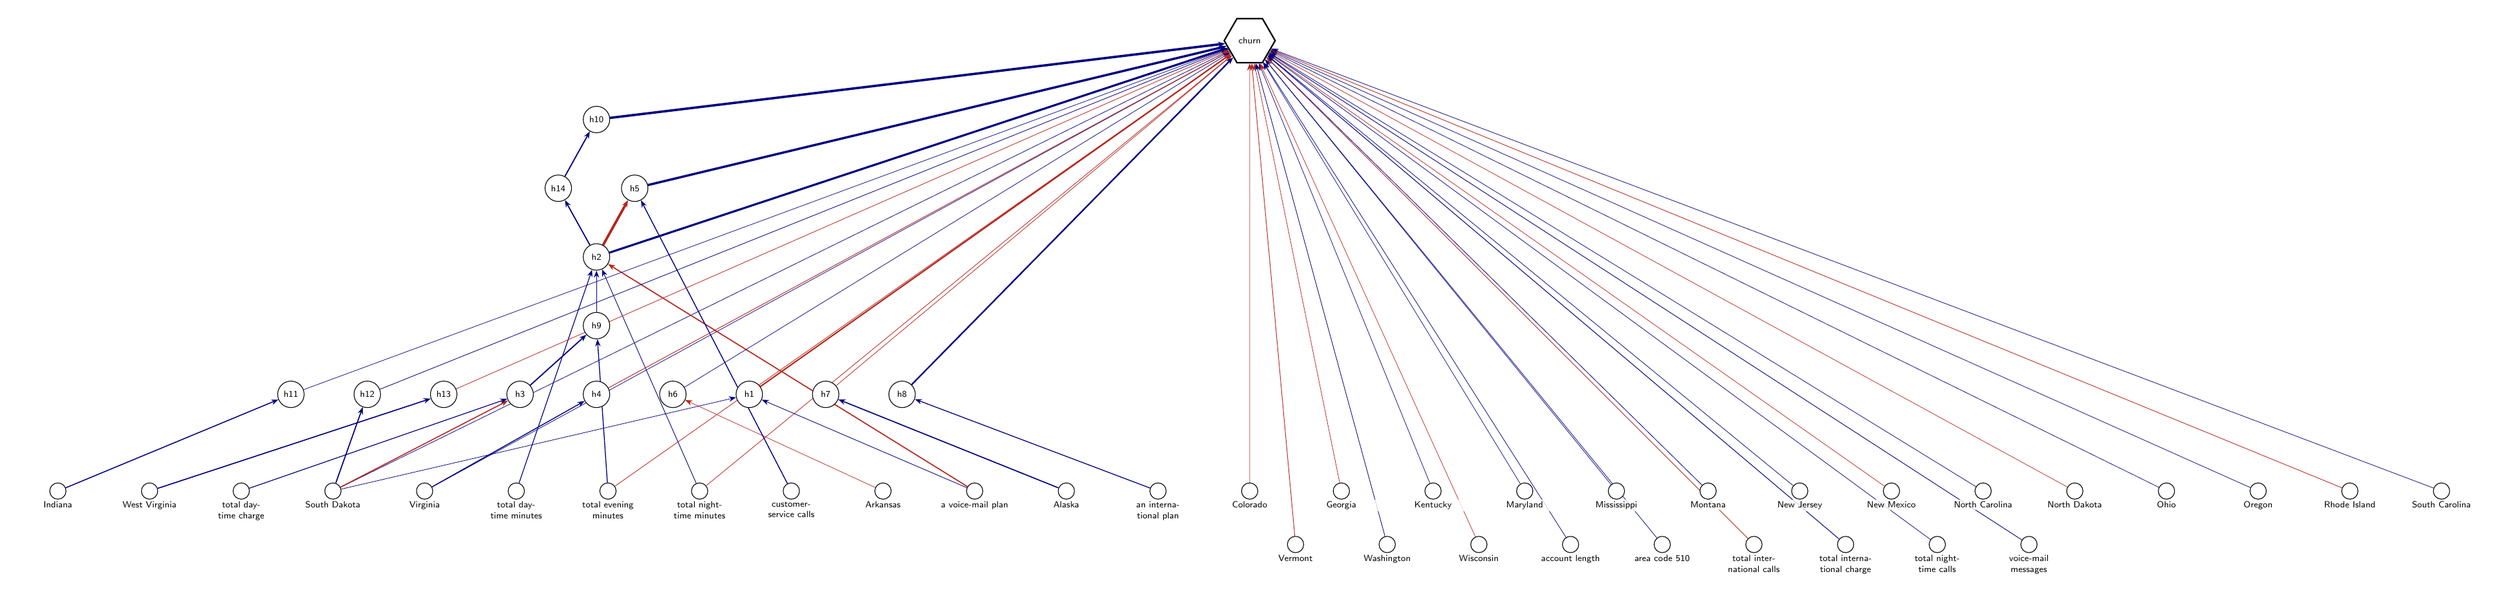
\begin{tikzpicture}[
  font=\sffamily\scriptsize, >={Stealth[length=1.4mm]},
  inp/.style={draw, circle, fill=white, minimum size=3.2mm, inner sep=0pt},
  hid/.style={draw, circle, fill=white, minimum size=5.2mm, inner sep=0.5pt, font=\sffamily\tiny},
  exitbox/.style={draw, thick, rectangle, fill=white, align=center, text width=17mm, minimum height=5mm, inner sep=1.5pt, font=\sffamily\tiny},
  sumbox/.style={draw, thick, dashed, rectangle, fill=white, align=center, text width=17mm, minimum height=5mm, inner sep=1.5pt, font=\sffamily\tiny},
  outp/.style={draw, thick, regular polygon, regular polygon sides=6, fill=white, minimum size=10mm, inner sep=0pt, font=\sffamily\tiny, align=center},
  stub/.style={draw, dashed, rounded corners=2pt, fill=white, align=center, inner sep=2pt, font=\sffamily\tiny, text width=15mm},
  inlab/.style={font=\sffamily\tiny, align=center, text width=15mm, inner sep=1pt, fill=white, fill opacity=0.8, text opacity=1},
  wpos/.style={draw=NavyBlue}, wneg/.style={draw=BrickRed}, wagg/.style={draw=black!45, line width=1.2pt},
  wmix/.style={draw=Plum},
]
\node[inp] (ninxxstatex0) at (19.8,0.0) {};
\path (ninxxstatex0.south) node[inlab, anchor=north] (labninxxstatex0) {Alaska};
\node[inp] (ninxxstatex17) at (27.0,0.0) {};
\path (ninxxstatex17.south) node[inlab, anchor=north] (labninxxstatex17) {Kentucky};
\node[inp] (ninxxstatex2) at (16.2,0.0) {};
\path (ninxxstatex2.south) node[inlab, anchor=north] (labninxxstatex2) {Arkansas};
\node[inp] (ninxxstatex20) at (28.8,0.0) {};
\path (ninxxstatex20.south) node[inlab, anchor=north] (labninxxstatex20) {Maryland};
\node[inp] (ninxxstatex25) at (30.6,0.0) {};
\path (ninxxstatex25.south) node[inlab, anchor=north] (labninxxstatex25) {Mississippi};
\node[inp] (ninxxstatex26) at (32.4,0.0) {};
\path (ninxxstatex26.south) node[inlab, anchor=north] (labninxxstatex26) {Montana};
\node[inp] (ninxxstatex27) at (37.8,0.0) {};
\path (ninxxstatex27.south) node[inlab, anchor=north] (labninxxstatex27) {North Carolina};
\node[inp] (ninxxstatex28) at (39.6,0.0) {};
\path (ninxxstatex28.south) node[inlab, anchor=north] (labninxxstatex28) {North Dakota};
\node[inp] (ninxxstatex31) at (34.2,0.0) {};
\path (ninxxstatex31.south) node[inlab, anchor=north] (labninxxstatex31) {New Jersey};
\node[inp] (ninxxstatex32) at (36.0,0.0) {};
\path (ninxxstatex32.south) node[inlab, anchor=north] (labninxxstatex32) {New Mexico};
\node[inp] (ninxxstatex10) at (25.2,0.0) {};
\path (ninxxstatex10.south) node[inlab, anchor=north] (labninxxstatex10) {Georgia};
\node[inp] (ninxxstatex35) at (41.4,0.0) {};
\path (ninxxstatex35.south) node[inlab, anchor=north] (labninxxstatex35) {Ohio};
\node[inp] (ninxxstatex37) at (43.2,0.0) {};
\path (ninxxstatex37.south) node[inlab, anchor=north] (labninxxstatex37) {Oregon};
\node[inp] (ninxxstatex39) at (45.0,0.0) {};
\path (ninxxstatex39.south) node[inlab, anchor=north] (labninxxstatex39) {Rhode Island};
\node[inp] (ninxxstatex40) at (46.8,0.0) {};
\path (ninxxstatex40.south) node[inlab, anchor=north] (labninxxstatex40) {South Carolina};
\node[inp] (ninxxstatex41) at (5.4,0.0) {};
\path (ninxxstatex41.south) node[inlab, anchor=north] (labninxxstatex41) {South Dakota};
\node[inp] (ninxxstatex45) at (7.2,0.0) {};
\path (ninxxstatex45.south) node[inlab, anchor=north] (labninxxstatex45) {Virginia};
\node[inp] (ninxxstatex46) at (24.3,-1.05) {};
\path (ninxxstatex46.south) node[inlab, anchor=north] (labninxxstatex46) {Vermont};
\node[inp] (ninxxstatex47) at (26.1,-1.05) {};
\path (ninxxstatex47.south) node[inlab, anchor=north] (labninxxstatex47) {Washington};
\node[inp] (ninxxstatex48) at (27.9,-1.05) {};
\path (ninxxstatex48.south) node[inlab, anchor=north] (labninxxstatex48) {Wisconsin};
\node[inp] (ninxxstatex49) at (1.8,0.0) {};
\path (ninxxstatex49.south) node[inlab, anchor=north] (labninxxstatex49) {West Virginia};
\node[inp] (ninxxstatex5) at (23.4,0.0) {};
\path (ninxxstatex5.south) node[inlab, anchor=north] (labninxxstatex5) {Colorado};
\node[inp] (ninxxaccountxlength) at (29.7,-1.05) {};
\path (ninxxaccountxlength.south) node[inlab, anchor=north] (labninxxaccountxlength) {account length};
\node[inp] (ninxxareaxcodex510) at (31.5,-1.05) {};
\path (ninxxareaxcodex510.south) node[inlab, anchor=north] (labninxxareaxcodex510) {area code 510};
\node[inp] (ninxxinternationalxplan) at (21.6,0.0) {};
\path (ninxxinternationalxplan.south) node[inlab, anchor=north] (labninxxinternationalxplan) {an international plan};
\node[inp] (ninxxvoicexmailxplan) at (18.0,0.0) {};
\path (ninxxvoicexmailxplan.south) node[inlab, anchor=north] (labninxxvoicexmailxplan) {a voice-mail plan};
\node[inp] (ninxxnumberxvmailxmessages) at (38.7,-1.05) {};
\path (ninxxnumberxvmailxmessages.south) node[inlab, anchor=north] (labninxxnumberxvmailxmessages) {voice-mail messages};
\node[inp] (ninxxtotalxdayxminutes) at (9.0,0.0) {};
\path (ninxxtotalxdayxminutes.south) node[inlab, anchor=north] (labninxxtotalxdayxminutes) {total daytime minutes};
\node[inp] (ninxxtotalxdayxcharge) at (3.6,0.0) {};
\path (ninxxtotalxdayxcharge.south) node[inlab, anchor=north] (labninxxtotalxdayxcharge) {total daytime charge};
\node[inp] (ninxxtotalxevexminutes) at (10.8,0.0) {};
\path (ninxxtotalxevexminutes.south) node[inlab, anchor=north] (labninxxtotalxevexminutes) {total evening minutes};
\node[inp] (ninxxtotalxnightxminutes) at (12.6,0.0) {};
\path (ninxxtotalxnightxminutes.south) node[inlab, anchor=north] (labninxxtotalxnightxminutes) {total night-time minutes};
\node[inp] (ninxxtotalxnightxcalls) at (36.9,-1.05) {};
\path (ninxxtotalxnightxcalls.south) node[inlab, anchor=north] (labninxxtotalxnightxcalls) {total night-time calls};
\node[inp] (ninxxtotalxintlxcalls) at (33.3,-1.05) {};
\path (ninxxtotalxintlxcalls.south) node[inlab, anchor=north] (labninxxtotalxintlxcalls) {total international calls};
\node[inp] (ninxxtotalxintlxcharge) at (35.1,-1.05) {};
\path (ninxxtotalxintlxcharge.south) node[inlab, anchor=north] (labninxxtotalxintlxcharge) {total international charge};
\node[inp] (ninxxnumberxcustomerxservicexcalls) at (14.4,0.0) {};
\path (ninxxnumberxcustomerxservicexcalls.south) node[inlab, anchor=north] (labninxxnumberxcustomerxservicexcalls) {customer-service calls};
\node[inp] (ninxxstatex15) at (0.0,0.0) {};
\path (ninxxstatex15.south) node[inlab, anchor=north] (labninxxstatex15) {Indiana};
\node[outp] (n0) at (23.4,8.85) {churn};
\node[hid] (n10552) at (10.575,7.3) {h10};
\node[hid] (n12726) at (4.575,1.9) {h11};
\node[hid] (n13164) at (6.075,1.9) {h12};
\node[hid] (n13420) at (7.575,1.9) {h13};
\node[hid] (n1406) at (9.075,1.9) {h3};
\node[hid] (n14351) at (9.825,5.95) {h14};
\node[hid] (n2067) at (10.575,1.9) {h4};
\node[hid] (n4344) at (11.325,5.95) {h5};
\node[hid] (n5667) at (12.075,1.9) {h6};
\node[hid] (n582) at (13.575,1.9) {h1};
\node[hid] (n5821) at (15.075,1.9) {h7};
\node[hid] (n6711) at (16.575,1.9) {h8};
\node[hid] (n7558) at (10.575,3.25) {h9};
\node[hid] (n879) at (10.575,4.6) {h2};
\begin{scope}[on background layer]
\draw[->, wpos, line width=0.61pt] (ninxxstatex0) -- (n5821);
\draw[->, wpos, line width=0.26pt] (ninxxstatex17) -- (n0);
\draw[->, wneg, line width=0.26pt] (ninxxstatex2) -- (n5667);
\draw[->, wpos, line width=0.25pt] (ninxxstatex20) -- (n0);
\draw[->, wpos, line width=0.26pt] (ninxxstatex25) -- (n0);
\draw[->, wpos, line width=0.29pt] (ninxxstatex26) -- (n0);
\draw[->, wpos, line width=0.26pt] (ninxxstatex27) -- (n0);
\draw[->, wneg, line width=0.26pt] (ninxxstatex28) -- (n0);
\draw[->, wpos, line width=0.27pt] (ninxxstatex31) -- (n0);
\draw[->, wneg, line width=0.26pt] (ninxxstatex32) -- (n0);
\draw[->, wneg, line width=0.28pt] (ninxxstatex10) -- (n0);
\draw[->, wpos, line width=0.26pt] (ninxxstatex35) -- (n0);
\draw[->, wpos, line width=0.26pt] (ninxxstatex37) -- (n0);
\draw[->, wneg, line width=0.31pt] (ninxxstatex39) -- (n0);
\draw[->, wpos, line width=0.27pt] (ninxxstatex40) -- (n0);
\draw[->, wpos, line width=0.27pt] (ninxxstatex41) -- (n0);
\draw[->, wpos, line width=0.61pt] (ninxxstatex41) -- (n13164);
\draw[->, wneg, line width=0.56pt] (ninxxstatex41) -- (n1406);
\draw[->, wpos, line width=0.28pt] (ninxxstatex41) -- (n582);
\draw[->, wpos, line width=0.26pt] (ninxxstatex45) -- (n0);
\draw[->, wpos, line width=0.52pt] (ninxxstatex45) -- (n2067);
\draw[->, wneg, line width=0.34pt] (ninxxstatex46) -- (n0);
\draw[->, wpos, line width=0.30pt] (ninxxstatex47) -- (n0);
\draw[->, wneg, line width=0.26pt] (ninxxstatex48) -- (n0);
\draw[->, wpos, line width=0.60pt] (ninxxstatex49) -- (n13420);
\draw[->, wneg, line width=0.30pt] (ninxxstatex5) -- (n0);
\draw[->, wpos, line width=0.28pt] (ninxxaccountxlength) -- (n0);
\draw[->, wpos, line width=0.27pt] (ninxxareaxcodex510) -- (n0);
\draw[->, wpos, line width=0.47pt] (ninxxinternationalxplan) -- (n6711);
\draw[->, wpos, line width=0.31pt] (ninxxvoicexmailxplan) -- (n582);
\draw[->, wneg, line width=0.60pt] (ninxxvoicexmailxplan) -- (n879);
\draw[->, wpos, line width=0.32pt] (ninxxnumberxvmailxmessages) -- (n0);
\draw[->, wpos, line width=0.43pt] (ninxxtotalxdayxminutes) -- (n879);
\draw[->, wpos, line width=0.44pt] (ninxxtotalxdayxcharge) -- (n1406);
\draw[->, wneg, line width=0.30pt] (ninxxtotalxevexminutes) -- (n0);
\draw[->, wpos, line width=0.48pt] (ninxxtotalxevexminutes) -- (n7558);
\draw[->, wneg, line width=0.29pt] (ninxxtotalxnightxminutes) -- (n0);
\draw[->, wpos, line width=0.33pt] (ninxxtotalxnightxminutes) -- (n879);
\draw[->, wpos, line width=0.26pt] (ninxxtotalxnightxcalls) -- (n0);
\draw[->, wneg, line width=0.34pt] (ninxxtotalxintlxcalls) -- (n0);
\draw[->, wpos, line width=0.36pt] (ninxxtotalxintlxcharge) -- (n0);
\draw[->, wpos, line width=0.51pt] (ninxxnumberxcustomerxservicexcalls) -- (n4344);
\draw[->, wpos, line width=0.56pt] (ninxxstatex15) -- (n12726);
\draw[->, wpos, line width=1.32pt] (n10552) -- (n0);
\draw[->, wpos, line width=0.26pt] (n12726) -- (n0);
\draw[->, wpos, line width=0.30pt] (n13164) -- (n0);
\draw[->, wneg, line width=0.29pt] (n13420) -- (n0);
\draw[->, wpos, line width=0.67pt] (n1406) -- (n7558);
\draw[->, wpos, line width=0.66pt] (n14351) -- (n10552);
\draw[->, wneg, line width=0.34pt] (n2067) -- (n0);
\draw[->, wpos, line width=1.26pt] (n4344) -- (n0);
\draw[->, wpos, line width=0.26pt] (n5667) -- (n0);
\draw[->, wneg, line width=0.74pt] (n582) -- (n0);
\draw[->, wneg, line width=0.28pt] (n5821) -- (n0);
\draw[->, wpos, line width=0.84pt] (n6711) -- (n0);
\draw[->, wpos, line width=0.44pt] (n7558) -- (n879);
\draw[->, wpos, line width=1.15pt] (n879) -- (n0);
\draw[->, wpos, line width=0.63pt] (n879) -- (n14351);
\draw[->, wneg, line width=1.38pt] (n879) -- (n4344);
\end{scope}
\end{tikzpicture}}%
\caption{The network as trained, before any explanation, in full. Blue: positive weight (raises the score); red: negative weight (lowers it); thicker: larger weight. Orange outline and up arrow: raises the final prediction; teal and down arrow: lowers it; grey and double arrow: depends. Not used (no connection): Alabama, Hawaii, Iowa, Idaho, Illinois, Kansas, Louisiana, Massachusetts, Maine, Michigan, Minnesota, Missouri, Nebraska, Arizona, New Hampshire, Nevada, New York, Oklahoma, Pennsylvania, California, Tennessee, Texas, Utah, Wyoming, Connecticut, Washington DC, Delaware, Florida, area code 408, area code 415, total daytime calls, total evening calls, total evening charge, total night-time charge, total international minutes.}
\label{fig:churn100s7c1:raw}
\end{figure}
\end{landscape}
\end{drafted}
\clearpage
\end{document}
